%\VignetteIndexEntry{distr - manual}
%\VignetteDepends{startupmsg,distr}
%\VignetteKeywords{probability distribution,simulation,estimation}
%\VignettePackage{distr}
%
\documentclass[11pt]{article}
\usepackage{geometry}\usepackage{color}
\usepackage{ifpdf}
\definecolor{darkblue}{rgb}{0.0,0.0,0.75}
\usepackage{amssymb}
\usepackage[%
baseurl={http://www.bioconductor.org},%
pdftitle={S4 Classes for Distributions---a manual for packages distr, distrSim, distrTEst, and distrEx},%
pdfauthor={Peter Ruckdeschel, Matthias Kohl, Thomas Stabla, Florian Camphausen},%
pdfsubject={distr},%
pdfkeywords={probability distribution,simulation,estimation},%
pagebackref,bookmarks,colorlinks,linkcolor=darkblue,citecolor=darkblue,%
pagecolor=darkblue,raiselinks,plainpages,pdftex]{hyperref}
%
\markboth{\sl Packages ``{\tt distr}'', ``{\tt distrSim}'', ``{\tt distrTEst}'', ``{\tt distrEx}''}%
{\sl Packages ``{\tt distr}'', ``{\tt distrSim}'', ``{\tt distrTEst}'',  ``{\tt distrEx}''}
%
% -------------------------------------------------------------------------------
\newcommand{\code}[1]{{\tt #1}}
\newcommand{\pkg}[1]{{\tt "#1"}}
\newcommand{\pkgversion}{{\tt 1.8}}
\newcommand{\pkgExversion}{{\tt 0.4-4}}
\newcommand{\Reals}{\mathbb{R}}
% -------------------------------------------------------------------------------
%
% -------------------------------------------------------------------------------
\usepackage{c:/Programme/R/R-2.4.0rc/share/texmf/Sweave}
\begin{document}
% -------------------------------------------------------------------------------
\title{{\tt S4} Classes for Distributions---a manual for packages \pkg{distr}, \pkg{distrSim}, \pkg{distrTEst}, version \pkgversion,
\pkg{distrEx}, version \pkgExversion}
\author{\small Peter Ruckdeschel\thanks{Universit\"at Bayreuth}
\\[-.5ex]
\small Matthias Kohl\thanks{SIRS-Lab GmbH, Jena}
\\[-.5ex]
\small Thomas Stabla\thanks{Universit\"at Siegen ????? was soll ich hier machen ????? }
\\[-.5ex]
\small Florian Camphausen\thanks{Universit\"at Bayreuth}
\smallskip\\
\small Mathematisches Institut\\[-.5ex]
\small Universit\"at Bayreuth\\[-.5ex]
\small D-95440 Bayreuth\\[-.5ex]
\small Germany\\
\small e-Mail: {\small \tt peter.ruckdeschel@uni-bayreuth.de}\\
}
\maketitle
% -------------------------------------------------------------------------------
\begin{abstract}
% -------------------------------------------------------------------------------
\pkg{distr} is a package for {\sf R} from version {\tt 1.8.1} onwards that is distributed
under {\tt GPL} license 2.0. Its own current version is \pkgversion.
%
The aim of this package is to provide a conceptual treatment of random variables (r.v.'s) by means of {\tt S4}--classes.
A mother class \code{Distribution} is introduced with slots for a parameter and
for functions {\tt r},  {\tt d}, {\tt p}, and {\tt q}
for simulation, respectively for evaluation of density / c.d.f.\ and
quantile function of the corresponding distribution. All distributions of the \pkg{stats} package
are implemented as subclasses of either \code{AbscontDistribution} or \code{DiscreteDistribution},
which themselves are again subclasses of \code{UnivariateDistribution}. %\\
%
By means of these classes, we may automatically generate new objects of these classes for
the laws of r.v.'s under standard mathematical univariate transformations and under convolution
of independent r.v.'s.
%
From version 1.6 on, \pkg{distr} has been split up into the smaller packages
\pkg{distr} (only distribution-classes and -methods),  \pkg{distrSim}
(standardized treatment of simulations, also under contaminations)
and \pkg{distrTEst} \newline(classes and methods for evaluations of statistical
procedures on such simulations).

\noindent The latter two of them require package \pkg{setRNG} by \href{mailto:pgilbert@bank-banque-canada.ca}{Paul Gilbert}
to be installed from \href{http://cran.r-project.org/mirrors.html}{\tt CRAN}. % \\

\noindent Additionally, mainly contributed by \cite{MK:05}, in \pkg{distrEx} we extend the functionality
of \pkg{distr}, providing functionals like expectation or variance and distances for
distributions. Also, this package contains some first steps to multivariate distributions,
providing classes for discrete multivariate distributions and for factorized, conditional
distributions.
% -------------------------------------------------------------------------------
\end{abstract}
% -------------------------------------------------------------------------------
\tableofcontents
\noindent
{\small This document appeared in an abridged form in {\em R-News\/}, {\bf 6}(2) as
{\sf ``S4 Classes for Distributions''}, c.f.\ \cite{R:K:S:C:04}, which in its published form refers to package versions 1.6, resp.\ 0.4-2. This document takes into account 
the subsequent revisions and versions.}\medskip
% -------------------------------------------------------------------------------
\addtocounter{section}{-1}
\section{Motivation}
% -------------------------------------------------------------------------------
{\sf R} up to now contains powerful techniques for virtually
any useful distribution using the suggestive naming convention
{\tt [prefix]<name>} as functions where {\tt [prefix]} stands for
 {\tt r}, {\tt d}, {\tt p}, or {\tt q}
 and {\tt <name>} is the name of the distribution.\\
There are limitations of this concept, however:
You can only use distributions which are implemented in some library
already or for which you yourself have provided an implementation.
In many natural settings you want to formulate algorithms once for
all distributions, so you should be able to treat the actual distribution {\tt <name>}
as sort of a variable.\\
You may of course paste together prefix and the value of {\tt <name>} as a string and
then use \code{eval(parse(....))}. This is neither very elegant nor flexible, however.\\
%
Instead, we would rather like to implement the algorithm by passing an object of some distribution class
as argument to the function. Even better though, we would use a generic function
and let the {\tt S4}-dispatching mechanism decide what to do at run-time.
In particular, we would like to automatically generate the corresponding functions
{\tt r}, {\tt d}, {\tt p}, and {\tt q} for the law of expressions like
\code{X+3Y} for objects \code{X} and \code{Y} of class \code{Distribution}, or, more general, of a
transformation of $X$, $Y$ under a function $f\colon \Reals^2 \to \Reals$
which is already realized as a function in {\sf R}.\\
This is possible with package \pkg{distr}. As an example, try
\begin{Schunk}
\begin{Sinput}
> library(distr)
> N <- Norm(mean = 2, sd = 1.3)
> P <- Pois(lambda = 1.2)
> Z <- 2 * N + 3 + P
> Z
\end{Sinput}
\begin{Soutput}
Distribution Object of Class: AbscontDistribution
\end{Soutput}
\begin{Sinput}
> plot(Z)
> p(Z)(0.4)
\end{Sinput}
\begin{Soutput}
[1] 0.002415384
\end{Soutput}
\begin{Sinput}
> q(Z)(0.3)
\end{Sinput}
\begin{Soutput}
[1] 6.70507
\end{Soutput}
\begin{Sinput}
> Zs <- r(Z)(50)
> Zs
\end{Sinput}
\begin{Soutput}
 [1]  7.530445 10.234964  5.722258  6.182583 14.103522  9.944960  9.980536
 [8]  6.771546  8.238850  9.947272  9.563634  7.654897  7.126974  9.242383
[15]  5.089696 12.339637 11.014562 13.604341  9.889180  5.543226  9.107229
[22]  6.450713 12.210669 11.416910  6.478102  9.050404  8.144519  8.922142
[29]  9.582026  8.250282  6.243961  7.143411  4.935602  7.580706  7.706190
[36]  6.398999 12.762741  7.569283  8.179069  3.820573  4.952510  8.185683
[43]  4.907038  4.071673  3.707401  4.667932  3.464704  2.616173  2.151091
[50]  9.930184
\end{Soutput}
\end{Schunk}
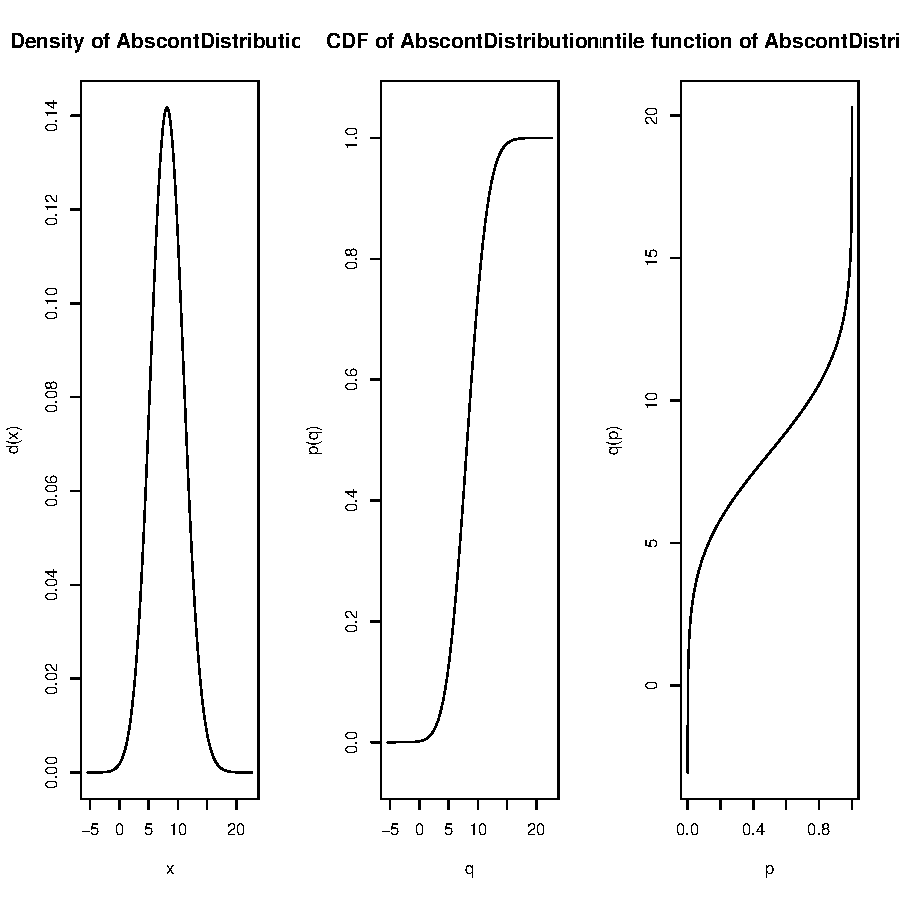
\includegraphics{distr-exam1}
\par
\begin{small}
\noindent{\bf Comment:}\\
Let \code{N} an object of class \code{"Norm"} with parameters  \code{mean=2},
\code{sd=1.3} and let \code{P}  an object of class \code{"Pois"} with parameter 
\code{lambda=1.2}. Assigning to \code{Z} the expression \code{2*N+3+P}, a 
new distribution object is generated ---of class \code{"AbscontDistribution"} in our case--- so that identifying \code{N}, \code{P}, \code{Z} with random variables
distributed according to {\tt N}, {\tt P}, {\tt Z}, 
${\cal L}({\tt Z})={\cal L}(2*{\tt N}+3+{\tt P})$,  and writing \code{p(Z)(0.4)}  we get $P(Z\leq 0.4)$, \code{ q(Z)(0.3)}  the $30\%$-quantile of {\tt Z},
and with \code{r(Z)(50)} we generate $50$ pseudo random numbers distributed according to {\tt Z}, while the \code{plot} command generates the above figure.
\end{small}
% -------------------------------------------------------------------------------
\section{Concept}
% -------------------------------------------------------------------------------
In developing our packages, we had the following principles in mind:
We wanted to be open in our design so that our classes could easily be extended by 
any volunteer in the {\sf R} community to provide more complex classes of 
distributions as multivariate distributions, times series distributions, conditional
distributions. As an exercise, the reader is encouraged to implement extrem value  distributions from the package \pkg{evd}\footnote{a solution to this ``homework'' 
may be found in the sources to \pkg{distrEx}}. The largest effort will in fact be the 
documentation\ldots\\
We also wanted to preserve naming and notation from {\sf R}-\pkg{stats}
as far as possible so that any programmer used to {\tt S} could quickly
use our package. Even more so, as the distributions already implemented to
{\sf R} are all well tested and programmed with skills we lack, we use the
existing {\tt r}, {\tt d}, {\tt p}, and {\tt q}-functions wherever possible,
only wrapping them by small code sniplets to our class hierarchy.\\
Third we wanted to use a suggestive notation for our automatically generated
methods \code{r}, \code{d}, \code{p}, and \code{q}, which we think is now largely achieved.
All this should make intensive use of object orientation in order to be able to use 
inheritance and method overloading.
Let us briefly explain why we decided to realize \code{r}, \code{d},
\code{p}, and \code{q} as part of our class definitions:
Doing so, we place ourselves somewhere between
pure object orientation where methods would be {\it slots\/} ---in the language of the {\tt S4}-concept,
confer \cite{Cham:98}--- and the {\tt S4} paradigm where methods "live their own life"
apart from the classes, or, to \code{q}, which should be regarded use 
\cite{Beng:03}'s terminology, we use COOP\footnote{class-object-orientated 
programming, as e.g.\ in {\tt C++}}-style for \code{r}, \code{d}, \code{p}, and 
\code{q} methods, and FOOP\footnote{function-object-orientated programming, 
as in the {\tt S4}-concept} -style for "normal" methods.\\
The {\tt S4}-paradigm with methods which are not attached to an object but rather 
behave differently according to the classes of their arguments is fine if there are
particular user-written methods for only some few general distribution classes like 
\code{AbscontDistribution}, as in the case for \code{plot} or \code{"+"} 
(c.f.\ \cite{K:R:S:04}, Section 2.2). 
During a typical {\sf R} session with \pkg{distr}, however, there will be a lot of, 
mostly automatically generated objects of our distribution classes, each with its 
own \code{r}, \code{d}, \code{p}, and \code{q}; this even applies to 
intermediate expressions like \code{2*N}, \code{2*N+3} to eventually produce 
\code{Z} in the example in the motivation. Treating \code{r}, \code{d}, 
\code{p}, and \code{q} as generic functions, we would need to generate new 
classes for each expression \code{2*N}, \code{2*N+3}, \code{Z} and, 
correspondingly, particular {\tt S4}-methods for \code{r}, \code{d}, \code{p}, 
and \code{q} for each of these new classes; apparently, this would produce overly 
many classes for an effective inheritance structure. \\
In providing arithmetics for distributions, we have to deviate a little from
the paradigm of {\tt S} as a functional language: For operators like ``$+$'',
additional parameters controlling the precision of the results cannot be handily
passed as arguments. For this purpose we provide global options which may be
inspected and modified by \code{distroptions}, \code{getdistrOption}\footnote{Upto version 0.4-4,
we use a different mechanism to inspect/modify global options of \pkg{distrEx}
(see section~\ref{distrExoptions}); corresponding functions \code{distrExoptions}, \code{getdistrExOption}
for package \pkg{distrEx} will only be available from version 0.4-5 on, which is
due for spring 2007.} in complete analogy to \code{options}, \code{getOption}.
%
Finally our concept as to parameters: Contrary to the standard {\sf R}-functions like 
\code{rnorm} we only permit length $1$ for parameters like \code{mean}, because 
we see the objects as implementations of univariate random variables, for which 
vector-valued parameters make no sense; rather one could gather several objects 
with possibly different parameters to a vector/list of distributions. Of course, the 
original functions \code{rnorm} etc.\ remain unchanged and still allow for 
vector-valued parameters.
Kouros Owzar  in an off-list mail raised the point, that in case of multiple parameters 
as in case of the normal or the $\Gamma$-distribution, it might be useful to be able 
to pass these multiple parameters in vectorized form to the generating function. 
We, too, think that this is a good idea, but even more plan to introduce a further
extension package to \pkg{distr} which will cover statistical models. In this package, 
this issue will be solved by requiring a map $\theta \mapsto P_\theta$ or, in {\tt S}, 
a function \code{function(theta){....}} which returns an object of class distribution 
or subclass, which realizes $P_\theta$. So it will be up to the programmer or user how 
to realize this map.
% -------------------------------------------------------------------------------
\section{Organization in classes}
% -------------------------------------------------------------------------------
Loosely speaking we have three large groups of classes: distribution classes (in 
\pkg{distr}), simulation classes (in \pkg{distrSim}) and an evaluation class (in 
\pkg{distrTEst}), where the latter two are to be considered only as tools which 
allow a unified treatment of simulations and evaluation of statistical estimation 
(perhaps also tests and predictions later) under varying simulation situations.
Additionally, package \pkg{distrEx} provides classes for discrete multivariate 
distributions and for factorized, conditional distributions, as well as a bundle of 
functionals and distances (see below).
% -------------------------------------------------------------------------------
\subsection{Distribution classes}
% -------------------------------------------------------------------------------
The purpose of the classes derived from the class \code{Distribution}  is to implement 
the concept of a r.v./distribution as such in {\sf R}.\\
All classes derived from \code{Distribution} have a slot \code{param} for a 
parameter, a slot \code{img} for the range and the constitutive slots \code{r}, 
\code{d}, \code{p}, and \code{q}.
% -------------------------------------------------------------------------------
\subsubsection{Subclasses}
% -------------------------------------------------------------------------------
To begin with, we limit ourselves to univariate distributions giving the {\tt S4}-class 
\code{UnivariateDistribution}, and as typical subclasses, we introduce classes for 
absolutely continuous and discrete distributions ---\code{AbscontDistribution} and
\code{DiscreteDistribution}.
The latter has a slot \code{support}, a vector containing the support of the 
distribution, which is truncated to the lower/upper \code{TruncQuantile} in case of 
an infinite support. \code{TruncQuantile} is a global option of  \pkg{distr} described
in section~{\ref{options}}.\\
As subclasses of these two classes, we have implemented all parametric families 
which already exist in the  \pkg{stats} package of {\sf R} in form of 
{\tt [prefix]<name>} functions ---by just providing wrappers to the original 
{\sf R}-functions. Schematically, the inheritance relations as well as the slots of 
the corresponding classes may be read off from figure~\ref{fig1c}.
\ifpdf
\begin{figure}[!ht]\label{fig1}
\vspace{2ex}
  \begin{center}
%    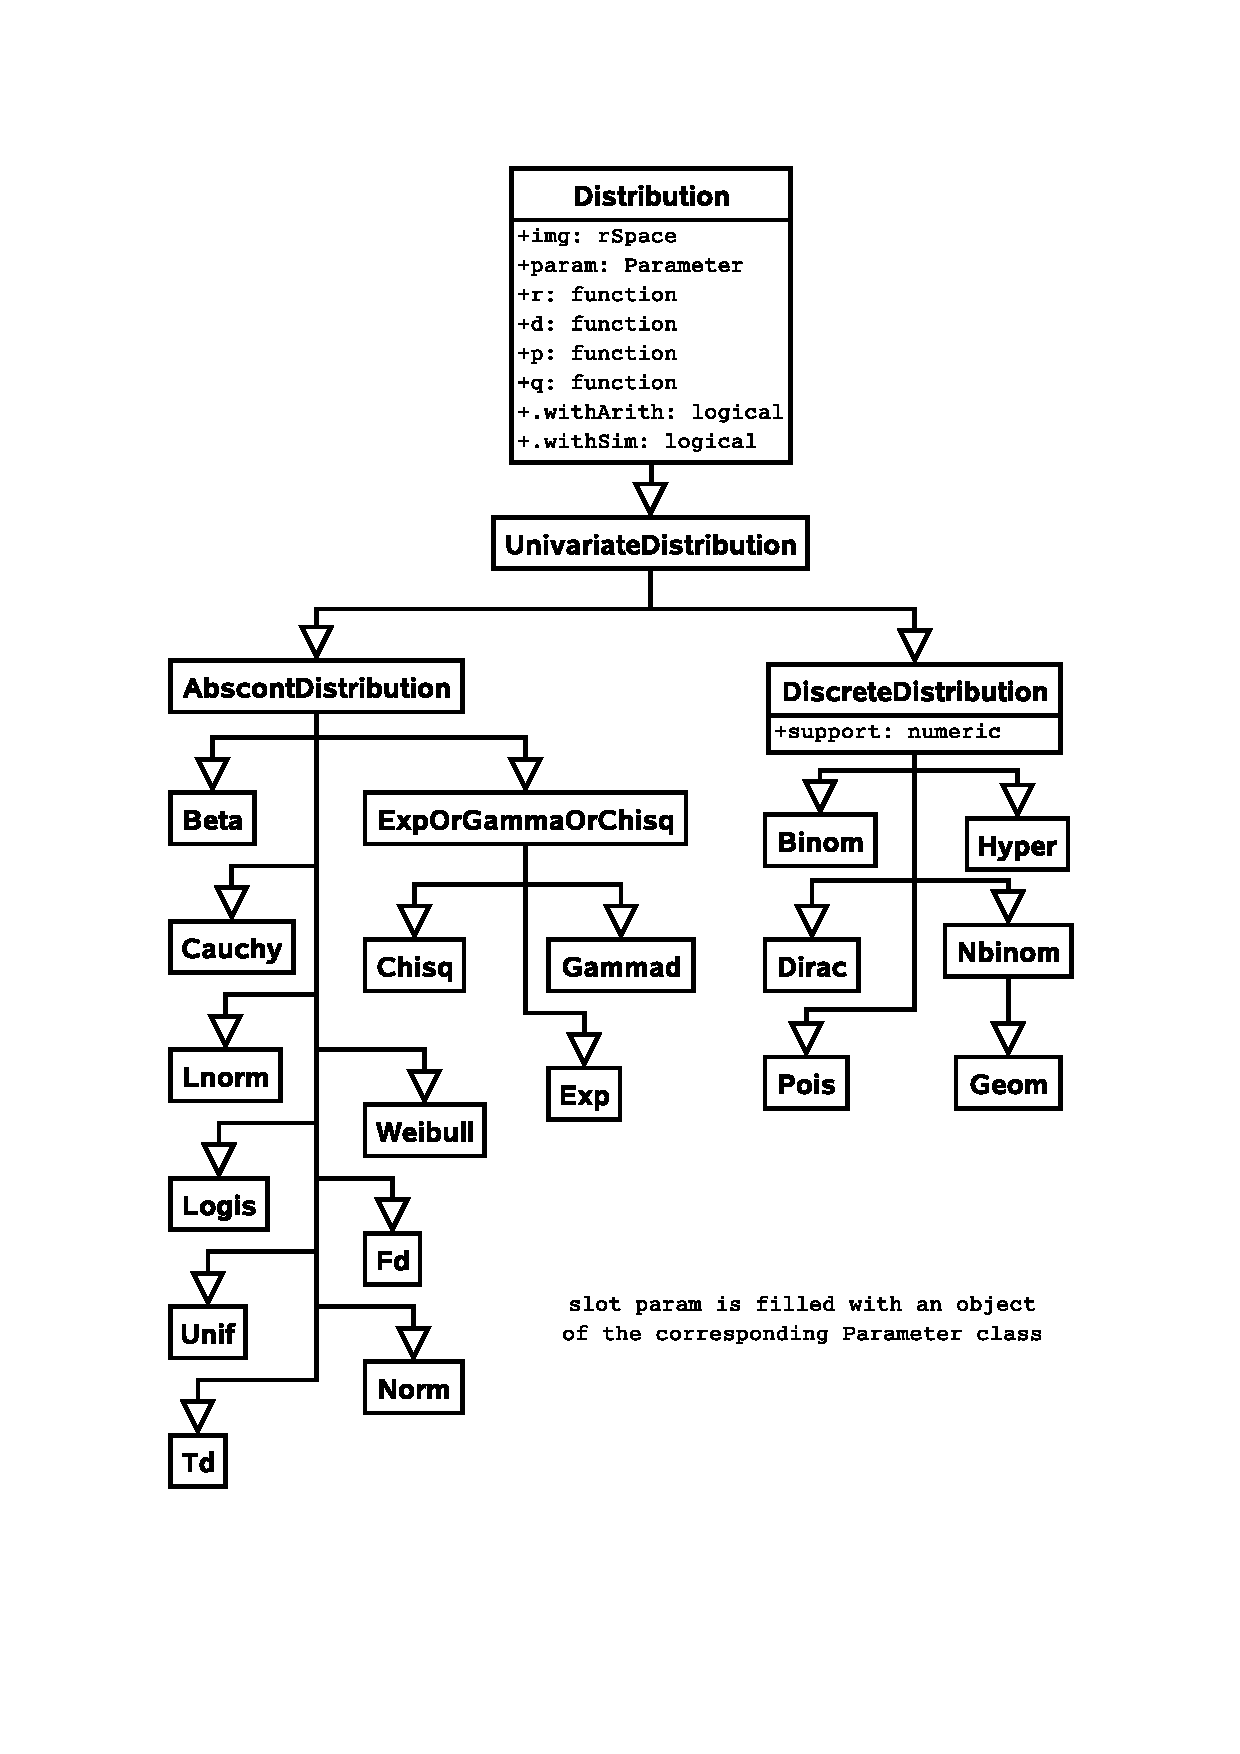
\includegraphics[viewport=0 0 500 700,width=9cm]{distribution.pdf}%
    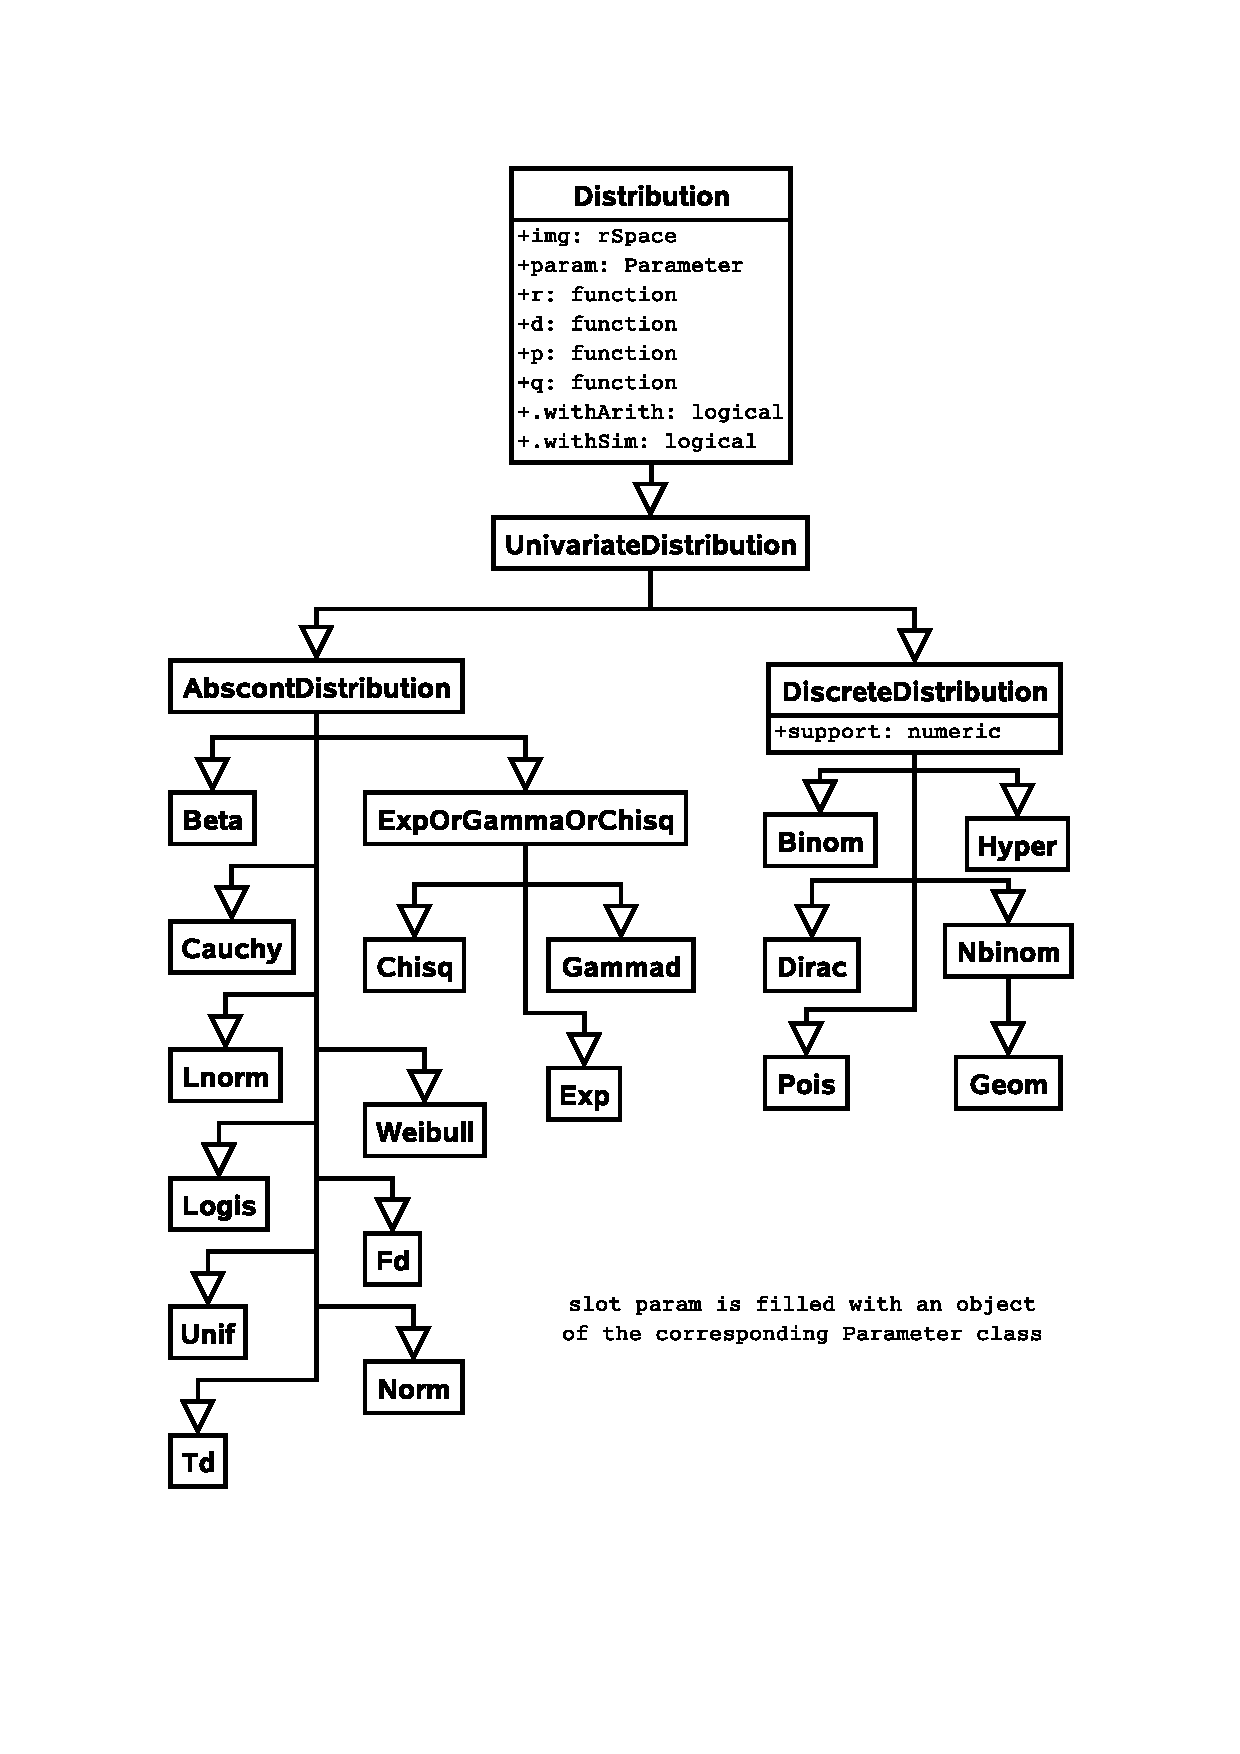
\includegraphics[viewport=130 150 500 750,width=9cm]{distribution.pdf}%
    \caption{\label{fig1c}{\footnotesize Inheritance relations and slots of the corresponding \mbox{(sub-)}classes
    for \code{Distribution} where we do not repeat inherited slots
    }}
  \end{center}
\vspace{-4ex}
\end{figure}
\else
\begin{figure}[htb]\label{fig1}
  \begin{center}
    \includegraphics[viewport=130 150 500 730,width=7.5cm]{distribution.ps}%
    \caption{\label{fig1c}{\footnotesize Inheritance relations and slots of the corresponding \mbox{(sub-)}classes
    for \code{Distribution} where we do not repeat inherited slots
    }}
  \end{center}
\vspace{-1ex}
\end{figure}
\fi
Operations to automatically generate new slots \code{r}, \code{d}, \code{p}, and \code{q} ---induced by
mathematical transformations--- perhaps provide the most powerful use of our package. This is discussed in
some detail in subsection~{\ref{methods}}.
%
\subsubsection{Classes for multivariate distributions and for conditional distributions}

In \pkg{distrEx}, we provide the following classes for handling multivariate distributions:

\paragraph{Lists of distributions}

As a first step, we allow distributions to be gathered in lists, giving
classes \code{DistrList} and \code{UnivarDistrList}, where in case of the latter,
all elements must be univariate distributions. For these, the usual indexing operations
with \code{[[.]]} are available.

\paragraph{Multivariate distribution classes}

Multivariate distributions are much more complicated than univariate ones,
which is why but a few exceptional ones have already been implemented to R in
packages like \pkg{multnorm}. In particular it is not so clear what a slot \code{q}
should mean and, in higher dimensions slot \code{p}, and possibly also slot \code{d}
may become awkward. So, for multivariate distributions, realized as class
\code{MultivariateDistribution}, we only insist on slot \code{r}, while the other
functional slots may be left void.

The easiest case is the case of a discrete multivariate distribution with finite support
which is implemented as class \code{DiscreteMVDistribution}.

\paragraph{Conditional distribution classes}

Also arising in multivariate settings only are conditional distributions. In our approach,
we realize factorized, conditional distributions where the (factorized) condition is in
fact treated as an additional parameter to the distribution. The condition is realized
as an object of class \code{Condition}, which is a slot of corresponding classes
\code{UnivariateCondDistribution}. This latter is the mother class to classes
\code{AbscontCondDistribution} and \code{DiscreteCondDistribution}.
The most important application of these classes so far is regression, where
the distribution of the observation given the covariates is just realized as
a \code{UnivariateCondDistribution}.

\subsubsection{Parameter classes}
%
As most distributions come with a parameter which often is of own interest, we endow
the corresponding slots of a distribution class with an own parameter class, which
allows for some checking like ``Is the parameter \code{lambda} of an exponential distribution non-negative?'',
``Is the parameter \code{size} of a binomial a positive integer?''\\
Consequently, we have a method \code{liesIn} that may answer such questions by a \code{TRUE}/\code{FALSE}
statement. Schematically, the inheritance relations of class \code{Parameter} as well as the slots of the corresponding
\mbox{(sub-)}classes may be read off in figure~\ref{fig4c} where we do not repeat inherited slots.
%
\ifpdf
\begin{figure}[!ht]\label{fig4}
  \begin{center}
%    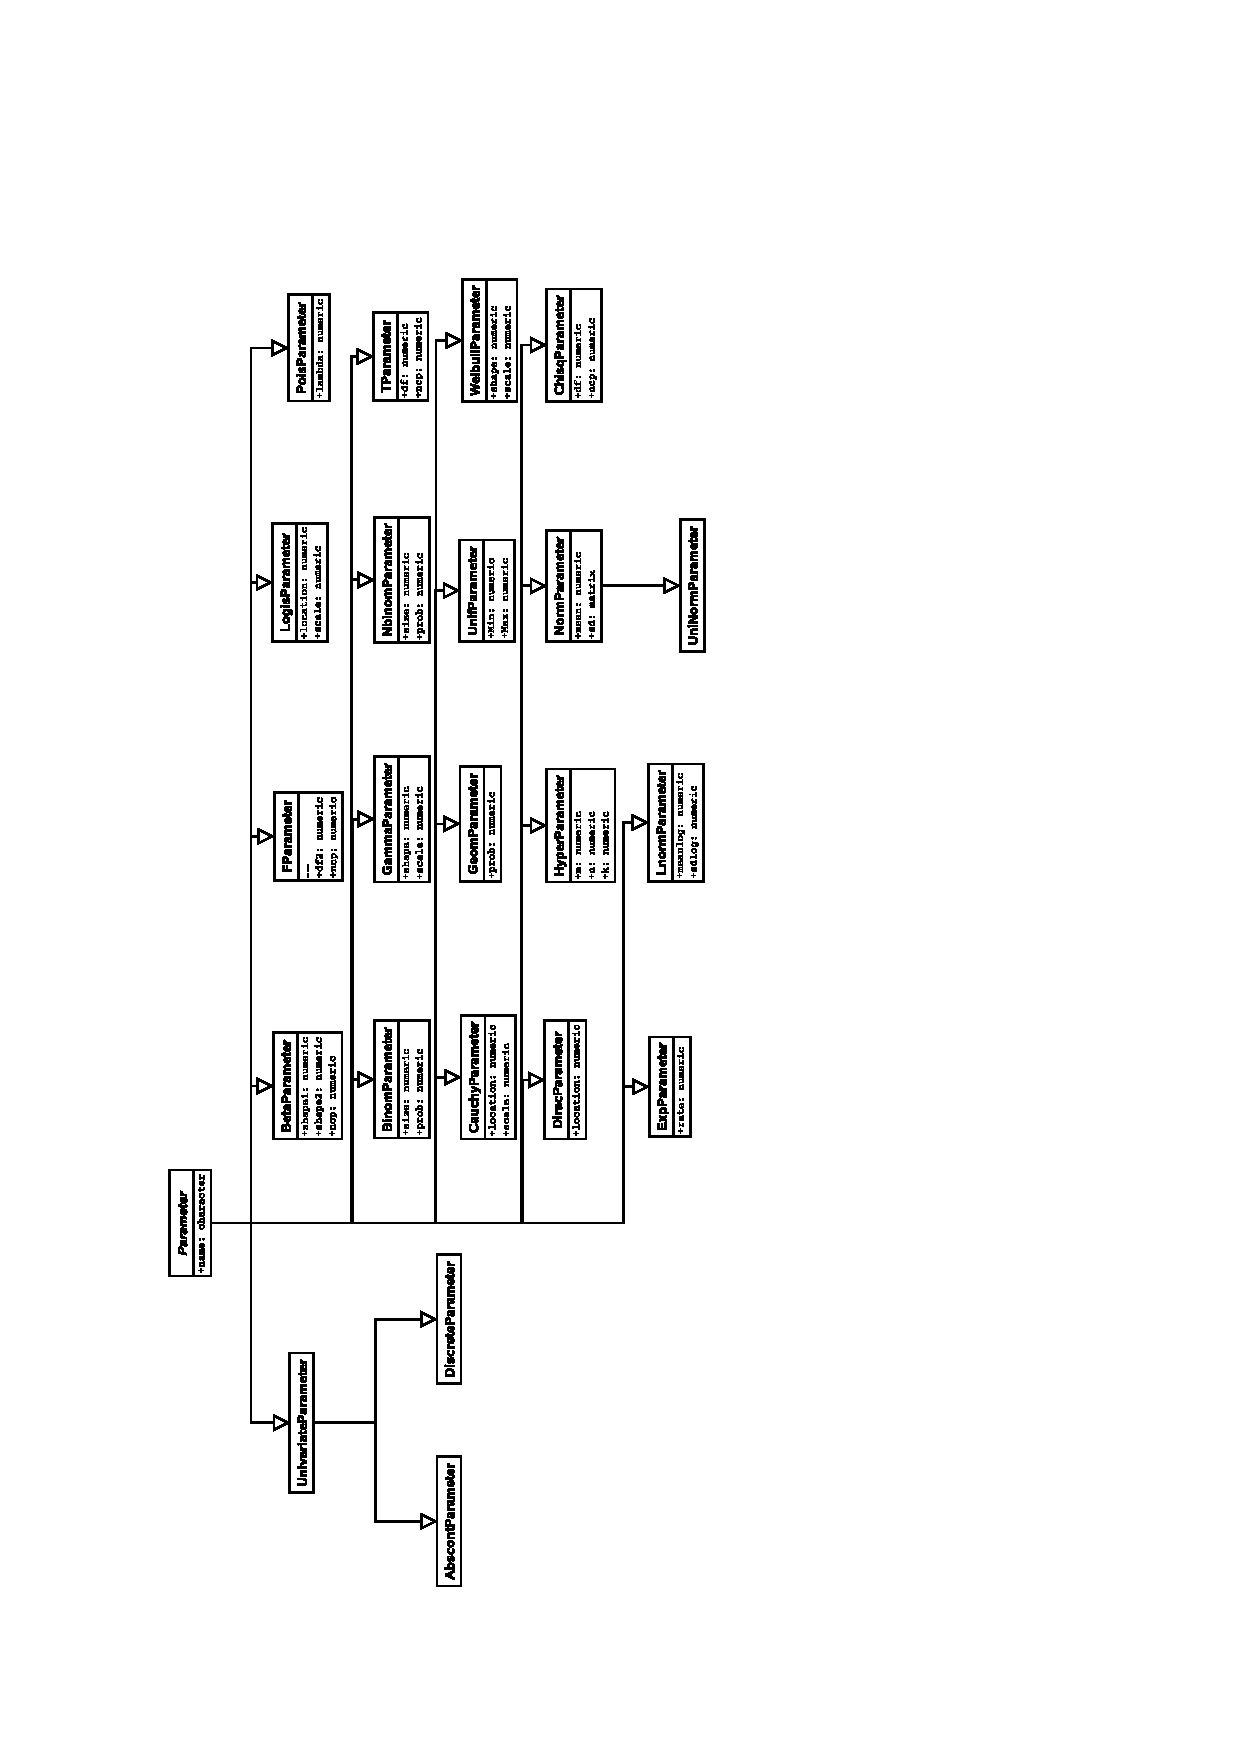
\includegraphics[viewport=30 10 540 390,height=11cm,width=12cm]{parameter.pdf}%[viewport=30 10 540 390,width=12.cm]
    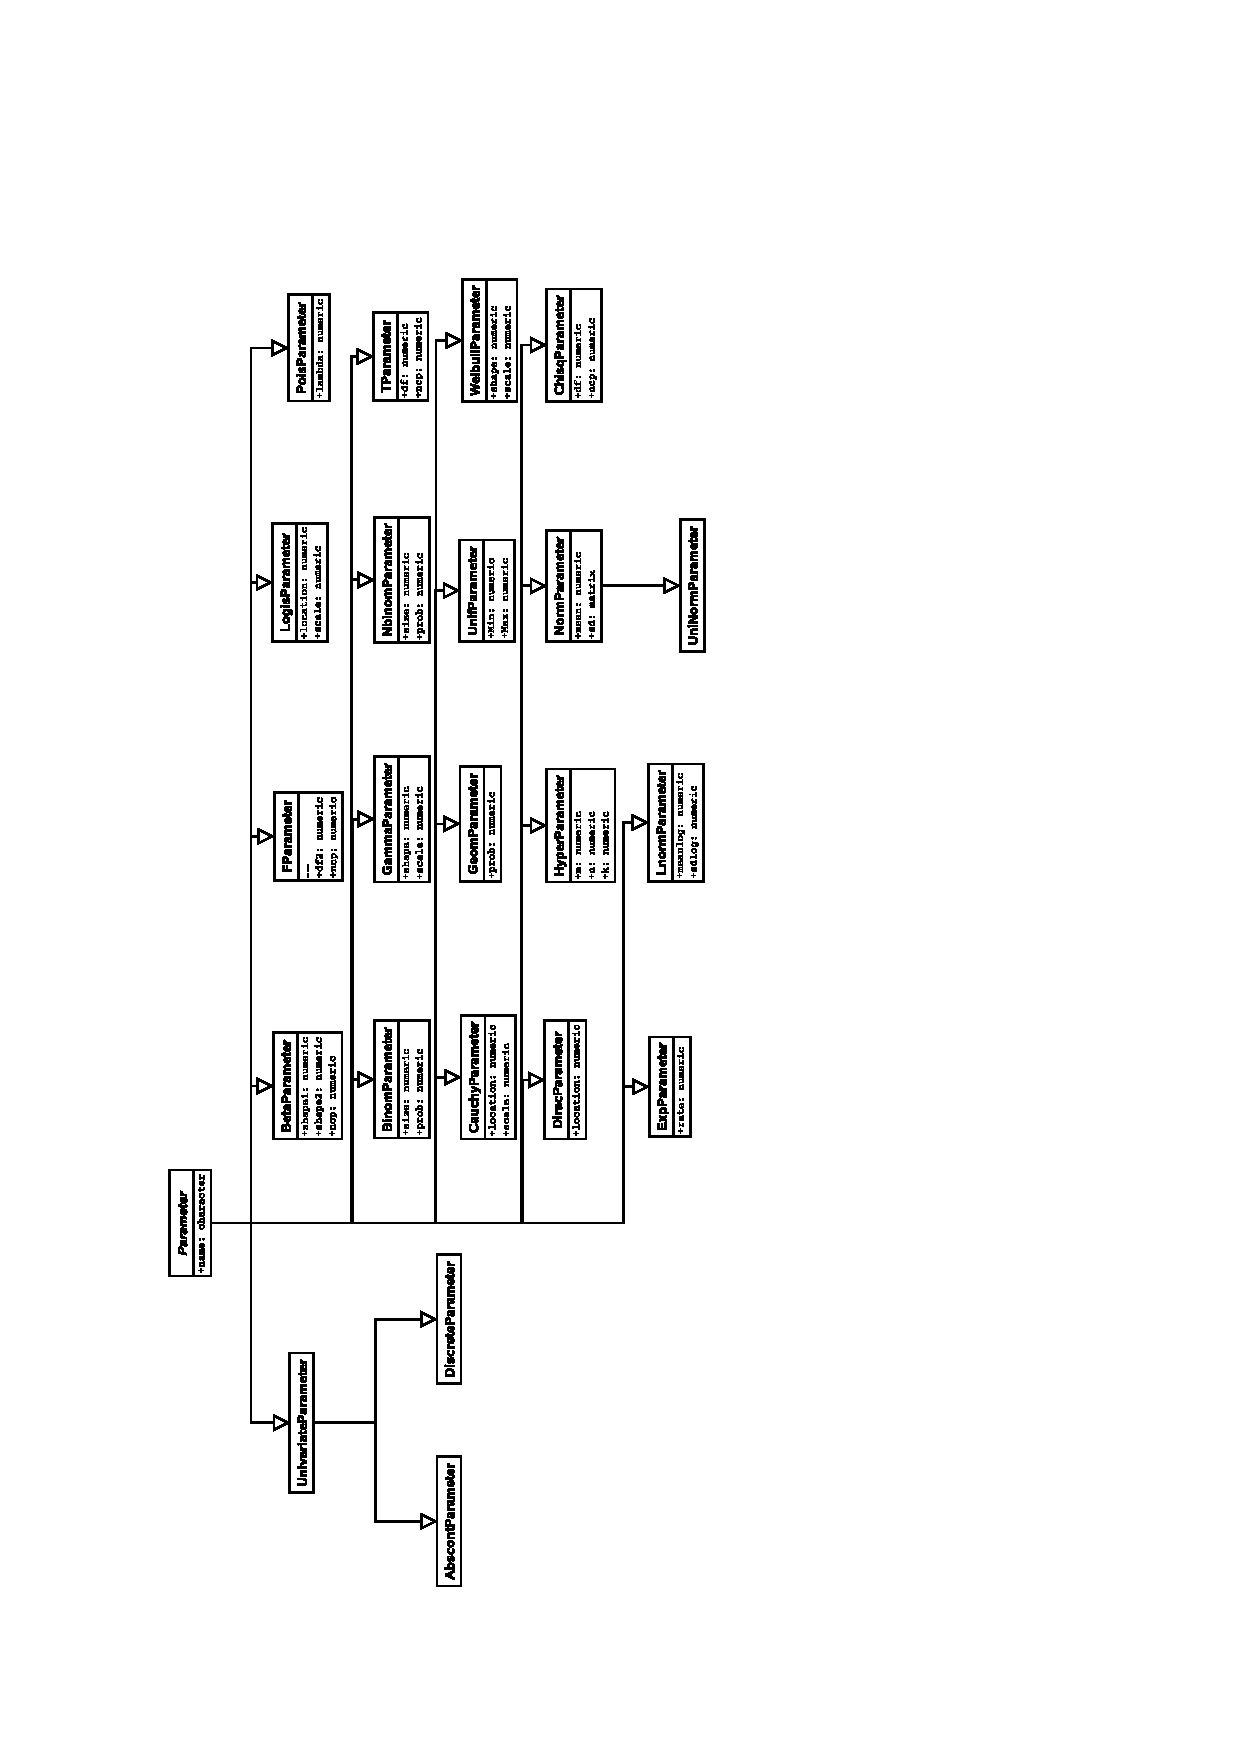
\includegraphics[viewport=30 80 400 690,height=15cm,width=12cm]{parameter.pdf}%[viewport=30 10 540 390,width=12.cm]
    \caption{\label{fig4c}{\footnotesize Inheritance relations and slots of the corresponding \mbox{(sub-)}classes
    for \code{Parameter}
    }}
  \end{center}
\end{figure}
\else
\begin{figure}[htb]\label{fig4}
  \begin{center}
    \includegraphics[viewport=80 120 340 600,height=12.8cm,width=9.0cm, angle=-90]{parameter.ps}%
    \caption{\label{fig4c}{\footnotesize Inheritance relations and slots of the corresponding \mbox{(sub-)}classes
    for \code{Parameter}
    }}
  \end{center}
\end{figure}
\fi
%
The most important set to be used as parameter domain/sample space (\code{rSpace}) will be
an Euclidean space. So \code{rSpace} and \code{EuclideanSpace} are also implemented as classes,
 the structure of which may be read off in figure~\ref{fig5c}.
\begin{figure}[htb]\label{fig5}
  \begin{center}
    \ifpdf
    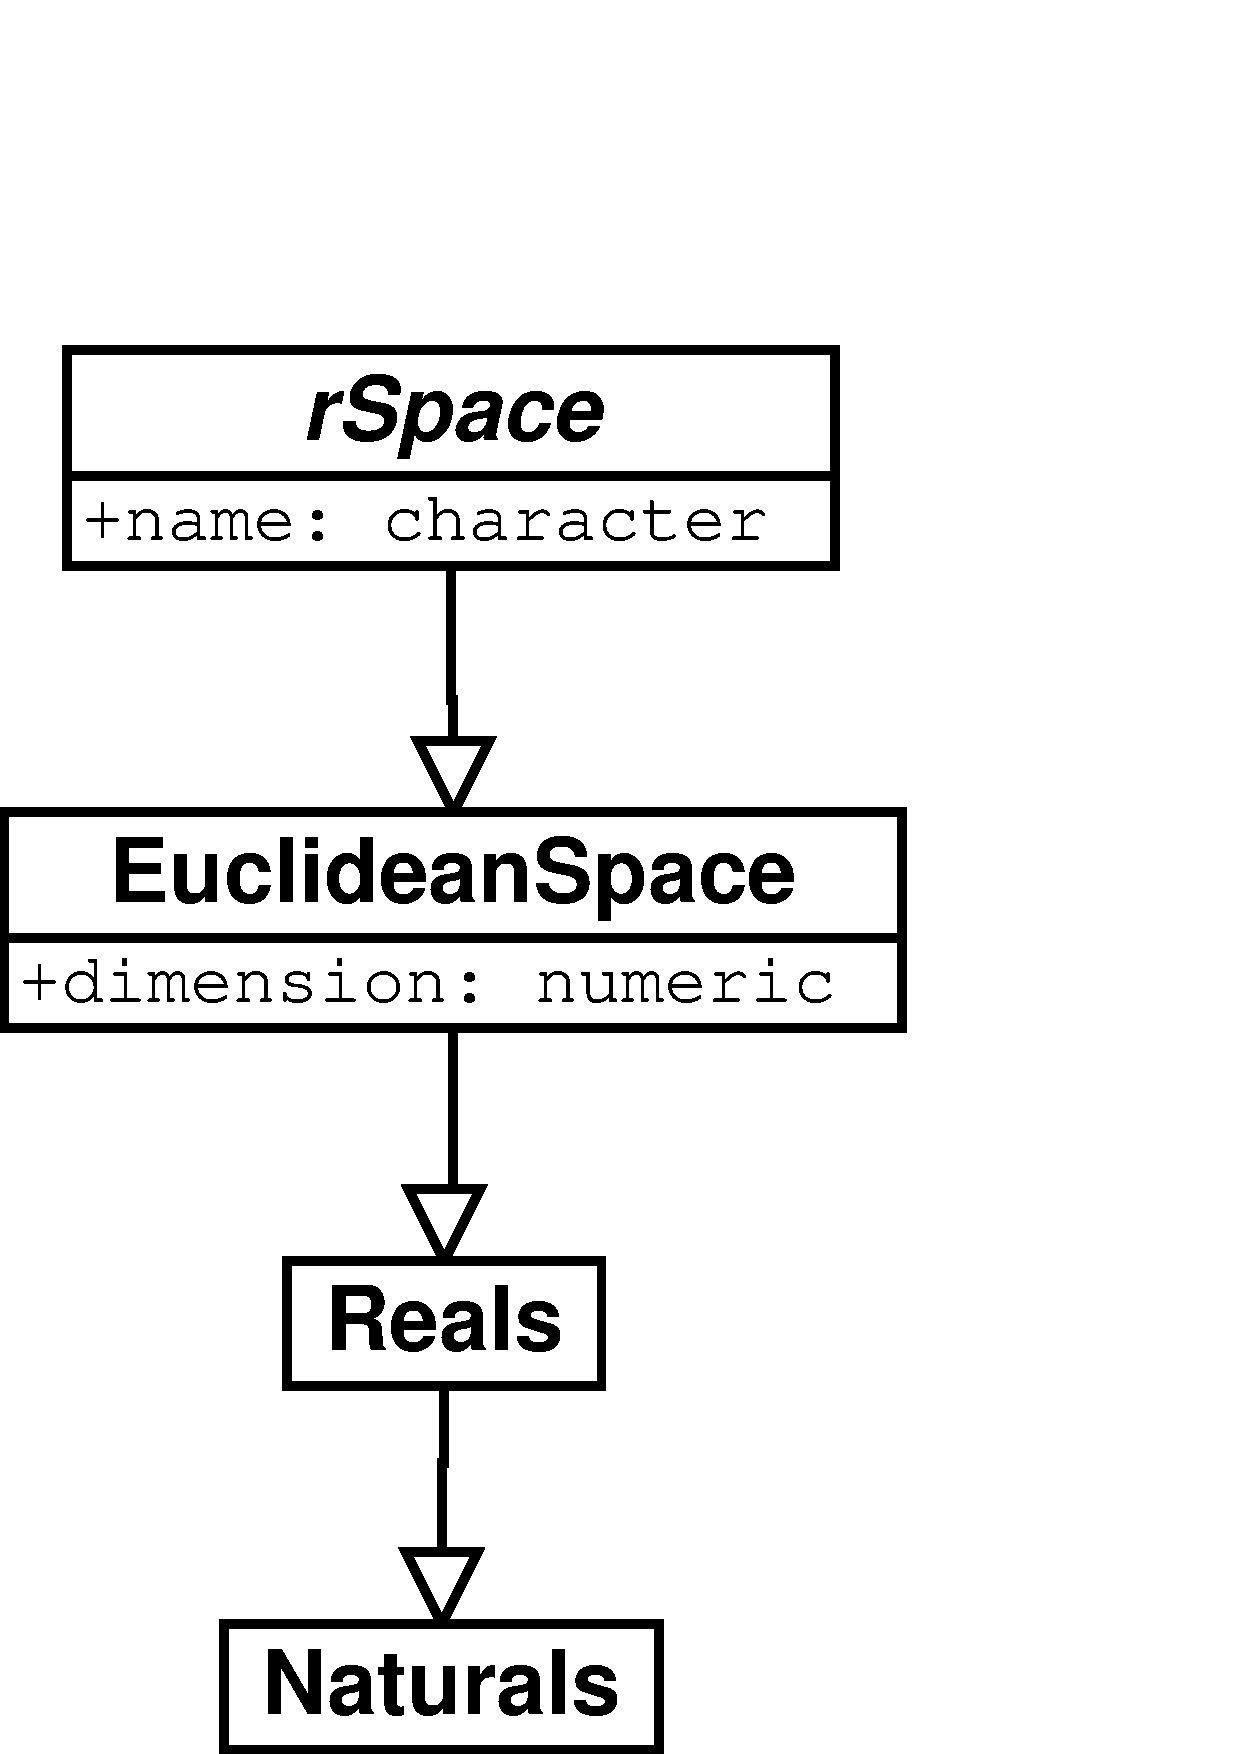
\includegraphics[%viewport=0 30 600 600,
    width=3.9cm]{rspace.pdf}
    \else
    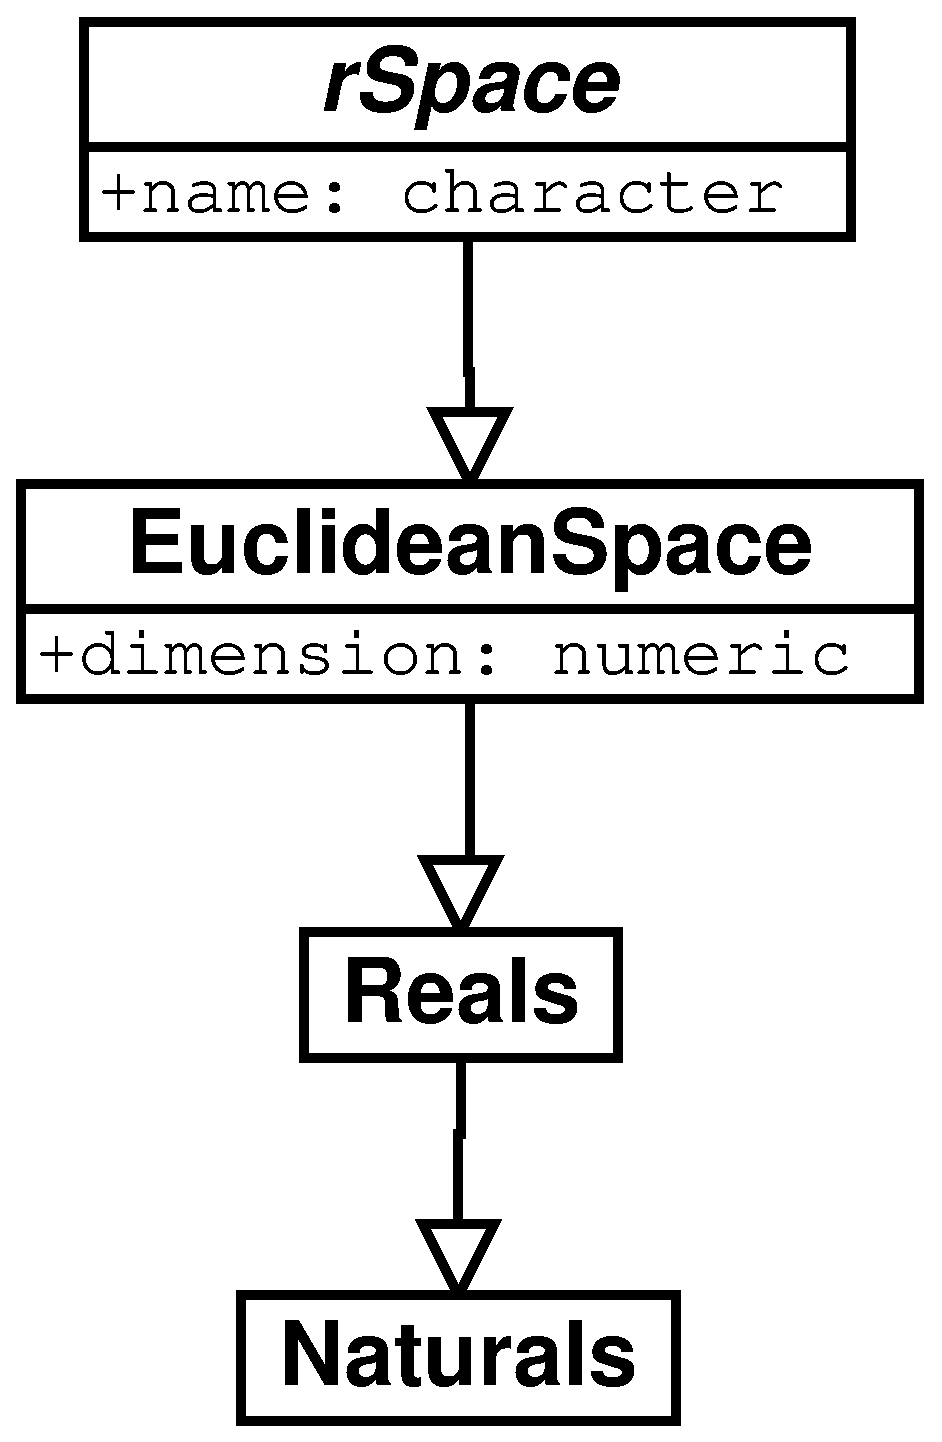
\includegraphics[width=3.7cm]{rspace.ps}%
    \fi
    \caption{\label{fig5c}{\footnotesize Inheritance relations and slots of the corresponding \mbox{(sub-)}classes
    for \code{rSpace}
    }}
  \end{center}
\end{figure}

\subsection{Simulation classes}
From version 1.6 on, the classes and methods of this subsection are available in package  \pkg{distrSim}.

The aim of simulation classes is to gather all relevant information about a simulation
in a correspondingly designed class. To this end we introduce the class \code{Dataclass}
that serves as a common mother class for both "real" and simulated data.
%
As derived classes we then have a simulation class where we also gather all information
needed to reconstruct any particular simulation.\\
%
%\newline0??????\\
From version 1.8 of this package on, we have changed the
format how data / simulations are stored:
In order to be able to cope with multivariate,
regression  and (later) time series distributions,
we have switched to the common array format
%
{\tt samplesize x obsDim x runs} where {\tt obsDim} is the dimension of the observations.
%
For saved objects from earlier versions, we provide the functions
\code{isOldVersion} and \code{conv2NewVersion} to check whether the
object was generated by an older version of this package and
to convert such an object to the new format, respectively.
For objects generated from version 1.8 on, you get the package 
version of package~\pkg{distrSim}, under which they have been generated
by a call to \code{getVersion()}. \\
%
%??????1\\
 Finally, coming from robust statistics
we also consider situations where the majority of the data stems from an ideal situation/distribution
whereas a minority comes from a contaminating source. To be able to identify ideal and
contaminating observations, we also store this information in an indicator variable.\\
%
As the actual values of the simulations only play a secondary role, and as the number of
simulated variables can become very large, but still easily reproducible, it is not worth
storing all simulated observations but rather only the information needed to reproduce the simulation.
This can be done by \code{savedata}.\\
Schematically, the inheritance relations of class \code{Dataclass} as well as the slots of the corresponding
\mbox{(sub-)}classes may be read off in figure~\ref{fig2c} where we do not repeat inherited slots.
\begin{figure}[htb]\label{fig2}
  \begin{center}
    \ifpdf
    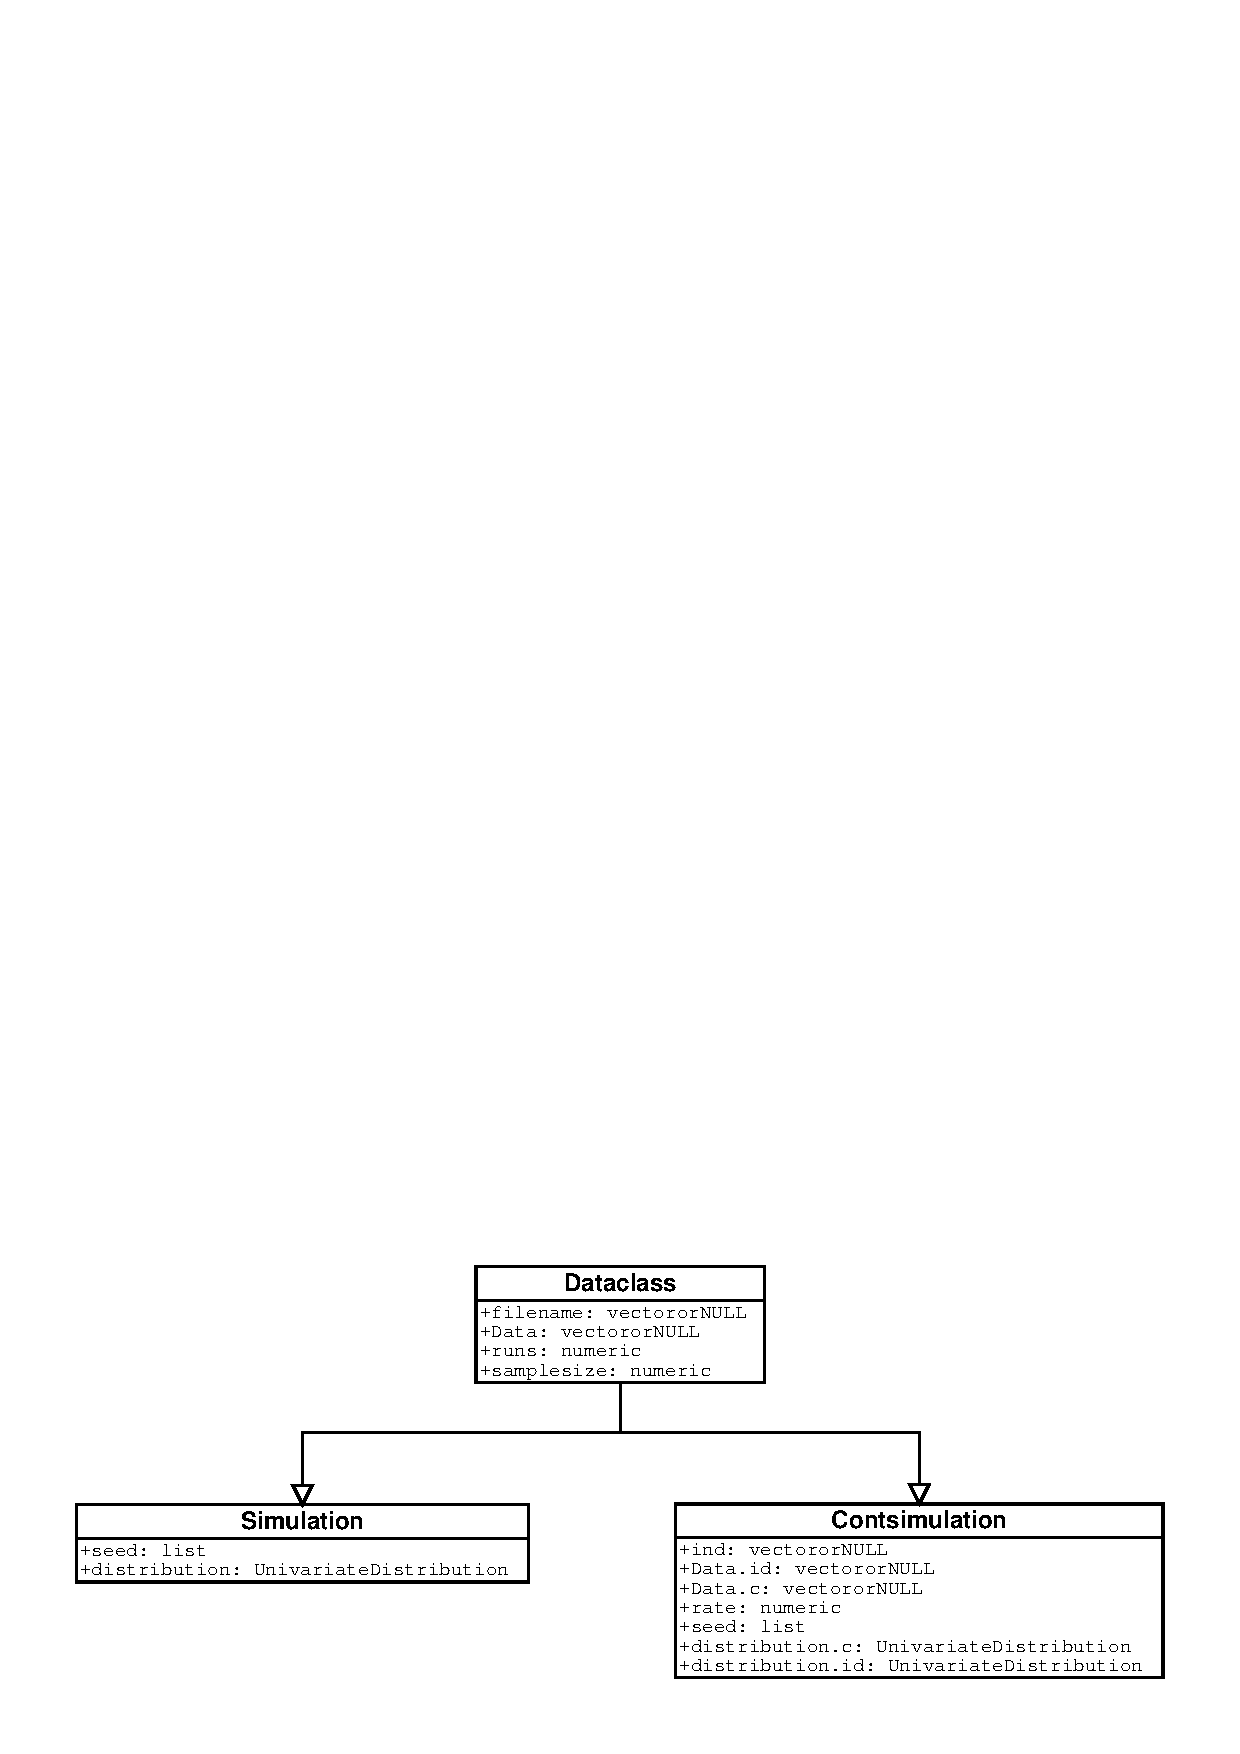
\includegraphics[viewport=120 30 470 250,width=8.5cm]{dataclass.pdf}
    \else
    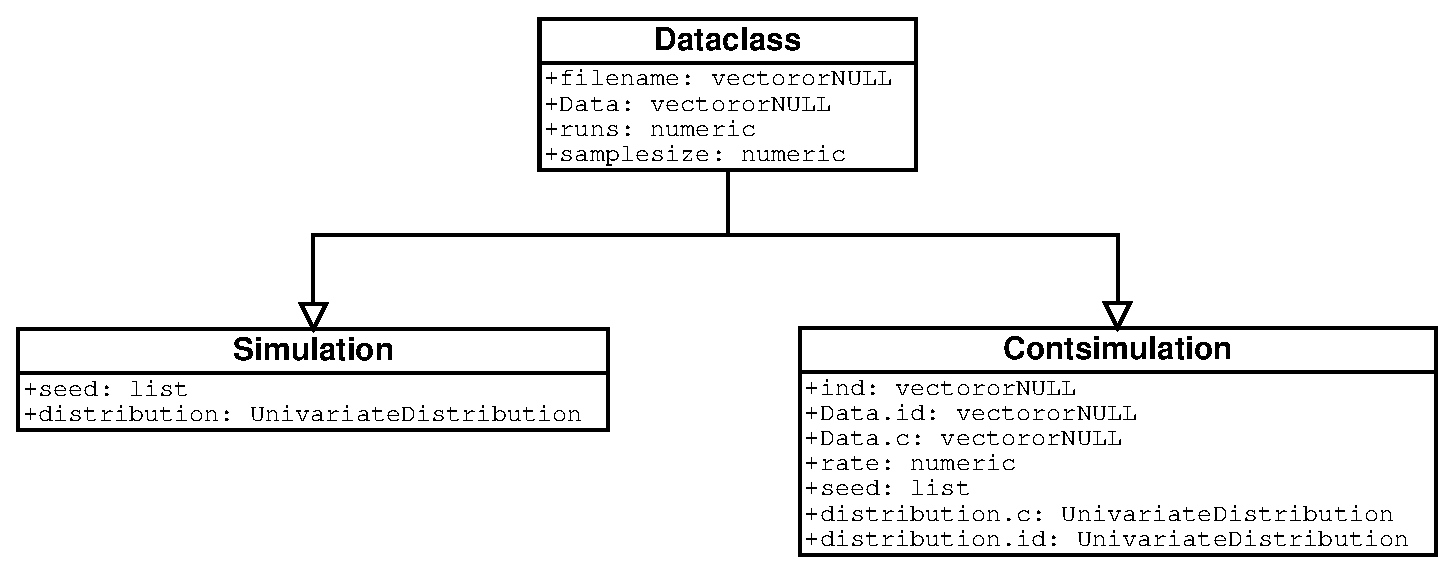
\includegraphics[width=12.5cm]{dataclass.ps}%
    \fi
    \caption{\label{fig2c}{\footnotesize Inheritance relations and slots of the corresponding \mbox{(sub-)}classes
    for \code{Dataclass}
    }}
  \end{center}
\end{figure}
%\newline0??????\\
Also, analogously to  package%s
 \pkg{distr}, %and \pkg{distrEx},
 global options for the output by methods \code{plot} and \code{summary}
are controlled by \code{distrSimoptions()} and \code{getdistrSimoptions()}\smallskip\\
%??????1\\

\subsection{Evaluation class}
From version 1.6 on, the class and methods of
this subsection are available in package  \pkg{distrTEst}. \\
When investigating properties of a new procedure (e.g. an estimator) by means of simulations,
one typically evaluates this procedure on a large set of simulation runs and gets a result for
each run. These results are typically not available within seconds, so that it is worth storing them.
To organize all relevant information about these results, we introduce a class \code{Evaluation} the slots of
which is filled by method \code{evaluate} ---see subsection~\ref{evaluate}.
Schematically, the slots of this class may be read off in figure~\ref{fig3c}.
\begin{figure}[htb]\label{fig3}
  \begin{center}
    \ifpdf
    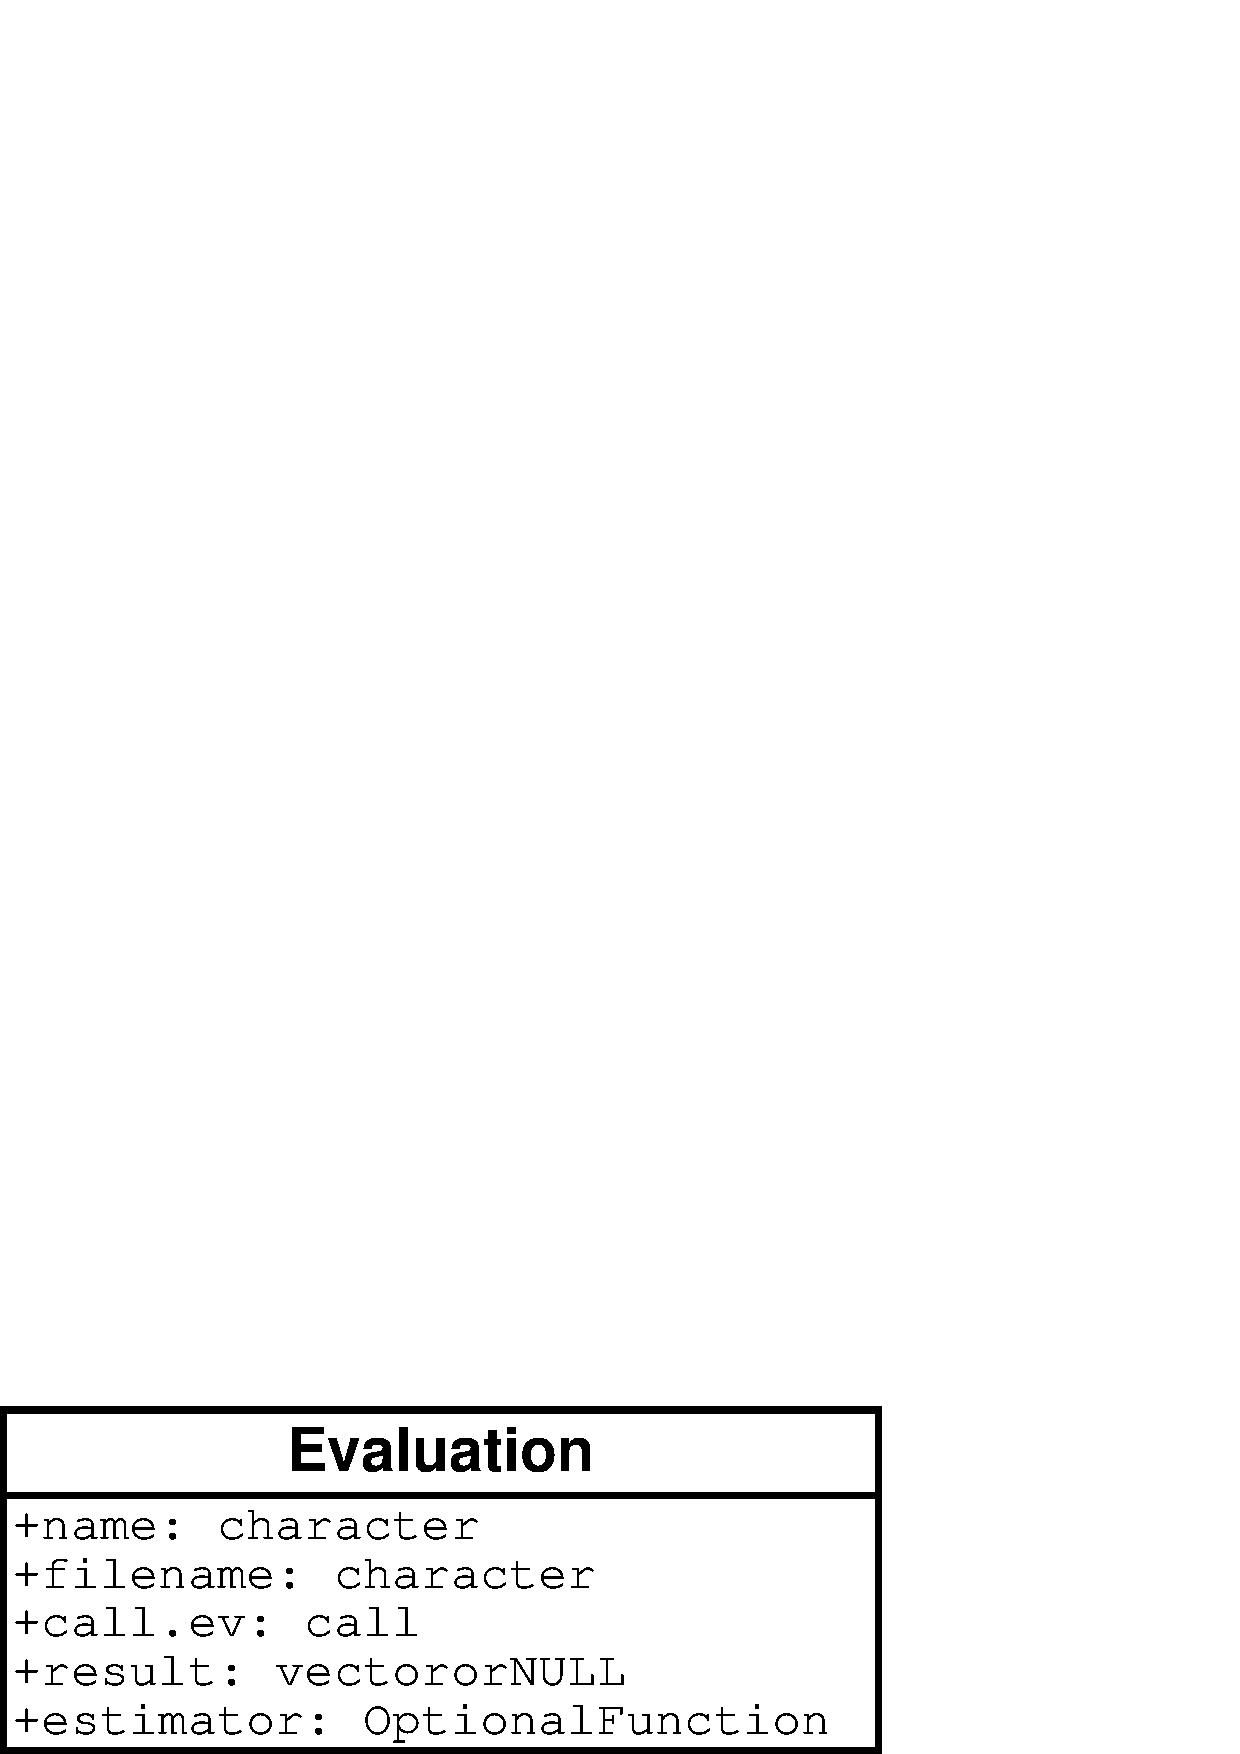
\includegraphics[viewport=60 20 420 200,width=5cm]{evaluation.pdf}
    \else
    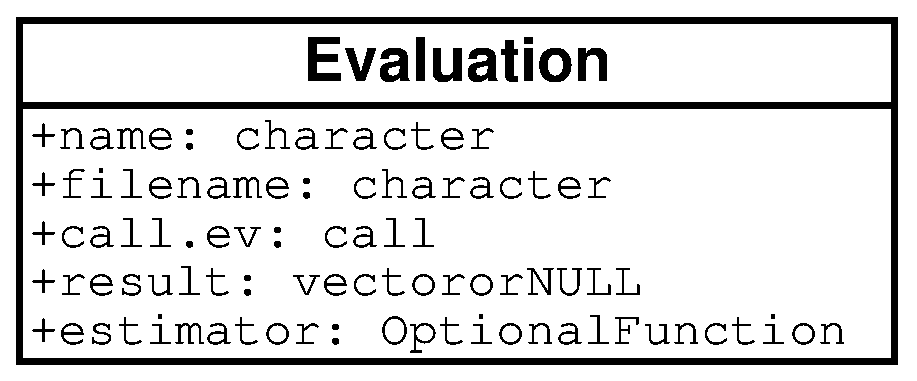
\includegraphics[width=5cm]{evaluation.ps}%
    \fi
    \caption{\label{fig3c}{\footnotesize Slots of class \code{Evaluation}}}
  \end{center}
\end{figure}
%\newline0??????\\
A corresponding \code{savedata} method
saves the object of class \code{Evaluation} in two files in the {\sf R}-working directory: one
using the filename \code{<filename>} also stores the results; the other one,
designed to be ``human readable'', comes as a comment file with filename \code{<filename>.comment}
only stores the remaining information.
The filename can be specified in the optional argument \code{fileN} to \code{savedata}; by default it is concatenated
from the \code{filename} slot of the \code{Dataclass} object and \code{<estimatorname>}, which you may either
pass as argument \code{estimatorName} or by default is taken as the {\sf R}-name of the corresponding {\sf R}-function
specified in slot \code{estimator}.

From version 1.8 on, slot \code{result} in class \code{Evaluation} is of class \code{DataframeorNULL},
i.e.; may be either a data frame or {\tt NULL}, and slot \code{call.ev} in class \code{Evaluation}
is of class "CallorNULL", i.e.; may be either a call or {\tt NULL}.
Also, we want to gather \code{Evaluation} objects in a particular data structure \code{EvaluationList}
(see below), so we have to be able to check whether all data sets in the gathered objects coincide.
For this purpose, from this version on, class \code{Evaluation} has an additional slot \code{Data} of
class \code{Dataclass}. In order not to burden the objects of this class too heavily with uninformative
simulated data, in case of a slot \code{Data} of one of the simulation-type subclasses of \code{Dataclass},
this \code{Data}  itself has an empty \code{Data}-slot.\\

\subsection{EvaluationList class}
The class and methods of this subsection are available in package  \pkg{distrTEst}. \\
In order to compare different procedures / estimators for the
same problem, it is natural to gather several \code{Evaluation} objects
with results of the same range (e.g.\ a parameter space) generated on the
same data, i.e.; on the same \code{Dataclass} object. To this end, from
version 1.8 on, we have introduced class \code{EvaluationList}.
Schematically, the slots of this class may be read off in figure~\ref{fig3c1}.
\begin{figure}[htb]\label{fig3-1}
  \begin{center}
%    \ifpdf
%    \includegraphics[viewport=60 20 420 200,width=5cm]{evaluationlist.pdf}
%    \else
%    \includegraphics[width=5cm]{evaluationlist.ps}%
%    \fi
\parbox{10cm}{HIER KOMMT DAS BILD}
    \caption{\label{fig3c1}{\footnotesize Slots of class \code{Evaluation}}}
  \end{center}
\end{figure}
The common \code{Data} slot of the \code{Evaluation} objects in an \code{EvaluationList} object
may be accessed by the accessor method \code{Data}.
%??????1\\
%
%
\section{Methods}\label{methods}
%
We have made available quite general arithmetical operations to our distribution objects,
generating new image distributions automatically.

\begin{description}
  \item[{\Large \sc Caveat:\/}] {\bf These arithmetics
operate on the corresponding r.v.'s and {\bf not} on the distributions.}
\end{description}
(For the latter, they only would make sense in restricted cases like convex combinations).\\

Martin M\"achler pointed out that this might be confusing. So, this warning is also issued
on attaching package \pkg{distr}, and,  by default, again whenever a \code{Distribution}
object, produced by such arithmetics is shown or printed; this also applies to the last line in
\begin{Schunk}
\begin{Sinput}
> A1 <- Norm()
> A2 <- Unif()
> A1 + A2
\end{Sinput}
\begin{Soutput}
Distribution Object of Class: AbscontDistribution
\end{Soutput}
\end{Schunk}
\begin{verbatim}
Warning message:
arithmetics on distributions are understood as operations on r.v.'s
see 'distrARITH()'; for switching off this warning see '?distroption' in: print(object)
\end{verbatim}
This behaviour will soon be annoying so you may switch it off setting the global option
\code{WarningArith} to \code{FALSE} (see section~\ref{options}).
%
\subsection{Affine linear transformations}
%
We have overloaded the operators \code{"+"}, \code{"-"}, \code{"*"}, \code{"/"} such that
affine linear transformations which involve only single univariate r.v.'s are available;
i.e.\ is expressions like \code{Y=(3*X+5)/4} are permitted for an object \code{X} of class \code{AbscontDistribution}
or \code{DiscreteDistribution}
(or some subclass), giving again an object \code{Y} of
class \code{AbscontDistribution} or \code{DiscreteDistribution} (in general).
Here the corresponding transformations of the \code{d}, \code{p}, and \code{q}-functions are done
analytically.
%
\subsection[The group math of unary mathematical operations]{The group \code{math} of unary mathematical operations}
%
Also the group \code{math} of unary mathematical operations is available for
distribution classes; so
expressions like \code{exp(sin(3*X+5)/4)} are permitted.
%
 The corresponding \code{r} method consists in simply
performing the transformation to the simulated values of \code{X}.
The corresponding (default-) \code{d}, \code{p} and \code{q}-functions are obtained by simulation, using the
technique described in the following subsection.\\
By means of \code{substitute}, the bodies of the \code{r}, \code{d}, \code{p}, \code{q}-slots
of distributions show the parameter values with which they were generated; in particular,
convolutions and applications of the group \code{math} may be traced in
the \code{r}-slot of a distribution object, compare\newline
\code{r(sin(Norm()) + cos(Unif() * 3 + 2))}.

Initially, it might be irritating that the same ``arithmetic'' expression
evaluated twice in a row gives two different results, compare
\begin{Schunk}
\begin{Sinput}
> A1 <- Norm()
> A2 <- Unif()
> d(sin(A1 + A2))(0.1)
\end{Sinput}
\begin{Soutput}
[1] 0.3808551
\end{Soutput}
\begin{Sinput}
> d(sin(A1 + A2))(0.1)
\end{Sinput}
\begin{Soutput}
[1] 0.3794801
\end{Soutput}
\begin{Sinput}
> sin(A1 + A2)
\end{Sinput}
\begin{Soutput}
Distribution Object of Class: AbscontDistribution
\end{Soutput}
\end{Schunk}
This is due to the fact, that all slots are filled starting from simulations.
To explain this, a warning is issued  by default, whenever a \code{Distribution}
object, filled by such simulations is shown or printed; this also applies to the last line in
the preceding code sniplet. This behaviour may again be switched off by setting the global option
\code{WarningSim} to \code{FALSE} (see section~\ref{options}).

%
\subsection{Construction of \code{d}, \code{p}, and \code{q} from \code{r}}
%
In order to facilitate automatic generation of new distributions, in particular those
arising as image distributions under transformations of correspondingly distributed
random variables, we provide ad hoc methods that should be overloaded by more exact ones
wherever possible: By means of the function \code{RtoDPQ} we first generate $10^{\footnotesize\tt RtoDPQ.e}$
random numbers where \code{RtoDPQ.e} is a global option of this package and is discussed
in section~{\ref{options}}. %
A density estimator is evaluated along this sample, the distribution function is estimated
by the empirical c.d.f. and, finally, the quantile function is produced by numerical inversion.
Of course the result is rather crude as it relies on the law of large numbers only,
but this way all transformations within the group \code{math} become available.
Where laws under transformations can easily be computed exactly ---as for affine
linear transformations--- we replace this procedure by the exactly transformed
\code{d}, \code{p}, \code{q}-methods.
%
\subsection{Convolution}
%
A convolution method for two independent r.v.'s is implemented by means of explicit
calculations for discrete summands, and by means of FFT\footnote{Details to be found
in \cite{K:R:S:04}} if one of the summands is absolutely continuous.
This method automatically generates the law of the sum of two independent variables/distributions $X$ and $Y$
of any univariate distributions ---or in {\tt S4}-
jargon: the addition operator \code{"+"} is overloaded for two objects of class \code{UnivariateDistribution}
and corresponding subclasses.
%
\subsection{Overloaded generic functions}
Methods \code{print}, \code{plot}, \code{show} and \code{summary} have been overloaded for
classes \code{Distribution}, \code{Dataclass}, \code{Simulation}, \code{ContSimulation},
as well as \code{Evaluation} and \code{EvaluationList} to produce ``pretty'' 
output. %\newline 0??????\\
\code{print}, \code{plot}, \code{show} and \code{summary} have additional, optional arguments
for plotting subsets of the simulations / results:
index vectors for the dimensions, the runs, the observations, and the evaluations may be passed using
arguments \code{obs0},  \code{runs0}, \code{dims0}, \code{eval0}, confer
\code{help("<mthd>-methods",package=<pkg>)} where \code{<mthd>} stands for \code{plot}, \code{show}, \code{print},
or \code{plot}, and \code{<pkg>} stands for either \pkg{distrSim} or \pkg{distrTEst}.

For an object of class \code{Distribution},
\code{plot} displays the density/probability function, the c.d.f.\ and the quantile function of
a distribution. Note that all usual parameters of \code{plot} remain valid. For instance,
you may increase the axis annotations and so on. More important, you may also 
override the automatically chosen $x$-region by passing an \code{xlim} argument:
\begin{Schunk}
\begin{Sinput}
> plot(Cauchy())
\end{Sinput}
\end{Schunk}
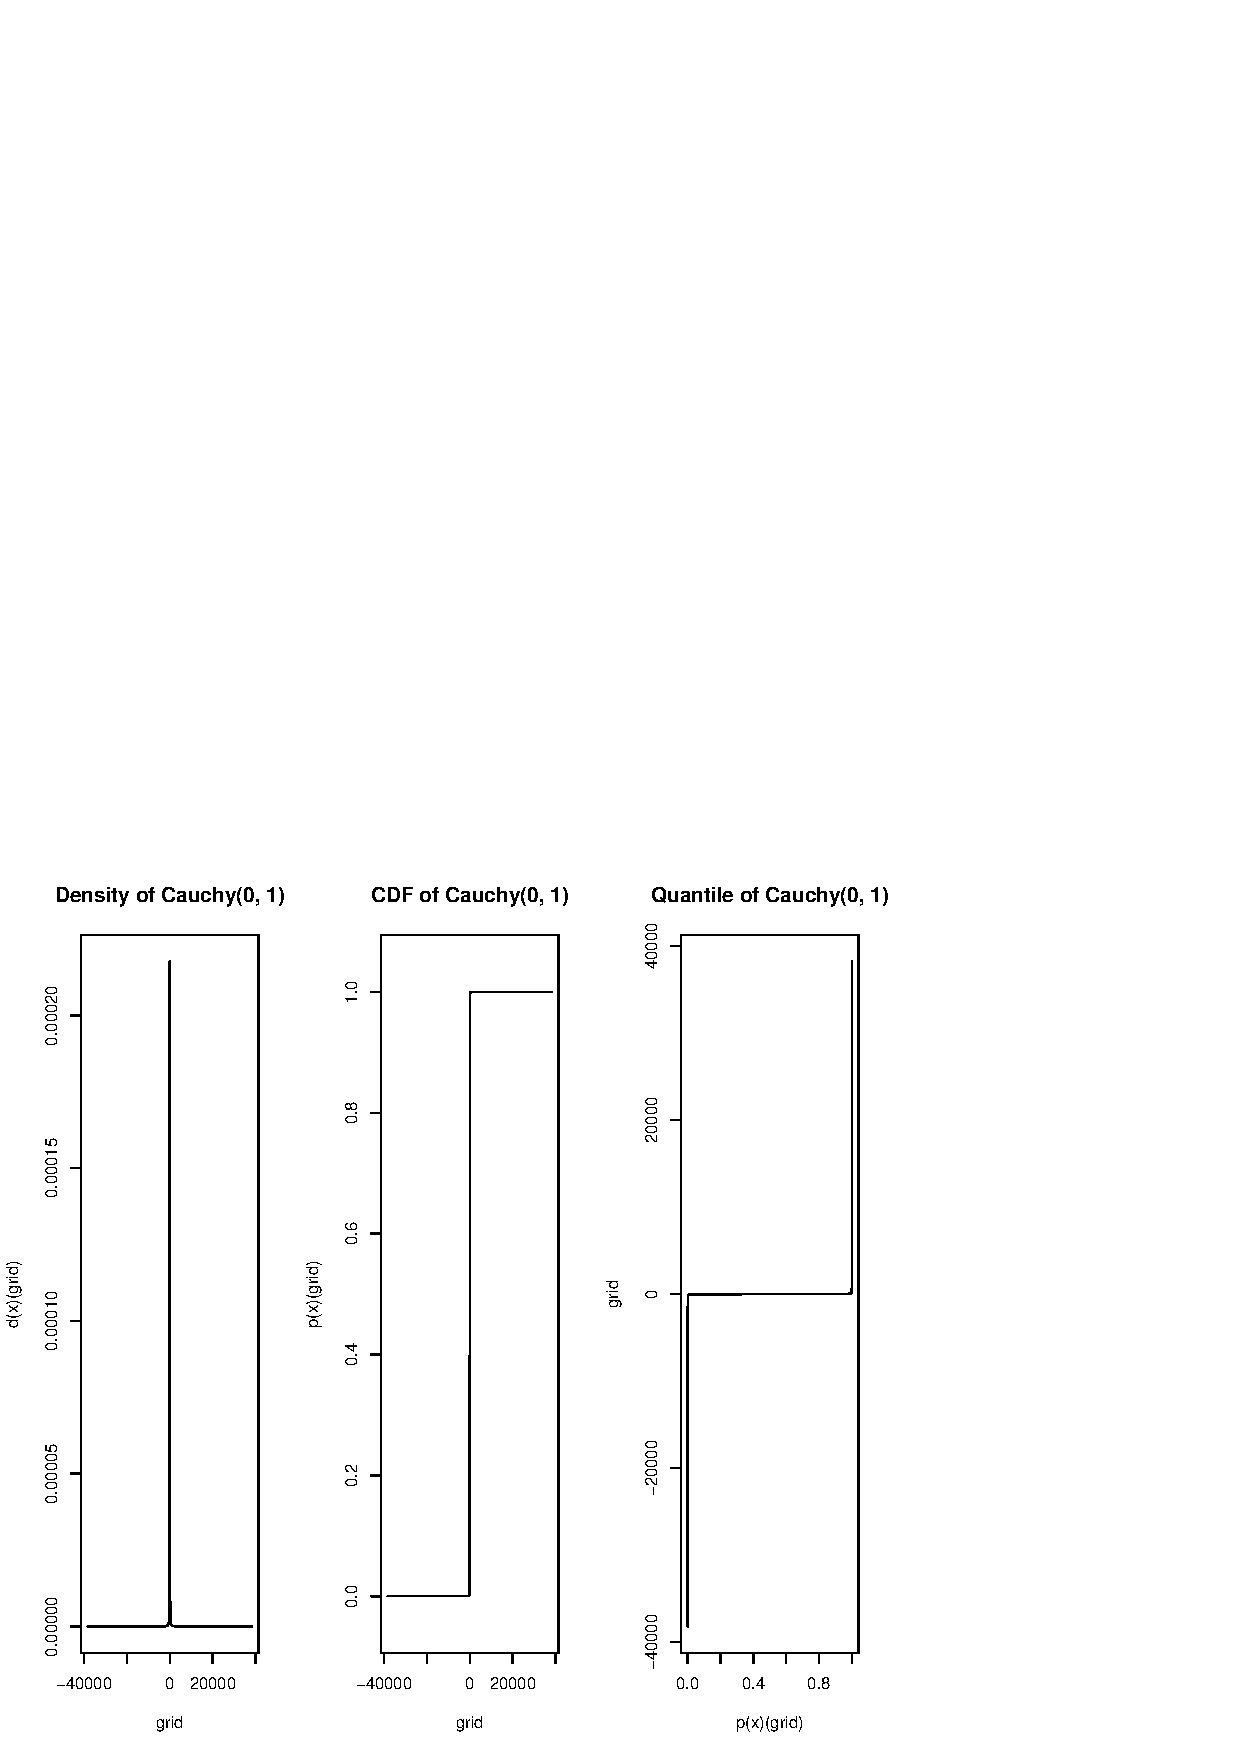
\includegraphics{distr-cauchy1}
\begin{Schunk}
\begin{Sinput}
> plot(Cauchy(), xlim = c(-4, 4))
\end{Sinput}
\end{Schunk}
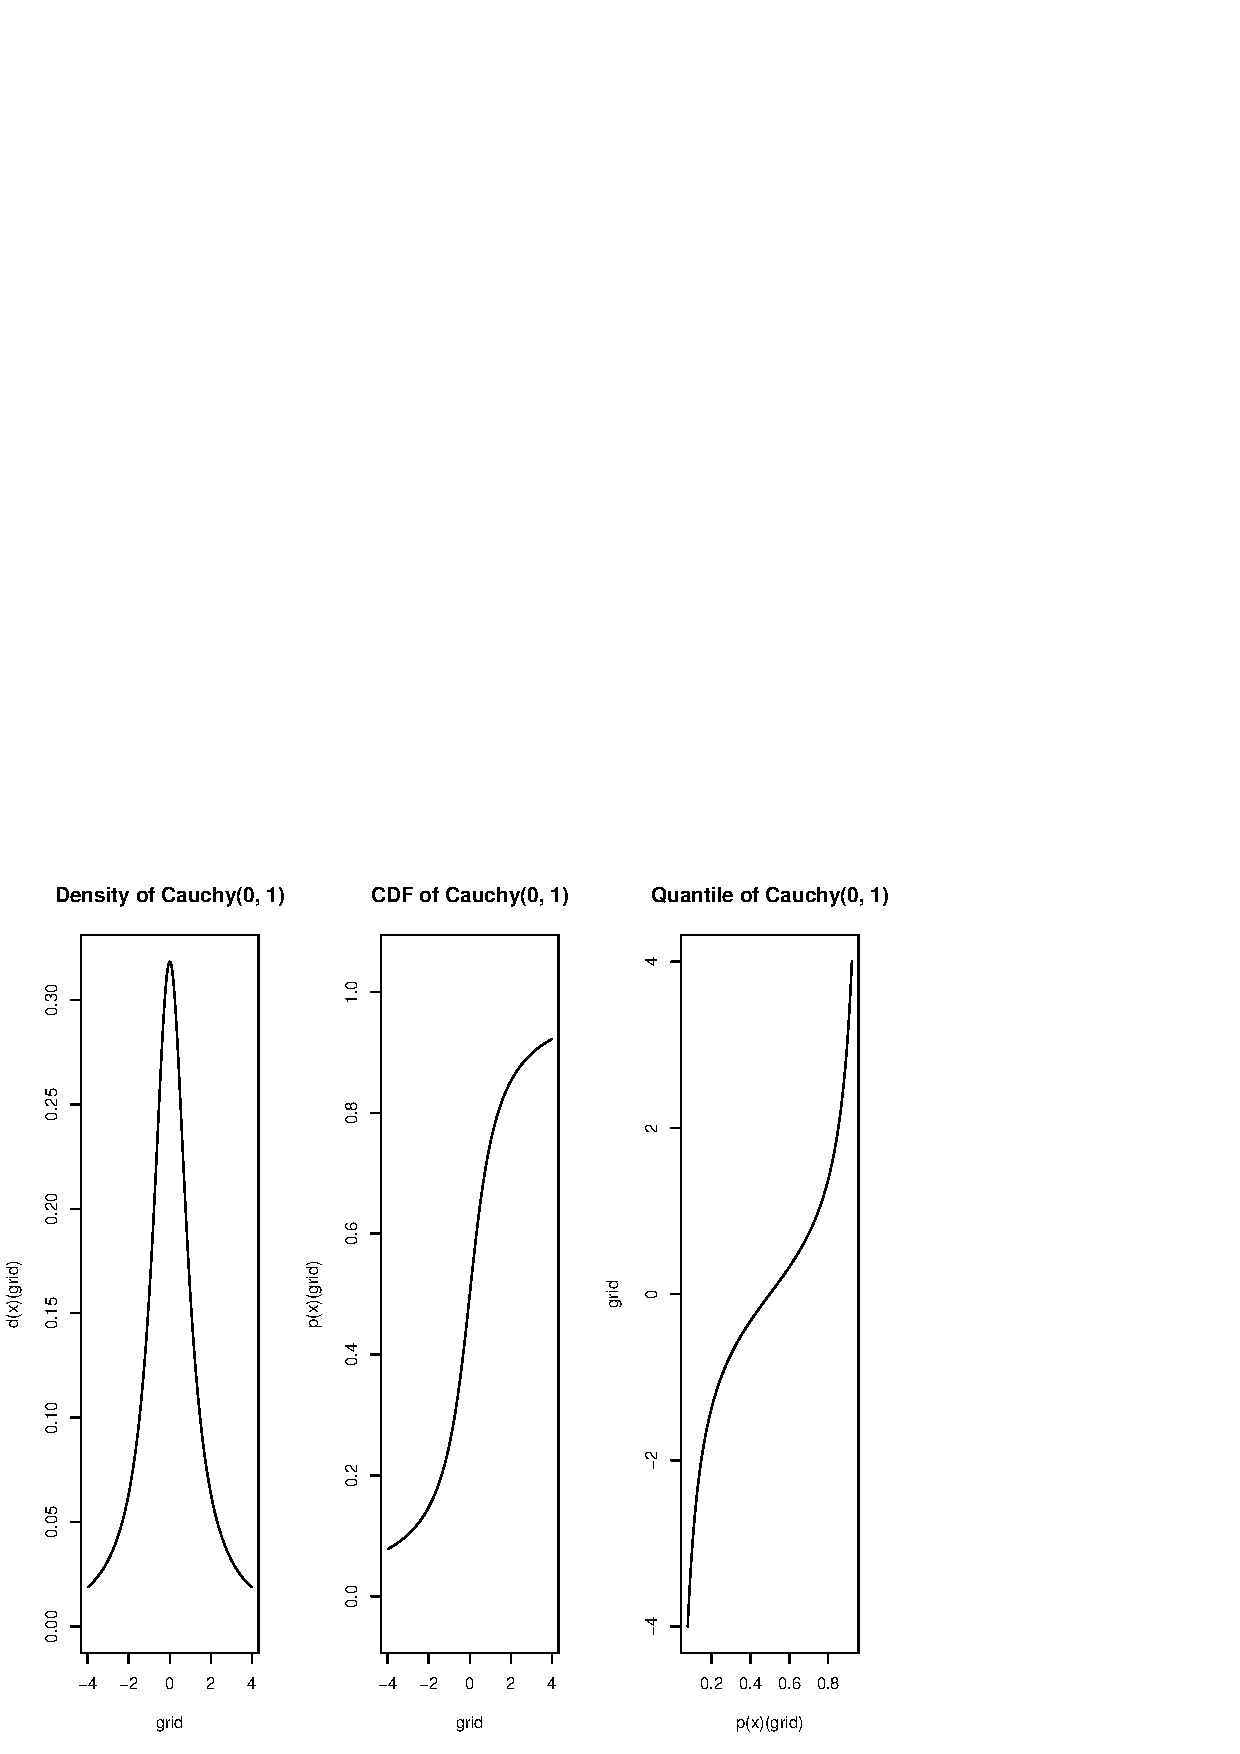
\includegraphics{distr-cauchy2}
\par
For objects of  class \code{Dataclass} ---or of a corresponding subclass---
 \code{plot} plots the sample against the run index and in case  of  \code{ContSimulation} the
 contaminating variables are highlighted by a different color. Additional arguments controlling
 the plot as in the default \code{plot} command may be passed, confer \code{help("plot-methods",package="distrSim")}.
 \par
 For an object of class \code{Evaluation},
\code{plot} yields a boxplot of the results of the evaluation.
For an object of class \code{EvaluationList},
\code{plot} regroups the list according to the different columns/coordinates of the result
of the evaluation; for each such coordinate, a boxplot is generated, containing possibly several procedures,
and, if evaluated at a \code{Contsimulation}, the plots are also grouped into evaluations on ideal and
real data. As for the usual \code{boxplot} function you may pass additional ``\code{plot}-type'' arguments
to this particular \code{plot} method, confer \code{help("plot-methods",package="distrTEst")}. In particular, the \code{plot}-arguments \code{main}
and \code{ylim}, however, may also be transmitted coordinatewise,
i.e.; a vector of the same length as the dimension of the result {\tt resDim} (e.g.\ parameter dimension),
respectively a {\tt 2 x resDim} matrix, or they may be transmitted globally, using the usual {\tt S} recycling
rules.
%\newline??????1

\subsection[Simulation (in package distrSim)]{Simulation (in package \pkg{distrSim})}
%
From version 1.6 on, \code{simulation} is available in package  \pkg{distrSim}.

For the classes \code{Simulation} and \code{ContSimulation}, we normally will
not save the current values of the simulation, as they can easily be reproduced
knowing the values of the other slots of this class.
%
So when declaring a new object of either of the two classes, the slot \code{Data}
will be empty (\code{NULL}).
To fill it with the simulated values, we have to apply the method \code{simulate} to the object.
This has to be redone whenever another slot of the object is changed.
%
To guarantee reproducibility, we use the slot \code{seed}.\\
%
This slot is controlled and set through \href{mailto:pgilbert@bank-banque-canada.ca}{Paul Gilbert's} \pkg{setRNG} package.
By default, \code{seed} is set to \code{setRNG()}, which returns the current ``state'' of the
random number generator (RNG). So the user does not need to specify a value for \code{seed},
and nevertheless may reproduce his samples: He simply uses \code{simulate} to fill the \code{Data} slot.
If the user wants to, he may also set the \code{seed} explicitly via the replacement function
\code{seed()}, but has to take care of the correct format himself, confer the documentation of \code{setRNG}.
One easy way to fill the \code{Data} slot of a simulation \code{X} with ``new'' random numbers is
\begin{Schunk}
\begin{Sinput}
> have.distrSim <- suppressWarnings(require("distrSim"))
> if (have.distrSim) {
+     X <- Simulation()
+     seed(X) <- setRNG()
+     simulate(X)
+ } else {
+     cat("\n functionality not (yet) available; ")
+     cat("you have to install package \"distrSim\" first.\n")
+ }
\end{Sinput}
\end{Schunk}
%
\subsection[Evaluate (in package distrTEst)]{Evaluate (in package \pkg{distrTEst})}\label{evaluate}
%
From version 1.6 on \code{evaluate} is available in  \pkg{distrTEst}.

In an object of class \code{Evaluation}  we store relevant information
about an evaluation of a statistical procedure (estimator/test/predictor)
on an object of class \code{Dataclass}, including the concrete results of
this evaluation. An object of class \code{Evaluation}  is generated by an application
of method \code{evaluate} which takes as arguments an object of class 
\code{Dataclass} and a procedure of type \code{function}. As an example, 
confer Example~\ref{simex}.
For data of class \code{Contsimulation}, the result takes a slightly different,
combining evalations on ideal and real data.
%
\subsection{Is-Relations}
%
By means of \code{setIs}, we have ``told'' {\sf R}  that a distribution object \code{obj} of class
\begin{itemize}
  \item  \code{"Unif"} with  $\code{Min} \doteq 0$ and  $\code{Max} \doteq 1$ also is
   a Beta distribution with parameters \code{shape1 = 1, shape2 = 1}
  \item  \code{"Geom"} also is a negative Binomial distribution with parameters
         \code{size = 1, prob = prob(obj)}
  \item \code{"Cauchy"} with $\code{location} \doteq 0$ and $\code{scale}\doteq 1$ also is a T distribution with parameters
         \code{df = 1, ncp = 0}
  \item \code{"Exp"} also is a Gamma distribution with parameters \code{shape = 1, scale = 1/rate(obj)} and
         a Weibull  distribution with parameters \code{shape = 1, scale = 1/rate(obj)}
  \item \code{"Chisq"} with non-centrality $\code{ncp}\doteq 0$ also is a Gamma distribution with parameters \code{shape = df(obj)/2, scale = 2}
\end{itemize}
%
\subsection{Further methods}
%
When iterating/chaining mathematical operations on a univariate distribution,
generation process of random variables can become clumsy and slow.
To cope with this, we introduce a sort of ``Forget-my-past''-method \code{simplifyr}
that replaces the  chain of mathematical operations in the \code{r}-method by drawing
with replacement from a large sample ($10^{\tt RtoDPQ.e}$) of these.
%
\subsection[Functionals (in package distrEx)]{Functionals (in package \pkg{distrEx})}\label{Functionals}
%
\subsubsection{Expectation}
The most important contribution of package \pkg{distrEx} is a general expectation operator.
In basic statistic courses, the expectation ${\rm E}$ may come as ${\rm E}\,[X]$, ${\rm E}\,[f(X)]$, ${\rm E}\,[X|Y=y]$,
or ${\rm E}\,[f(X)|Y=y]$. Our operator (or in S4-language ``generic function'') \code{E} covers all of
these situtations (or {\it signatures\/}).
\paragraph{default call}
The most frequent call will be \code{E(X)} where \code{X} is an (almost) arbitrary distribution object.
More precisely, if \code{X} is of a specific distribution class like \code{Pois}, it is evaluated exactly
using analytic terms. Else if it is of class \code{DiscreteDistribution} we use a sum over the support of \code{X},
and if it is of class \code{AbscontDistribution} we use numerical integration\footnote{i.e., we first try (really(!): \code{try})
\code{integrate} and if this fails we use Gau{\ss}-Legendre integration according to \cite{NumR:92}, see also
\code{?distrExIntegrate}}; if we only know that {\tt X} is of class \code{UnivariateDistribution} we use Monte-Carlo integration.
This also is the default method in for class \code{MultivariateDistribution}, while for \code{DiscreteMVDistribution} we again use sums.
\paragraph{with a function as argument}
 we proceed just as without: if \code{X} is of class \code{DiscreteDistribution}, we use a sum over the support of \code{X},
and if \code{X} is of class \code{AbscontDistribution} we use numerical integration; else we use Monte-Carlo integration.
\paragraph{in addition: with a condition as argument} we simply use the corresponding \code{d} respective \code{r} slots
with the additional argument \code{cond}.
\paragraph{exact evaluation}
is available for \code{X} of class \code{Beta} (for noncentrality $0$), \code{Binom}, \code{Cauchy}, \code{Chisq},\code{Dirac}, \code{Exp}, \code{Fd}, \code{Gammad},
\code{Geom}, \code{Hyper}, \code{Logis}, \code{Lnorm}, \code{Nbinom}, \code{Norm}, \code{Pois}, \code{Td}, \code{Unif}, \code{Weibull}.
\paragraph{examples} $ \mbox{ }$\newline
\begin{Schunk}
\begin{Sinput}
> have.distrEx <- suppressWarnings(require("distrEx"))
> if (have.distrEx) {
+     D4 <- LMCondDistribution(theta = 1)
+     D4
+     N <- Norm(mean = 2)
+     E(D4, cond = 1)
+     E(D4, cond = 1, useApply = FALSE)
+     E(as(D4, "UnivariateCondDistribution"), cond = 1)
+     E(as(D4, "UnivariateCondDistribution"), cond = 1, useApply = FALSE)
+     E(D4, function(x) {
+         x^2
+     }, cond = 2)
+     E(D4, function(x) {
+         x^2
+     }, cond = 2, useApply = FALSE)
+     E(N, function(x) {
+         x^2
+     })
+     E(as(N, "UnivariateDistribution"), function(x) {
+         x^2
+     }, useApply = FALSE)
+     E(D4, function(x, cond) {
+         cond * x^2
+     }, cond = 2, withCond = TRUE)
+     E(D4, function(x, cond) {
+         cond * x^2
+     }, cond = 2, withCond = TRUE, useApply = FALSE)
+     E(N, function(x) {
+         2 * x^2
+     })
+     E(as(N, "UnivariateDistribution"), function(x) {
+         2 * x^2
+     }, useApply = FALSE)
+ } else {
+     cat("\n functionality not (yet) available; ")
+     cat("you have to install package \"distrEx\" first.\n")
+ }
\end{Sinput}
\begin{Soutput}
[1] 10.00136
\end{Soutput}
\end{Schunk}
%
%
\subsubsection{Variance}
The next-common functional is the variance. In order to keep a unified
notation we will use the same name as for the empirical variance, i.e. \code{var}.
\paragraph{masking \pkg{stats}-method \code{var}}
To cope with the different argument structure of the empirical variance,
i.e. \code{var(x, y = NULL, na.rm = FALSE, use)}  and our functional variance, i.e.
\code{var(x, fun = function(t) {t}, cond, withCond = FALSE, useApply = TRUE, ...)}
we have to mask the original \pkg{stats}-method:
\begin{Schunk}
\begin{Sinput}
> var <- function(x, ...) {
+     dots <- list(...)
+     if (hasArg(y)) 
+         y <- dots$y
+     na.rm <- ifelse(hasArg(na.rm), dots$na.rm, FALSE)
+     if (!hasArg(use)) 
+         use <- ifelse(na.rm, "complete.obs", "all.obs")
+     else use <- dots$use
+     if (hasArg(y)) 
+         stats::var(x = x, y = y, na.rm = na.rm, use)
+     else stats::var(x = x, y = NULL, na.rm = na.rm, use)
+ }
\end{Sinput}
\end{Schunk}
before registering \code{var} as generic function.
Doing so, if the \code{x} (or the first) argument of \code{var}
is not of class \code{UnivariateDistribution}, \code{var} behaves identically to
the \pkg{stats} package
\paragraph{default method} if \code{x} is of class \code{UnivariateDistribution}, \code{var}
just returns the variance of distribution \code{X} --- or of \code{fun(X)} if a function
is passed as argument fun, or, if a condition argument \code{cond} (for $Y=y$),  ${\rm Var}\,[X|Y=y]$ respectively ${\rm Var}\,[f(X)|Y=y]$
--- just as for \code{E}.
\paragraph{exact evaluation} is provided for specific distributions if no function and no condition argument is given:
this is available for \code{X} of class \code{Beta} (for noncentrality $0$), \code{Binom}, \code{Cauchy}, \code{Chisq},\code{Dirac}, \code{Exp}, \code{Fd}, \code{Gammad},
\code{Geom}, \code{Hyper}, \code{Logis}, \code{Lnorm}, \code{Nbinom}, \code{Norm}, \code{Pois}, \code{Unif}, \code{Td}, \code{Weibull}.
\subsubsection{Further functionals}
By the same techniques we provide the following functionals for univariate distributions:
\begin{itemize}
  \item standard deviation: \code{sd}
  \item median: \code{median} (not for function/condition arguments)
  \item median of absolute deviations: \code{mad} (not for function/condition arguments)
  \item interquartile range: \code{IQR} (not for function/condition arguments)
\end{itemize}
%
\subsection[Truncated moments (in package distrEx)]{Truncated moments (in package \pkg{distrEx})}\label{m1df}
%
For Robust Statistics, the first two truncated moments are very useful. These are realized as generic functions \code{m1df} and \code{m2df}:
They use the expectation operator for general univariate distributions, but are overloaded for most specific distributions:
\begin{itemize}
  \item \code{Binom}
  \item \code{Pois}
  \item \code{Norm}
  \item \code{Exp}
  \item \code{Chisq}
\end{itemize}
%
\subsection[Distances (in package distrEx)]{Distances (in package \pkg{distrEx})}\label{Distances}
%
For several purposes like Goodness-of-fit tests or minimum-distance estimators, distances between distributions
are useful. This applies in particular to Robust Statistics. In package \pkg{distrEx}, we provide the follwoing distances:
\begin{itemize}
  \item Kolmogoroff distance
  \item total variation distance
  \item Hellinger distance
  \item convex-contamination ``distance'' (asymmetric!) defined as
  $$
d(Q,P):=\inf\{r>0\,|\, \exists \;\mbox{probability } H:\quad Q=(1-r)P+rH \}
  $$
\end{itemize}
\subsection[Functions for demos (in package distrEx)]{Functions for demos (in package \pkg{distrEx})}\label{Demos}
%
To illustrate the possibilities with packages \pkg{distr} and \pkg{distrEx} we include two major demos, each with
extra code to it

\subsubsection{CLT for arbitrary summand distribution}

By means of our convolution algortithm as well as with the operators \code{E} and \code{sd} an illustration for
the CLT is readily written: \code{illustCLT}; we have particular methods for discrete and absolute continuous distributions.
The user may specify a given summand  distribution, an upper limit for the consecutive sums to be considered and a pause
between the corresponding plots in seconds.

\subsubsection{Deconvolution example}

To illustrate conditional distributions and their implementation in \linebreak[4]\pkg{distrEx}, we consider the following situation:
We consider a signal $X\sim P^X$ which is disturbed by noise $\varepsilon\sim P^\varepsilon$, independent from $X$; in fact we observe
$Y=X+\varepsilon$ and want to reconstruct $X$ by means of $Y$. By means of the generating function \code{PrognCondDistribution}
of package \pkg{distrEx}, for absolutely continuous $P^X, P^\varepsilon$, we may determine the factorized conditional
distribution $P^{X|Y=y}$, and based on this either its (posterior) mode oder (posterior) expectation; also see
\code{demo(Prognose, package="distrEx")}.

\section{Options}\label{options}
\subsection[Options for distr]{Options for \pkg{distr}}
Analogously to the \code{options} command in {\sf R} you may specify a number of
global ``constants'' to be used within the package. These include
\begin{itemize}
  \item \code{DefaultNrFFTGridPointsExponent}: the binary logarithm of the number of grid-points used in FFT ---default $12$
  \item \code{DefaultNrGridPoints}: number of grid-points used for a continuous variable ---default $4096$
  \item \code{DistrResolution}: the finest step length that is permitted for a grid for a discrete variable ---default $1{\rm e-}\!06$
  \item \code{RtoDPQ.e}: For simulational determination of \code{d}, \code{p} and \code{q}, $10^{\rm RtoDPQ.e}$ random variables are
  simulated ---default $5$
  \item \code{TruncQuantile}: to work with compact support, random variables are truncated to their lower/upper
  \code{TruncQuantile}-quantile   ---default $1{\rm e-}\!05$
  \item \code{warningSim}: controls whether a warning issued at printing/showing a \code{Distribution} object the slots of which have been
  filled starting with simulations ---default \code{TRUE}
  \item \code{warningArith}: controls whether a warning issued at printing/showing a \code{Distribution} object produced by arithmetics
  operating on distributions ---default \code{TRUE}
\end{itemize}
All current options may be inspected by \code{distroptions()}  and modified by \linebreak[4] \code{distroptions("<options-name>"=<value>)}.
As \code{options},  \code{distroptions("<options-name>")} returns a list of length $1$ with the value of the corresponding option,
so here, just as \code{getOption},  \code{getdistrOption("<options-name>")} will be preferable, which only returns the value.
%\newline0??????
\subsection[Options for distrEx]{Options for \pkg{distrEx}} \label{distrExoptions}
For the moment we use the function \code{distrExOptions(arg = "missing", value = -1)} to manage some global options for
\pkg{distrEx}, i.e.:\\
\code{distrExOptions()} returns a list of these options,
\code{distrExOptions(arg=x)} returns option \code{x}, and
\code{distrExOptions(arg=x,value=y)} sets the value of option \code{x} to {\tt y}.
Currently, the following options are available:
\begin{itemize}
  \item \code{MCIterations}: number of Monte-Carlo iterations used for crude
          Monte-Carlo integration.
  \item \code{GLIntegrateTruncQuantile}: If \code{integrate} fails and there are
          infinite integration limits, the function \code{GLIntegrate} is
          called inside of \code{distrExIntegrate} with the corresponding
          quantiles  \code{GLIntegrateTruncQuantile} resp.\
          \code{1-GLIntegrateTruncQuantile} as finite integration limits.
  \item \code{GLIntegrateOrder}: The order used for the Gau{\ss{}}-Legendre
          integration inside of \code{distrExIntegrate}.
  \item \code{ElowerTruncQuantile}: The lower limit of integration used inside of
           \code{E} which corresponds to the \code{ElowerTruncQuantile}-quantile.
  \item \code{EupperTruncQuantile}: The upper limit of integration used inside of
           \code{E} which corresponds to the
          \code{(1-ElowerTruncQuantile)}-quantile.
  \item \code{ErelativeTolerance}: The relative tolerance used inside of \code{E} when
          calling \code{distrExIntegrate}.
  \item \code{m1dfLowerTruncQuantile}: The lower limit of integration used inside
           of \code{m1df} which corresponds to the
          \code{m1dfLowerTruncQuantile}-quantile.
  \item \code{m1dfRelativeTolerance}: The relative tolerance used inside of
          \code{m1df} when calling \code{distrExIntegrate}.
  \item \code{m2dfLowerTruncQuantile}: The lower limit of integration used inside
           of \code{m2df} which corresponds to the
          \code{m2dfLowerTruncQuantile}-quantile.
  \item \code{m2dfRelativeTolerance}: The relative tolerance used inside of
          \code{m2df} when calling \code{distrExIntegrate}.
\end{itemize}

We are planning to switch to \code{distroptions}/\code{getdistrOption}-like commands in the next release of this package.
%
\subsection[Options for distrSim]{Options for \pkg{distrSim}}
Just as with to the \code{distroptions}/\code{getdistrOption} commands you may specify certain
global output options to be used within the package with \code{distrSimoptions}/\code{getdistrSimOption}. These include
\begin{itemize}
  \item \code{MaxNumberofPlottedObs} the maximal number of observation plotted in a plot of an object of class \code{Dataclass}; defaults to 4000

  \item \code{MaxNumberofPlottedObsDims}: the maximum number of observations to be plotted in a plot of an object of class \code{Dataclass}
  and descendants; defaults to 6.
  \item \code{MaxNumberofPlottedRuns}: the maximum number of runs to be plotted in a plot of an object of class \code{Dataclass}
  and descendants (one run/panel); defaults to 6.
  \item \code{MaxNumberofSummarizedObsDims}: the maximum number of observations to be summarized of an object of class \code{Dataclass}
  and descendants; defaults to 6.
  \item \code{MaxNumberofSummarizedRuns}: the maximum number of runs to be summarized of an object of class \code{Dataclass}
  and descendants; defaults to 6.
\end{itemize}
%
\subsection[Options for distrTEst]{Options for \pkg{distrTEst}}
Just as with to the \code{distroptions}/\code{getdistrOption} commands you may specify certain
global output options to be used within the package with \code{distrTEstoptions}/\code{getdistrTEstOption}. These include
\begin{itemize}
  \item \code{MaxNumberofPlottedEvaluations}:  the maximal number of evaluations to be plotted
  in a plot of an object of class \code{EvaluationList}; defaults to 6
  \item \code{MaxNumberofPlottedEvaluationDims}: the maximal number of evaluation dimensions to be plotted in a plot of an
         object of class \code{Evaluation}; defaults to 6
  \item \code{MaxNumberofSummarizedEvaluations}: the  maximal number of evaluations to be summarized of an object of class
  \code{EvaluationList}; defaults to 15
  \item \code{MaxNumberofPrintedEvaluations}: the maximal number of evaluations printed of an object of class
  \code{EvaluationList}; defaults to 15
\end{itemize}

%??????1

\section{Startup Messages}
%
For the management of startup messages, from version~1.7, we use package \pkg{startupmsg}:
When loading/attaching packages \pkg{distr}, \pkg{distrEx}, \pkg{distrSim}, or \pkg{distrTEst}
for each package a disclaimer is displayed.

You may suppress these start-up banners/messages completely by setting \linebreak[4]\code{options("StartupBanner"="off")}
somewhere before loading this package by \code{library} or \code{require} in your R-code / R-session.

If option \code{"StartupBanner"} is not defined (default) or setting\linebreak[4]
\code{options("StartupBanner" = NULL)} or %\linebreak[4]
\code{options("StartupBanner" = "complete")}
the complete start-up banner is displayed.

For any other value of option \code{"StartupBanner"} (i.e., not in \linebreak[3]\code{c(NULL, "off", "complete")})
only the version information is displayed.

The same can be achieved by wrapping the \code{library} or \code{require}  call into
either \linebreak[4]\code{onlytypeStartupMessages(<code>, atypes="version")} or \code{suppressStartupMessages(<code>)}.
%

\section[System/version requirements]{System/version requirements, license, etc.\ }
%
\subsection{System requirements}
%
As our package is completely written in {\sf R}, there are no dependencies
on the underlying OS; of course, there is the usual speed gain
possible on recent machines. We have tested our package on a Pentium~II with 233 MHz,
on Pentium~III's with 0.8--2.1 GHz, and on an Athlon with 2.5 GHz giving a reasonable performance.

\subsection{Required version of {\sf R}}
Contrary to the hardware required,
if you want to use \code{library} or \code{require} to use  \pkg{distr} within {\sf R} code,
you need at least {\sf R} Version {\tt 1.8.1},
as we make use of name space operations only available from that version on;
also, the command \code{setClassUnion}, which is used in some sources, is only available from that version on.\\
%
On the other hand, if the package may be pasted in by \code{source}, the code works with {\sf R} from
version {\tt 1.7.0} on ---but without using name-spaces, which is only available from {\tt 1.8.0} on.
Due to some changes in {\sf R} from version {\tt 1.8.1} to {\tt 1.9.0} and from {\tt 1.9.1} to {\tt 2.0.0}, we have to provide different
{\tt zip}/{\tt tar.gz}-Files for these versions.\\
Versions of \pkg{distr} from version number {\tt 1.5} onwards are only
supplied for {\sf R} Version {\tt 2.0.1 patched} and later.
After a reorganization, versions of \pkg{distr} from version number {\tt 1.6} onwards are only
supplied for {\sf R} Version {\tt 2.2.0 patched} and later.


\subsection{Dependencies}
In package \pkg{distrSim}, and conseqently also in package \pkg{distrTEst} we use
\href{mailto:pgilbert@bank-banque-canada.ca}{Paul Gilbert's}  package \pkg{setRNG}
to be installed from \href{http://cran.r-project.org/mirrors.html}{\tt CRAN}
for the control of the seed of the random number generator in our simulation classes.
More precisely, for our version $\le$ {\tt 1.6}  we need his version $<$ {\tt 2006.2-1},
and for our version $\ge$ {\tt 1.7} we need his version $\ge$ {\tt 2006.2-1}.

From package version {\tt 1.7}/{\tt 0.4-3} on, we also need package \pkg{startupmsg}.
also available on \href{http://cran.r-project.org/mirrors.html}{\tt CRAN}.

\subsection{License}
This software is distributed under the terms of the GNU GENERAL
PUBLIC LICENSE Version 2, June 1991, confer\newline
%\href{http://www.gnu.org/copyleft/gpl.html}{\tt http://www.gnu.org/copyleft/gpl.html}
\href{http://www.gnu.org/copyleft/gpl.html}{\footnotesize \tt http://www.gnu.org/copyleft/gpl.html}

\section{Details to the implementation}
\begin{itemize}
\item As the normal distribution is closed under affine transformations, we have overloaded the
corresponding methods. %The same goes for the exponential distribution under scale transformations.
\item For the general convolution algorithm for univariate probability distribution functions/densities by means
of FFT, which we use in the overloaded {\tt "+"}-operator, confer~\cite{K:R:S:04}.
\item Exact convolution methods are implemented for the normal, the Poisson, the binomial
the negative binomial, the Gamma (and the \code{Exp}), and the {$\chi^2$} distribution;
exact formulae for scale transformations for the Exp-/Gamma-distribution
\item Instances of any class transparent to the user are initialized by\linebreak[4] {\tt<classname>([<slotname>=<value>,...])}
where except for class \code{DataClass} in package \pkg{distrSim} all classes have default values for all their slots; in \code{DataClass},
the slot \code{Data} has to be specified.
\item
As suggested in \cite{OOPGent} all slots are accessed and modified by corresponding
accessor- and replacement functions ---templates for which were produced by \code{standardMethods}.

{\bf We strongly discourage the use of the \code{@}-operator to modify
or even access slots \code{r}, \code{d}, \code{p}, and \code{q}, confer
Example~{\ref{destrex}}.}
\end{itemize}
%
\section{A general utility}
%
Following \cite{OOPGent}, the programmer of {\tt S4}-classes should provide
accessor and replacement functions for the inspection/modification of
any newly introduced slot. This can be quite a task when you have a lot of classes/slots.
As these functions all have the same structure, it would be nice
to automatically generate templates for them.
Faced with this problem in developing this package, Thomas Stabla
has written such a utility, \code{standardMethods} ---which the authors
of this package recommend for any developer of {\tt S4}-classes.
For more details, see \code{?standardMethods}.

\section{Odds and Ends}
\subsection[What should be done and what we could do]{What should be done and what we could do ---for version $>$\pkgversion}
\begin{itemize}
\item application of FFT to any univariate distributions ---perhaps also to be controlled
by a parameter/option
\item use the \code{q}-slot applied to \code{runif} in \code{simplifyr} for continuous distributions
\item further exact formulae for binary arithmetic operations like \code{"*"}
\item derivation of a class \code{LatticeDistribution} from \code{DiscreteDistribution} to be able to easily apply FFT
\item redo the initialize- and the math-method for discrete distributions when only slot \code{r} is given
%\item better documentation for method \code{evaluate} / class \code{Evaluation}
%\item adaptation of class \code{Evaluation} / method \code{evaluate} to be more flexible
%\item use of  \code{initialize} in generating functions
\item generating function for new distribution classes to ease inclusion of new distributions
\item goodness of fit tests for distribution-objects
\item use of $\tt \backslash$\code{S4method} in documentation
\item overloading binary operators of group \code{Math2} for independent distributions
\item defining a subgroup of \code{Math2} of invertible binary operators
\item better use of \code{concept} in rd-files
%\item suggestion by \href{mailto:kouros.owzar@duke.edu}{Kouros Owzar}: in case of parameters of dimension $p>1$
%---as in case of ${\cal N}(\mu,\sigma^2)$--- possibility to access/replace that parameter  as a vector
\end{itemize}
\subsection{What should be done but for which we lack the know-how}
\begin{itemize}
  \item multivariate distributions
  \item conditional distributions
  \item copula
\end{itemize}
%
\section{Acknowledgement}
In order to give our acknowledgements their due place
in the manual, we insert them before some rather
extensive presentation of examples, because otherwise
they would probably get lost or overseen by most of the
readers.

We thank Martin M\"achler and Josef Leydold for their
helpful suggestions in conceiving the package.
John Chambers also gave several helpful hints and
insights when responding to our requests concerning the
{\tt S4}-class concept in {\tt r-devel}/ {\tt r-help}.
We got stimulating replies to an RFC on {\tt r-devel} by
Duncan Murdoch and Gregory Warnes.
We also thank Paul Gilbert for drawing our attention to his package
 {\tt setRNG} and making it available as stand-alone version.
In the last few days before the release on {\tt CRAN}, Kurt Hornik and
Uwe Ligges were very kind, helping us to find the clue how to
pass all necessary checks by {\tt R cmd check}.

Last not least a big "thank you" to Torsten Hothorn as editor
of {\tt R-News}, for his patience with our endless versions
until we finally came to a publishable version.
%\input{distrack}
%
\section{Examples}
\subsection{$12$-fold convolution of uniform $(0,1)$ variables}
\begin{footnotesize}
  Code also available under\newline {\href{http://www.uni-bayreuth.de/departments/math/org/mathe7/DISTR/NormApprox.R}%
  {\parbox[t]{12cm}{$\mbox{\hspace{2cm}}${\tt http://www.uni-bayreuth.de/departments/math/org/}\\%
  {$\mbox{\hspace{2cm}}$\hphantom{\tt http:/}{\tt /mathe7/DISTR/NormApprox.R}}}}}\\[2ex]
\end{footnotesize}
\begin{small}
  This example shows how easily we may get the distribution of the sum of $12$
  ${\rm i.i.d.}$ ${\rm ufo}(0,1)$--variables minus $6$--- which was used as a fast generator
  of ${\cal N}(0,1)$--variables in times when evaluations of $\exp$, $\log$, $\sin$ and $\tan$ were expensive, confer
  \cite{Ric:88}, example~C, p.~163. The user should not be confused by expressions  like {\tt U+U}: this {\em does not\/} mean {\tt 2U}
  but rather convolution of two independent identically distributed random variables.
\end{small}
\begin{Schunk}
\begin{Sinput}
> require(distr)
\end{Sinput}
\begin{Soutput}
[1] TRUE
\end{Soutput}
\begin{Sinput}
> N <- Norm(0, 1)
> U <- Unif(0, 1)
> U2 <- U + U
> U4 <- U2 + U2
> U8 <- U4 + U4
> U12 <- U4 + U8
> NormApprox <- U12 - 6
> x <- seq(-4, 4, 0.001)
> opar <- par()
> par(mfrow = c(2, 1))
> plot(x, d(NormApprox)(x), type = "l", xlab = "", ylab = "Density", 
+     main = "Exact and approximated density")
> lines(x, d(N)(x), col = "red")
> legend(-4, d(N)(0), legend = c("NormApprox", "Norm(0,1)"), fill = c("black", 
+     "red"))
> plot(x, d(NormApprox)(x) - d(N)(x), type = "l", xlab = "", ylab = "\"black\" - \"red\"", 
+     col = "darkgreen", main = "Error")
> lines(c(-4, 4), c(0, 0))
> par(opar)
\end{Sinput}
\end{Schunk}
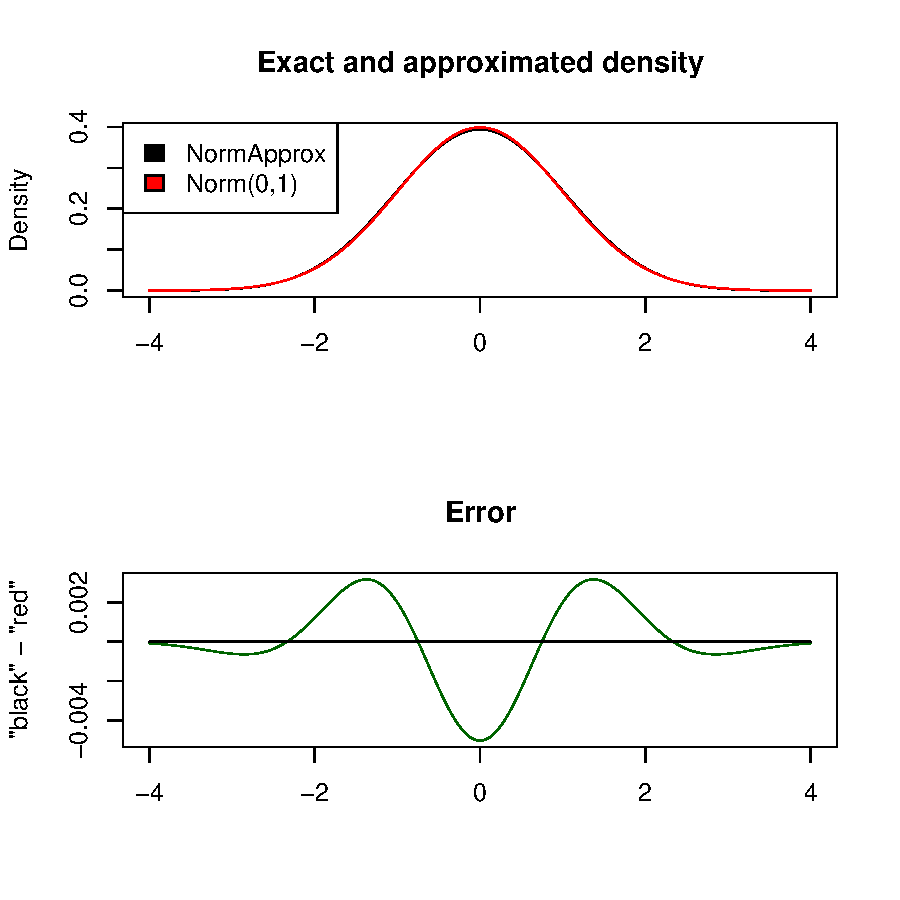
\includegraphics{distr-NormApprox}
\subsection{Comparison of exact convolution to FFT for normal distributions}\label{Convex}
\begin{footnotesize}
  Code also available under\newline \href{http://www.uni-bayreuth.de/departments/math/org/mathe7/DISTR/ConvolutionNormalDistr.R}%
  {\parbox[t]{12cm}{$\mbox{\hspace{2cm}}${\tt http://www.uni-bayreuth.de/departments/math/org/}\\%
  {$\mbox{\hspace{2cm}}$\hphantom{\tt http:/}{\tt /mathe7/DISTR/ConvolutionNormalDistr.R}}}}\\[2ex]
\end{footnotesize}
\begin{small}
  This example illustrates the exactness of the numerical algorithm used to compute the convolution:
  We know that ${\cal L}({\tt A+B})={\cal N}(5,13)$ --- if the second argument of ${\cal N}$ is the variance
\end{small}
\begin{Schunk}
\begin{Sinput}
> require(distr)
\end{Sinput}
\begin{Soutput}
[1] TRUE
\end{Soutput}
\begin{Sinput}
> A <- Norm(mean = 1, sd = 2)
> B <- Norm(mean = 4, sd = 3)
> AB <- A + B
> A1 <- as(A, "AbscontDistribution")
> B1 <- as(B, "AbscontDistribution")
> oldeps <- getdistrOption("TruncQuantile")
> eps <- 1e-08
> distroptions(TruncQuantile = eps)
> AB1 <- A1 + B1
> par(mfrow = c(1, 3))
> low <- q(AB)(1e-15)
> upp <- q(AB)(1 - 1e-15)
> x <- seq(from = low, to = upp, length = 10000)
> plot(x, d(AB)(x), type = "l", lwd = 5)
> lines(x, d(AB1)(x), col = "orange", lwd = 1)
> title("Densities")
> legend(low, d(AB)(5), legend = c("exact", "FFT"), fill = c("black", 
+     "orange"))
> plot(x, p(AB)(x), type = "l", lwd = 5)
> lines(x, p(AB1)(x), col = "orange", lwd = 1)
> title("Cumulative distribution functions")
> legend(low, 1, legend = c("exact", "FFT"), fill = c("black", 
+     "orange"))
> x <- seq(from = eps, to = 1 - eps, length = 1000)
> plot(x, q(AB)(x), type = "l", lwd = 5)
> lines(x, q(AB1)(x), col = "orange", lwd = 1)
> title("Quantile functions")
> legend(0, q(AB)(1 - eps), legend = c("exact", "FFT"), fill = c("black", 
+     "orange"))
> total.var <- function(z, N1, N2) {
+     0.5 * abs(d(N1)(z) - d(N2)(z))
+ }
> dv <- integrate(total.var, lower = -Inf, upper = Inf, rel.tol = 1e-08, 
+     N1 = AB, N2 = AB1)
> cat("Total variation distance of densities:\t")
\end{Sinput}
\begin{Soutput}
Total variation distance of densities:	
\end{Soutput}
\begin{Sinput}
> print(dv)
\end{Sinput}
\begin{Soutput}
4.250016e-07 with absolute error < 1.8e-09
\end{Soutput}
\begin{Sinput}
> z <- r(Unif(Min = low, Max = upp))(1e+05)
> dk <- max(abs(p(AB)(z) - p(AB1)(z)))
> cat("Kolmogorov distance of cdfs:\t", dk, "\n")
\end{Sinput}
\begin{Soutput}
Kolmogorov distance of cdfs:	 2.028470e-07 
\end{Soutput}
\begin{Sinput}
> distroptions(TruncQuantile = oldeps)
\end{Sinput}
\end{Schunk}
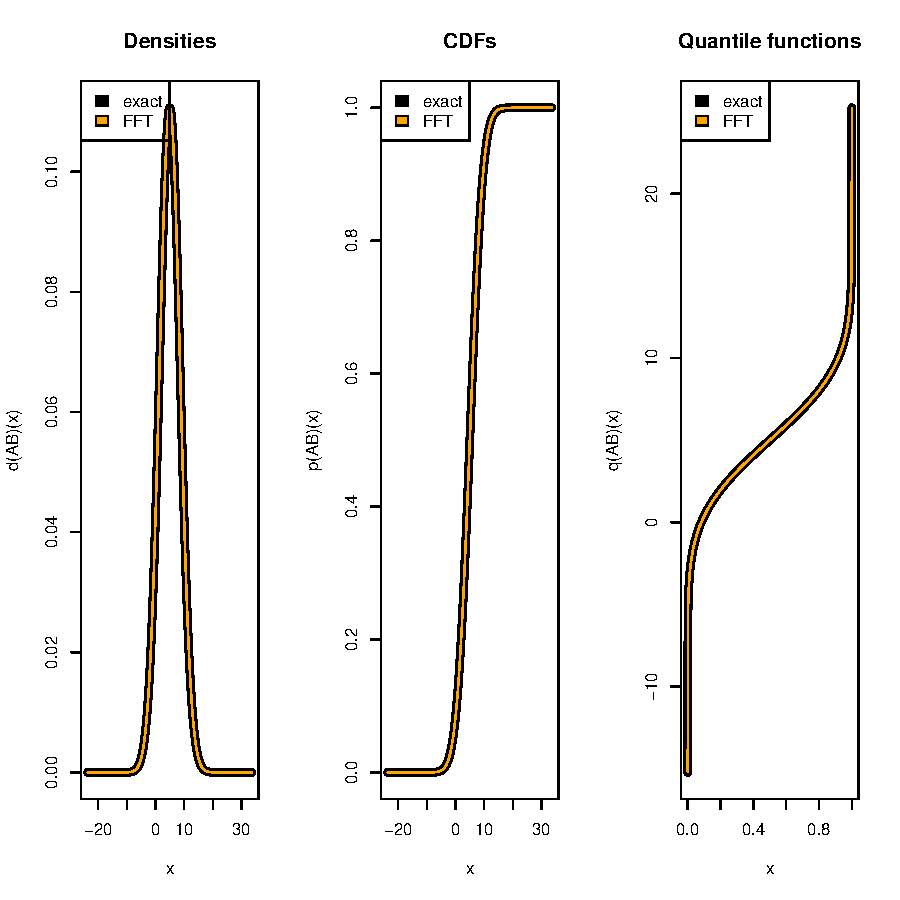
\includegraphics{distr-ConvolutionNormalDistr}
\subsection{Comparison of FFT to {\tt RtoDPQ}}\label{compex}
\begin{footnotesize}
  Code also available under\newline \href{http://www.uni-bayreuth.de/departments/math/org/mathe7/DISTR/ComparisonFFTandRtoDPQ.R}%
  {\parbox[t]{12cm}{$\mbox{\hspace{2cm}}${\tt http://www.uni-bayreuth.de/departments/math/org/}\\%
  {$\mbox{\hspace{2cm}}$\hphantom{\tt http:/}{\tt /mathe7/DISTR/ComparisonFFTandRtoDPQ.R}}}}\\[2ex]
\end{footnotesize}
\begin{small}
  This example illustrates the exactness (or rather not--so--exactness) of the simulational default algorithm used to compute
  the distribution of transformations of group {\tt math}.
\end{small}
\begin{Schunk}
\begin{Sinput}
> require(distr)
\end{Sinput}
\begin{Soutput}
[1] TRUE
\end{Soutput}
\begin{Sinput}
> N1 <- Norm(0, 3)
> N2 <- Norm(0, 4)
> rnew1 <- function(n) r(N1)(n) + r(N2)(n)
> X <- N1 + N2
> Y <- N1 + as(N2, "AbscontDistribution")
> Z <- new("AbscontDistribution", r = rnew1)
> x <- seq(-15, 15, 0.01)
> plot(x, d(X)(x), type = "l", lwd = 3, xlab = "", ylab = "density", 
+     main = "Comparison 1", col = "black")
> lines(x, d(Y)(x), col = "yellow")
> lines(x, d(Z)(x), col = "red")
> legend(-15, d(X)(0), legend = c("Exact", "FFT-Approximation", 
+     "RtoDQP-Approximation"), fill = c("black", "yellow", "red"))
> B <- Binom(size = 6, prob = 0.5) * 10
> N <- Norm()
> rnew2 <- function(n) r(B)(n) + r(N)(n)
> Y <- B + N
> Z <- new("AbscontDistribution", r = rnew2)
> x <- seq(-5, 65, 0.01)
> plot(x, d(Y)(x), type = "l", xlab = "", ylab = "density", main = "Comparison 2", 
+     col = "black")
> lines(x, d(Z)(x), col = "red")
> legend(-5, d(Y)(30), legend = c("Exact", "RtoDQP-Approximation"), 
+     fill = c("black", "red"))
\end{Sinput}
\end{Schunk}
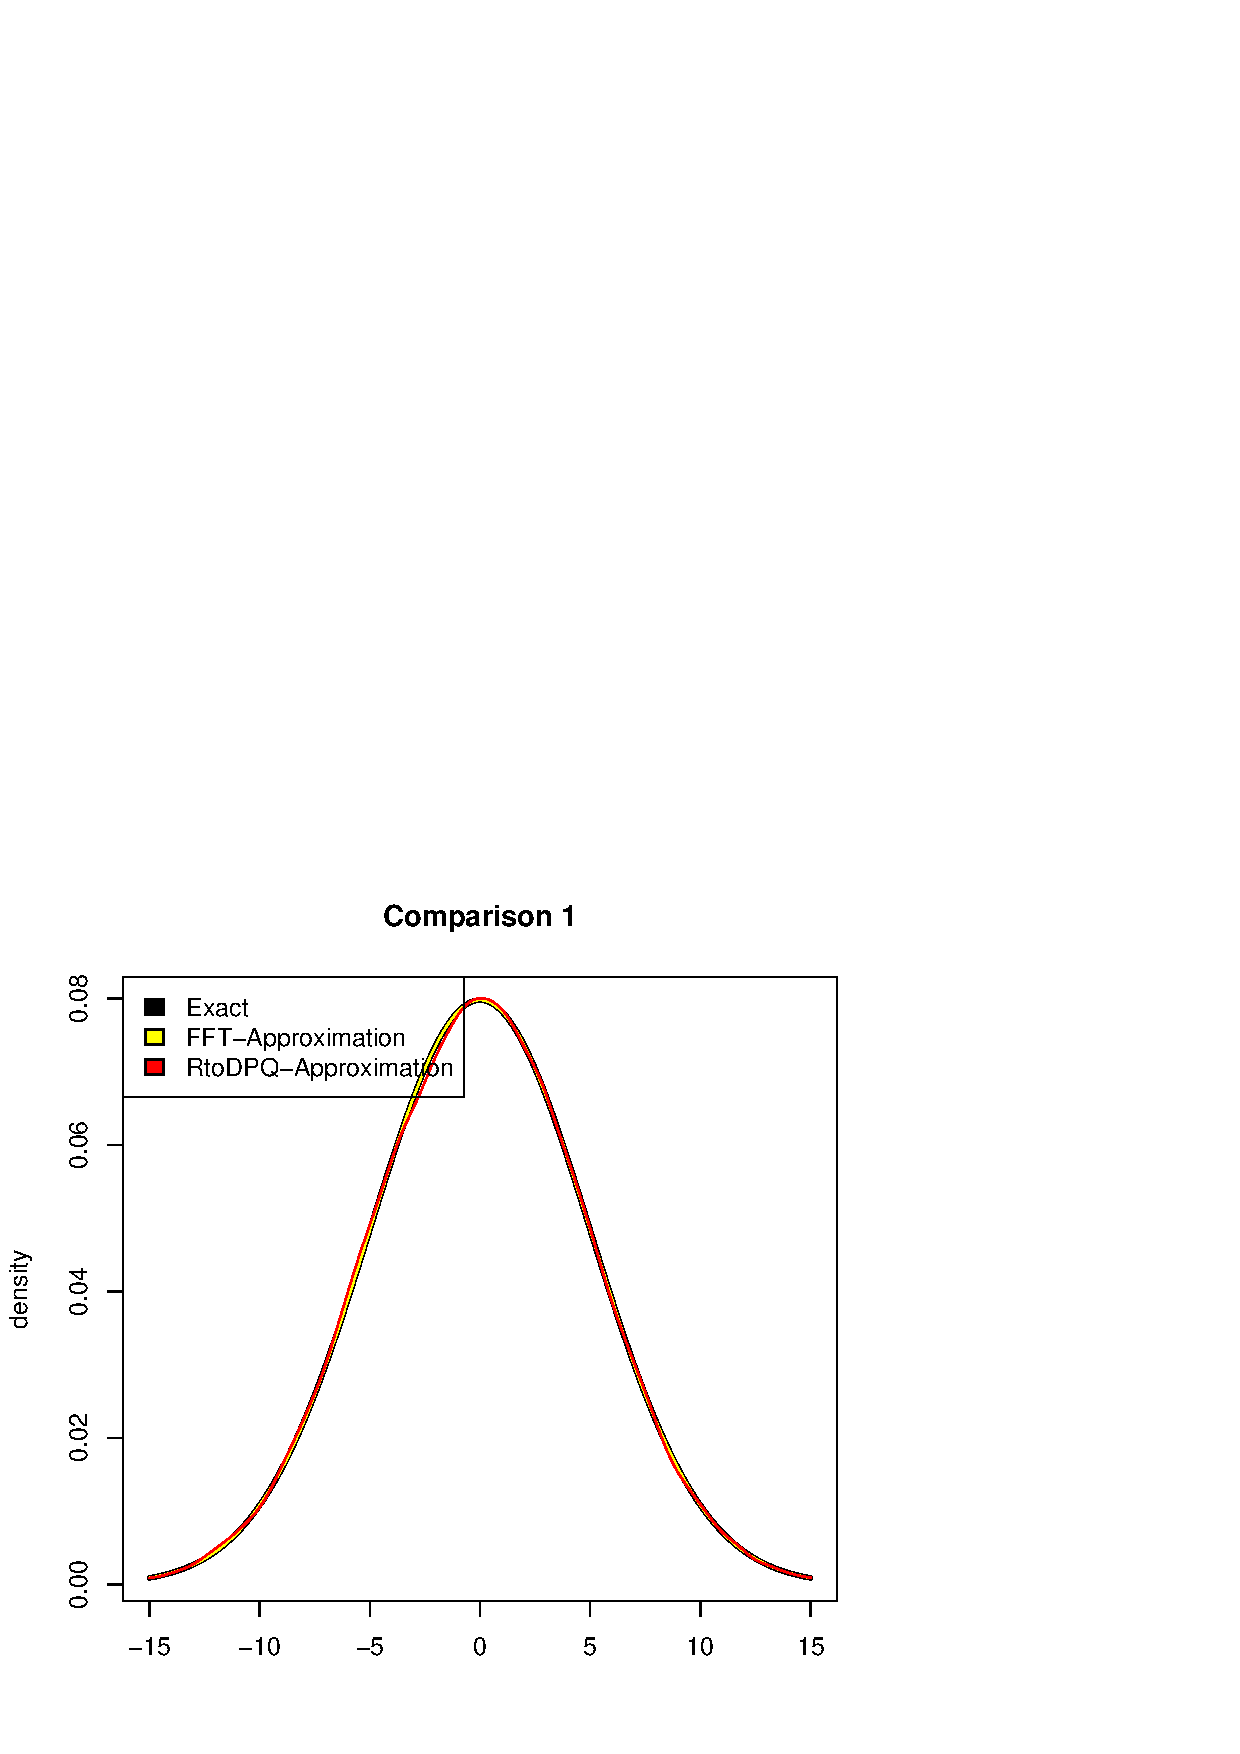
\includegraphics{distr-ComparisonFFTandRtoDPQ}
\subsection{Comparison of exact and approximate stationary regressor distribution}\label{statex}
\begin{footnotesize}
  Code also available under\newline \href{http://www.uni-bayreuth.de/departments/math/org/mathe7/DISTR/StationaryRegressorDistr.R}%
  {\parbox[t]{12cm}{$\mbox{\hspace{2cm}}${\tt http://www.uni-bayreuth.de/departments/math/org/}\\%
  {$\mbox{\hspace{2cm}}$\hphantom{\tt http:/}{\tt /mathe7/DISTR/StationaryRegressorDistr.R}}}}\\[2ex]
\end{footnotesize}
\begin{small}
  Another illustration for the use of package {\tt "distr"}.
  In case of a stationary AR(1)--model, for non--normal innovation distribution, the stationary distribution of
  the observations must be approximated by finite convolutions. That these approximations give fairly good results for
  approximations down to small orders is exemplified by the Gaussian case where we may compare the approximation to
  the exact stationary distribution.
\end{small}
\begin{Schunk}
\begin{Sinput}
> require(distr)
\end{Sinput}
\begin{Soutput}
[1] TRUE
\end{Soutput}
\begin{Sinput}
> phi <- 0.5
> V <- as(Norm(), "AbscontDistribution")
> oldeps <- getdistrOption("TruncQuantile")
> eps <- 1e-08
> distroptions(TruncQuantile = eps)
> H <- V
> n <- 15
> for (i in 1:n) {
+     Vi <- phi^i * V
+     H <- H + Vi
+ }
> X <- Norm(sd = sqrt(1/(1 - phi^2)))
> par(mfrow = c(1, 3))
> low <- q(X)(1e-15)
> upp <- q(X)(1 - 1e-15)
> x <- seq(from = low, to = upp, length = 10000)
> plot(x, d(X)(x), type = "l", lwd = 5)
> lines(x, d(H)(x), col = "orange", lwd = 1)
> title("Densities")
> legend(low, d(X)(0), legend = c("exact", "FFT"), fill = c("black", 
+     "orange"))
> plot(x, p(X)(x), type = "l", lwd = 5)
> lines(x, p(H)(x), col = "orange", lwd = 1)
> title("Cumulative distribution functions")
> legend(low, 1, legend = c("exact", "FFT"), fill = c("black", 
+     "orange"))
> x <- seq(from = eps, to = 1 - eps, length = 1000)
> plot(x, q(X)(x), type = "l", lwd = 5)
> lines(x, q(H)(x), col = "orange", lwd = 1)
> title("Quantile functions")
> legend(0, q(X)(1 - eps), legend = c("exact", "FFT"), fill = c("black", 
+     "orange"))
> total.var <- function(z, N1, N2) {
+     0.5 * abs(d(N1)(z) - d(N2)(z))
+ }
> dv <- integrate(total.var, lower = -Inf, upper = Inf, rel.tol = 1e-05, 
+     N1 = X, N2 = H)
> cat("Total variation distance of densities:\t")
\end{Sinput}
\begin{Soutput}
Total variation distance of densities:	
\end{Soutput}
\begin{Sinput}
> print(dv)
\end{Sinput}
\begin{Soutput}
9.100439e-06 with absolute error < 6.4e-06
\end{Soutput}
\begin{Sinput}
> z <- r(Unif(Min = low, Max = upp))(1e+05)
> dk <- max(abs(p(X)(z) - p(H)(z)))
> cat("Kolmogorov distance of cdfs:\t", dk, "\n")
\end{Sinput}
\begin{Soutput}
Kolmogorov distance of cdfs:	 4.30419e-06 
\end{Soutput}
\begin{Sinput}
> distroptions(TruncQuantile = oldeps)
\end{Sinput}
\end{Schunk}
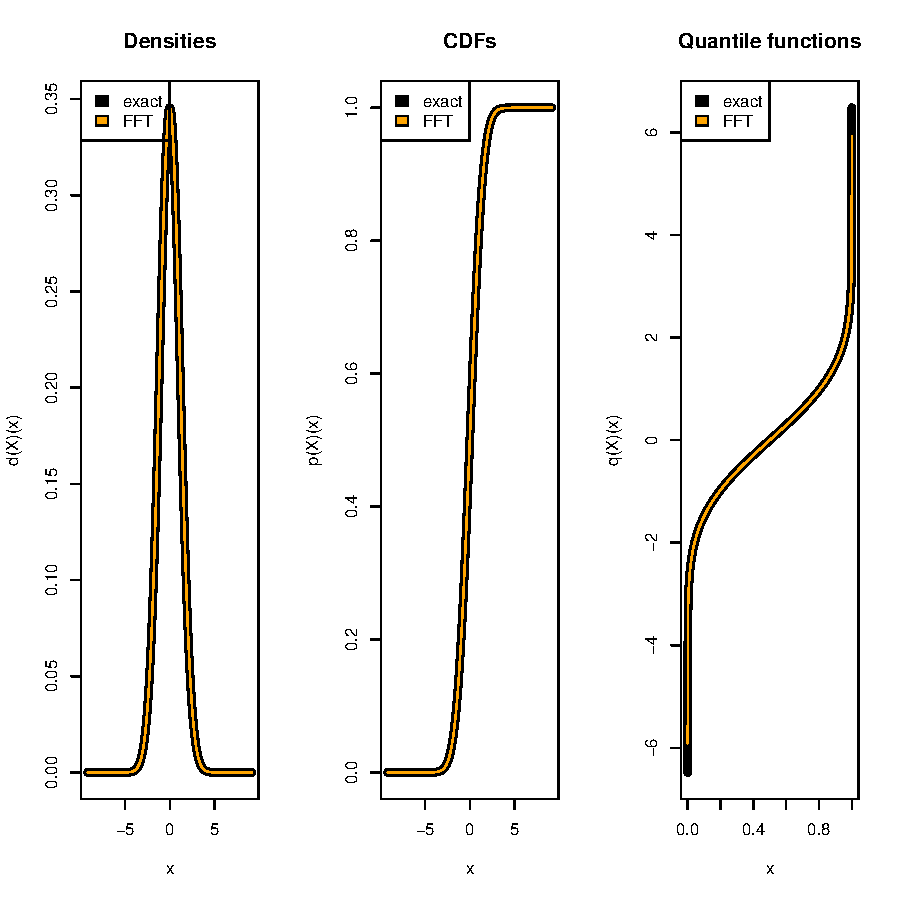
\includegraphics{distr-StationaryRegressorDistr}
\subsection{Truncation and Huberization/winsorization}\label{truncex}
\begin{footnotesize}
  Code also available under\newline \href{http://www.uni-bayreuth.de/departments/math/org/mathe7/DISTR/huberize.R}%
    {\parbox[t]{12cm}{$\mbox{\hspace{2cm}}${\tt http://www.uni-bayreuth.de/departments/math/org/}\\%
  {$\mbox{\hspace{2cm}}$\hphantom{\tt http:/}{\tt /mathe7/DISTR/huberize.R}}}}\\[2ex]
\href{http://www.uni-bayreuth.de/departments/math/org/mathe7/DISTR/truncate.R}%
    {\parbox[t]{12cm}{$\mbox{\hspace{2cm}}${\tt http://www.uni-bayreuth.de/departments/math/org/}\\%
    {$\mbox{\hspace{2cm}}$\hphantom{\tt http:/}{\tt /mathe7/DISTR/truncate.R}}}}\\[2ex]
\end{footnotesize}
\begin{small}
The operations of truncation and Huberization play a crucial role in Robust Statistics, but also
arise in many other contexts like censoring etc; they may now be formulated quite generally as shown
in this example. With the slots {\tt d}, {\tt p} and {\tt q} of class {\tt UnivariateDistribution} being
{\tt OptionalFunction} from version {\tt 1.4} on, it would be no problem to return a corresponding
distribution object now.
\end{small}
\begin{Schunk}
\begin{Sinput}
> require(distr)
\end{Sinput}
\begin{Soutput}
[1] TRUE
\end{Soutput}
\begin{Sinput}
> if (!isGeneric("Huberize")) setGeneric("Huberize", function(object, 
+     lower, upper) standardGeneric("Huberize"))
\end{Sinput}
\begin{Soutput}
[1] "Huberize"
\end{Soutput}
\begin{Sinput}
> setMethod("Huberize", signature(object = "AbscontDistribution", 
+     lower = "numeric", upper = "numeric"), function(object, lower, 
+     upper) {
+     rnew = function(n) {
+         rn = r(object)(n)
+         ifelse(rn < lower, lower, ifelse(rn >= upper, upper, 
+             rn))
+     }
+     pnew = function(x) ifelse(x < lower, 0, ifelse(x >= upper, 
+         1, p(object)(x)))
+     plower = p(object)(lower)
+     pupper = p(object)(upper)
+     qnew = function(x) ifelse(x < plower, ifelse(x < 0, NA, -Inf), 
+         ifelse(x >= pupper, ifelse(x > 1, NA, upper), q(object)(x)))
+     new("UnivariateDistribution", r = rnew, p = pnew, q = qnew, 
+         d = NULL)
+ })
\end{Sinput}
\begin{Soutput}
[1] "Huberize"
\end{Soutput}
\begin{Sinput}
> N = Norm()
> HN = Huberize(N, -0.5, 1)
> r(HN)(10)
\end{Sinput}
\begin{Soutput}
 [1]  1.0000000 -0.5000000  0.2154488  1.0000000  0.6802175 -0.5000000
 [7] -0.5000000  1.0000000  0.2453647  0.5290800
\end{Soutput}
\begin{Sinput}
> oldpar = par()
> par(mfrow = c(1, 2))
> x = seq(-1.5, 1.5, length = 1000)
> plot(x, p(HN)(x), type = "l", lwd = 5, ylab = "CDF")
> lines(x, p(N)(x), lwd = 2, col = "red")
> legend(-1.5, 1, legend = c("N(0,1)", "N(0,1) huberized"), fill = c("red", 
+     "black"))
> x = seq(0, 1, length = 1000)
> plot(x, q(HN)(x), type = "l", lwd = 5, ylab = "Quantiles", ylim = c(-2.5, 
+     3))
> lines(x, q(N)(x), lwd = 2, col = "red")
> legend(0, 3, legend = c("N(0,1)", "N(0,1) huberized"), fill = c("red", 
+     "black"))
> par(oldpar)
\end{Sinput}
\end{Schunk}
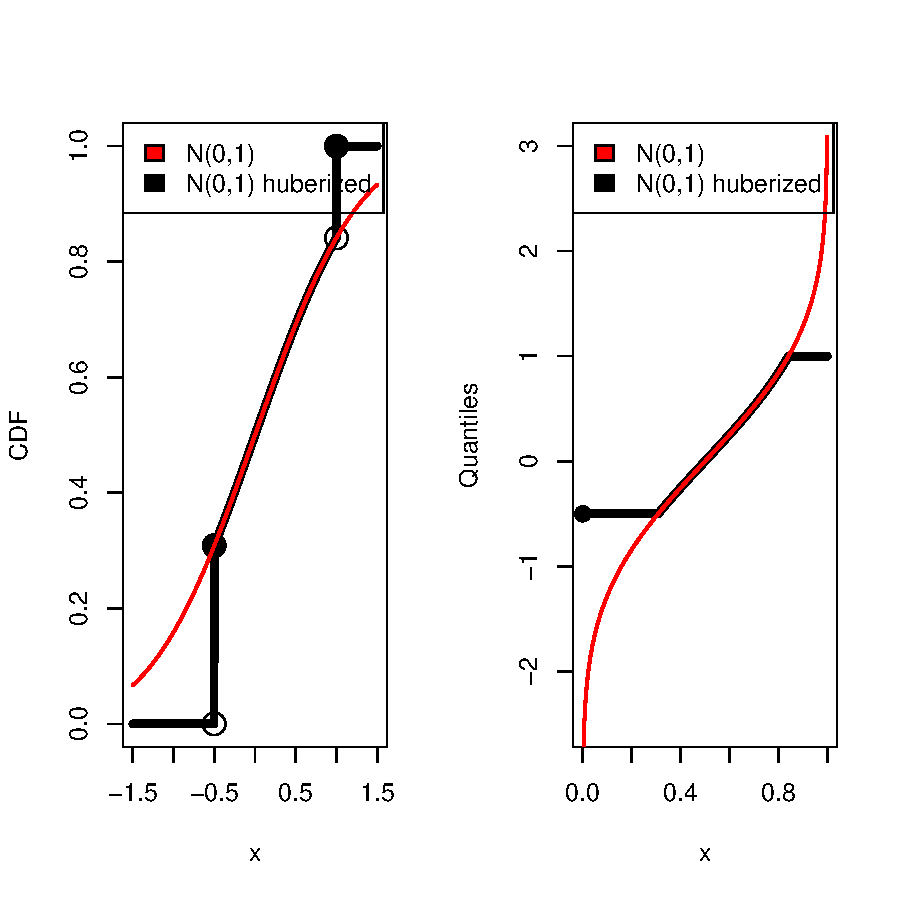
\includegraphics{distr-huberize}
\begin{Schunk}
\begin{Sinput}
> require(distr)
\end{Sinput}
\begin{Soutput}
[1] TRUE
\end{Soutput}
\begin{Sinput}
> if (!isGeneric("Truncate")) setGeneric("Truncate", function(object, 
+     lower, upper) standardGeneric("Truncate"))
\end{Sinput}
\begin{Soutput}
[1] "Truncate"
\end{Soutput}
\begin{Sinput}
> setMethod("Truncate", signature(object = "AbscontDistribution", 
+     lower = "numeric", upper = "numeric"), function(object, lower, 
+     upper) {
+     rnew = function(n) {
+         rn = r(object)(n)
+         while (TRUE) {
+             rn[rn < lower] = NA
+             rn[rn > upper] = NA
+             index = is.na(rn)
+             if (!(any(index))) 
+                 break
+             rn[index] = r(object)(sum(index))
+         }
+         rn
+     }
+     plower = p(object)(lower)
+     pupper = p(object)(upper)
+     pnew = function(x) ifelse(x < lower, 0, ifelse(x >= upper, 
+         1, (p(object)(x) - plower)/(pupper - plower)))
+     lostmass = plower + 1 - pupper
+     dnew = function(x) ifelse(x < lower, 0, ifelse(x >= upper, 
+         0, d(object)(x)/(1 - lostmass)))
+     qfun1 <- function(x) {
+         if (x == 0) 
+             return(lower)
+         if (x == 1) 
+             return(upper)
+         fun <- function(t) pnew(t) - x
+         uniroot(fun, interval = c(lower, upper))$root
+     }
+     qfun2 <- function(x) sapply(x, qfun1)
+     return(new("AbscontDistribution", r = rnew, d = dnew, p = pnew, 
+         q = qfun2))
+ })
\end{Sinput}
\begin{Soutput}
[1] "Truncate"
\end{Soutput}
\begin{Sinput}
> N = Norm()
> Z = Truncate(N, -0.5, 1)
> plot(Z)
> r(Z)(10)
\end{Sinput}
\begin{Soutput}
 [1] -0.26004404 -0.20930077  0.42901044  0.20736589 -0.32304838  0.02591731
 [7] -0.16227450  0.17318232  0.58873571  0.78461899
\end{Soutput}
\begin{Sinput}
> oldpar = par()
> par(mfrow = c(1, 2))
> x = seq(-1.5, 1.5, length = 1000)
> plot(x, p(Z)(x), type = "l", lwd = 5, xlab = "", ylab = "CDF")
> lines(x, p(N)(x), lwd = 2, col = "red")
> legend(-1.5, 1, legend = c("N(0,1)", "N(0,1) truncated"), fill = c("red", 
+     "black"))
> x = seq(-1.5, 1.5, length = 1000)
> plot(x, d(Z)(x), type = "l", lwd = 5, xlab = "", ylab = "density")
> lines(x, d(N)(x), lwd = 2, col = "red")
> legend(-1.5, 0.7, legend = c("N(0,1)", "N(0,1) truncated"), fill = c("red", 
+     "black"))
> par(oldpar)
\end{Sinput}
\end{Schunk}
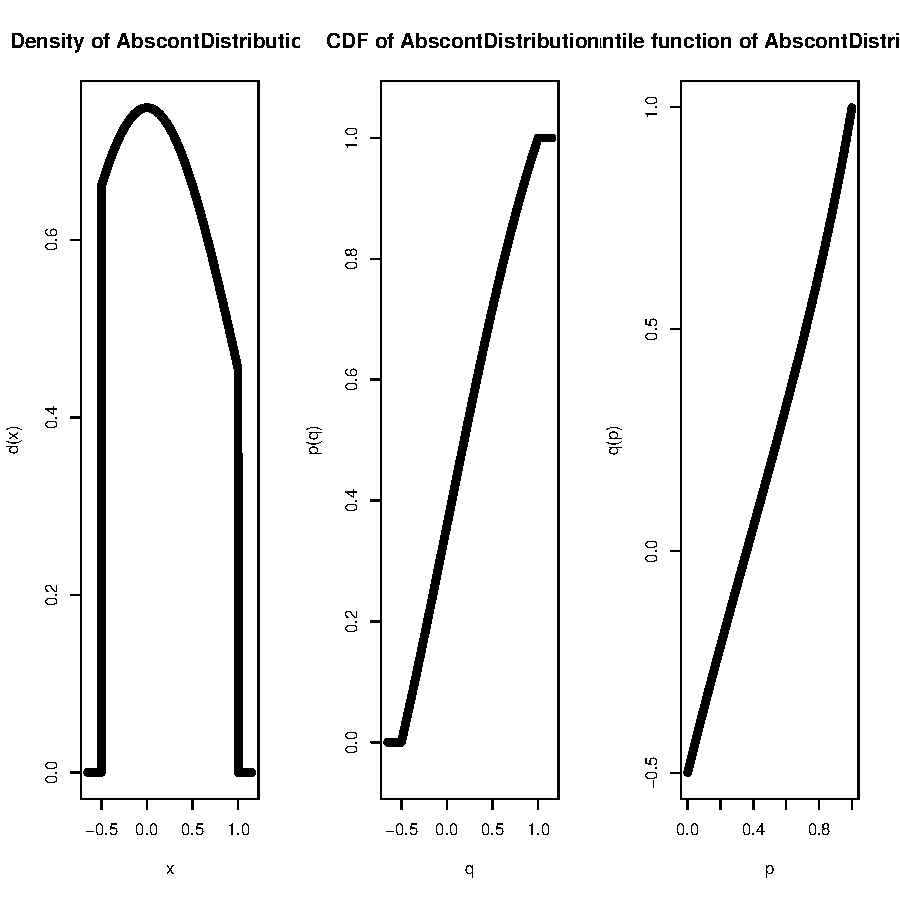
\includegraphics{distr-truncate}
\subsection{Distribution of minimum and maximum of two independent random variables}\label{minmaxex}
\begin{footnotesize}
  Code also available under\newline \href{http://www.uni-bayreuth.de/departments/math/org/mathe7/DISTR/minandmax.R}%
  {\parbox[t]{12cm}{$\mbox{\hspace{2cm}}${\tt http://www.uni-bayreuth.de/departments/math/org/}\\%
  {$\mbox{\hspace{2cm}}$\hphantom{\tt http:/}{\tt /mathe7/DISTR/minandmax.R}}}}\\[2ex]
\end{footnotesize}
\begin{small}
As in the preceding example, we illustrate the use of package {\tt "distr"} by making available
widely necessary operations: Minimum and maximum of two independent random variables.
\end{small}
\begin{Schunk}
\begin{Sinput}
> require(distr)
\end{Sinput}
\begin{Soutput}
[1] TRUE
\end{Soutput}
\begin{Sinput}
> if (!isGeneric("Minimum")) setGeneric("Minimum", function(e1, 
+     e2) standardGeneric("Minimum"))
\end{Sinput}
\begin{Soutput}
[1] "Minimum"
\end{Soutput}
\begin{Sinput}
> setMethod("Minimum", signature(e1 = "AbscontDistribution", e2 = "AbscontDistribution"), 
+     function(e1, e2) {
+         rnew <- function(n) {
+             rn1 <- r(e1)(n)
+             rn2 <- r(e2)(n)
+             ifelse(rn1 < rn2, rn1, rn2)
+         }
+         pnew <- function(x) {
+             p1 <- p(e1)(x)
+             p2 <- p(e2)(x)
+             p1 + p2 - p1 * p2
+         }
+         dnew <- function(x) {
+             d1 <- d(e1)(x)
+             d2 <- d(e2)(x)
+             p1 <- p(e1)(x)
+             p2 <- p(e2)(x)
+             d1 + d2 - d1 * p2 - p1 * d2
+         }
+         lower1 <- q(e1)(0)
+         lower2 <- q(e2)(0)
+         upper1 <- q(e1)(1)
+         upper2 <- q(e2)(1)
+         lower <- min(lower1, lower2)
+         upper <- min(upper1, upper2)
+         maxquantile = min(q(e1)(1 - 1e-06), q(e2)(1 - 1e-06))
+         minquantile = min(q(e1)(1e-06), q(e2)(1e-06))
+         qfun1 <- function(x) {
+             if (x == 0) 
+                 return(lower)
+             if (x == 1) 
+                 return(upper)
+             fun <- function(t) pnew(t) - x
+             uniroot(fun, interval = c(maxquantile, minquantile))$root
+         }
+         qfun2 <- function(x) sapply(x, qfun1)
+         return(new("AbscontDistribution", r = rnew, d = dnew, 
+             p = pnew, q = qfun2))
+     })
\end{Sinput}
\begin{Soutput}
[1] "Minimum"
\end{Soutput}
\begin{Sinput}
> if (!isGeneric("Maximum")) setGeneric("Maximum", function(e1, 
+     e2) standardGeneric("Maximum"))
\end{Sinput}
\begin{Soutput}
[1] "Maximum"
\end{Soutput}
\begin{Sinput}
> setMethod("Maximum", signature(e1 = "AbscontDistribution", e2 = "AbscontDistribution"), 
+     function(e1, e2) {
+         rnew <- function(n) {
+             rn1 <- r(e1)(n)
+             rn2 <- r(e2)(n)
+             ifelse(rn1 > rn2, rn1, rn2)
+         }
+         pnew <- function(x) {
+             p1 <- p(e1)(x)
+             p2 <- p(e2)(x)
+             p1 * p2
+         }
+         dnew <- function(x) {
+             d1 <- d(e1)(x)
+             d2 <- d(e2)(x)
+             p1 <- p(e1)(x)
+             p2 <- p(e2)(x)
+             d1 * p2 + p1 * d2
+         }
+         lower1 <- q(e1)(0)
+         lower2 <- q(e2)(0)
+         upper1 <- q(e1)(1)
+         upper2 <- q(e2)(1)
+         lower <- max(lower1, lower2)
+         upper <- max(upper1, upper2)
+         maxquantile = max(q(e1)(1 - 1e-06), q(e2)(1 - 1e-06))
+         minquantile = max(q(e1)(1e-06), q(e2)(1e-06))
+         qfun1 <- function(x) {
+             if (x == 0) 
+                 return(lower)
+             if (x == 1) 
+                 return(upper)
+             fun <- function(t) pnew(t) - x
+             uniroot(fun, interval = c(maxquantile, minquantile))$root
+         }
+         qfun2 <- function(x) sapply(x, qfun1)
+         return(new("AbscontDistribution", r = rnew, d = dnew, 
+             p = pnew, q = qfun2))
+     })
\end{Sinput}
\begin{Soutput}
[1] "Maximum"
\end{Soutput}
\begin{Sinput}
> N <- Norm(mean = 0, sd = 1)
> U <- Unif(Min = 0, Max = 1)
> Y <- Maximum(N, U)
> plot(Y)
\end{Sinput}
\end{Schunk}
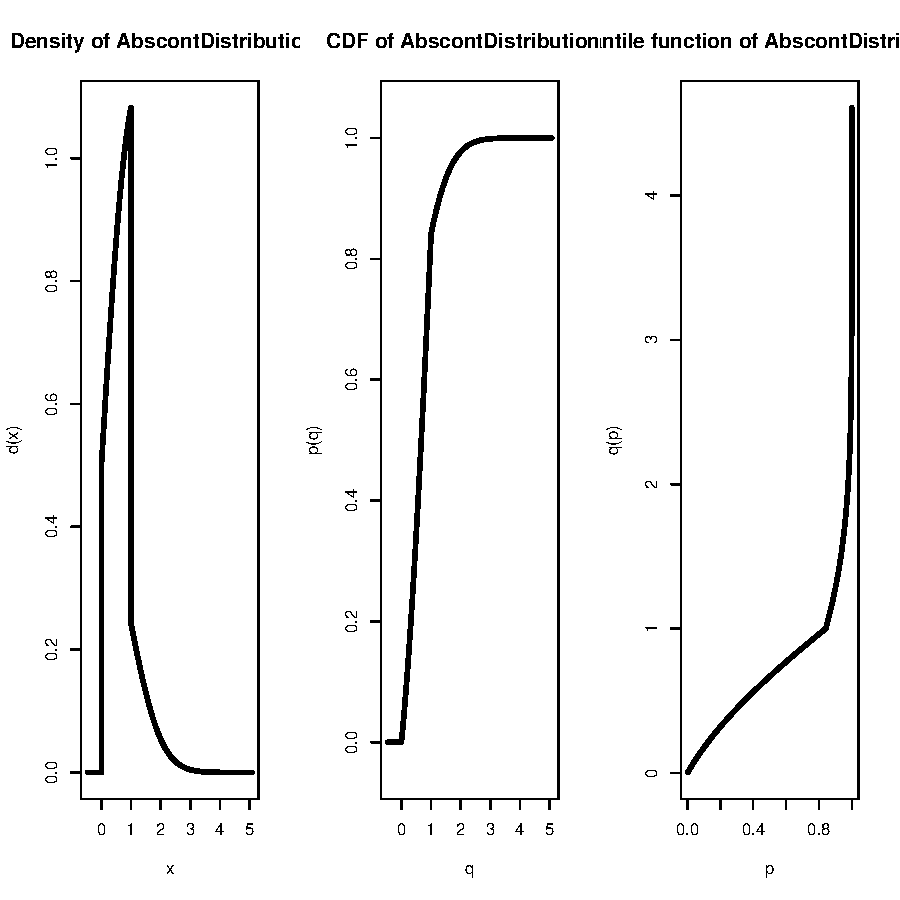
\includegraphics{distr-minandmax}
\begin{Schunk}
\begin{Sinput}
> Z <- Minimum(N, U)
> plot(Z)
\end{Sinput}
\end{Schunk}
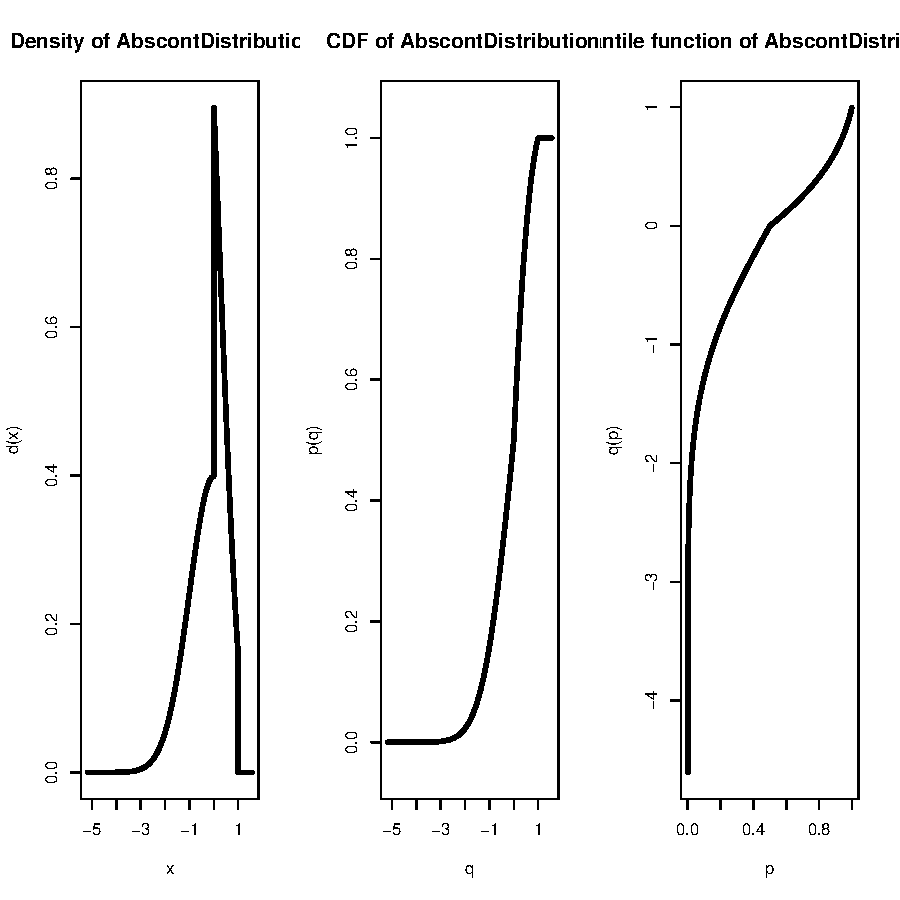
\includegraphics{distr-min}
\subsection{Instructive destructive example}\label{destrex}
\begin{footnotesize}
  Code also available under\newline \href{http://www.uni-bayreuth.de/departments/math/org/mathe7/DISTR/destructive.R}%
  {\parbox[t]{12cm}{$\mbox{\hspace{2cm}}${\tt http://www.uni-bayreuth.de/departments/math/org/}\\%
  {$\mbox{\hspace{2cm}}$\hphantom{\tt http:/}{\tt /mathe7/DISTR/destructive.R}}}}\\[2ex]
\end{footnotesize}
\begin{Schunk}
\begin{Sinput}
> require(distr)
\end{Sinput}
\begin{Soutput}
[1] TRUE
\end{Soutput}
\begin{Sinput}
> N <- Norm()
> B <- Binom()
> N@d <- B@d
> plot(N)
\end{Sinput}
\end{Schunk}
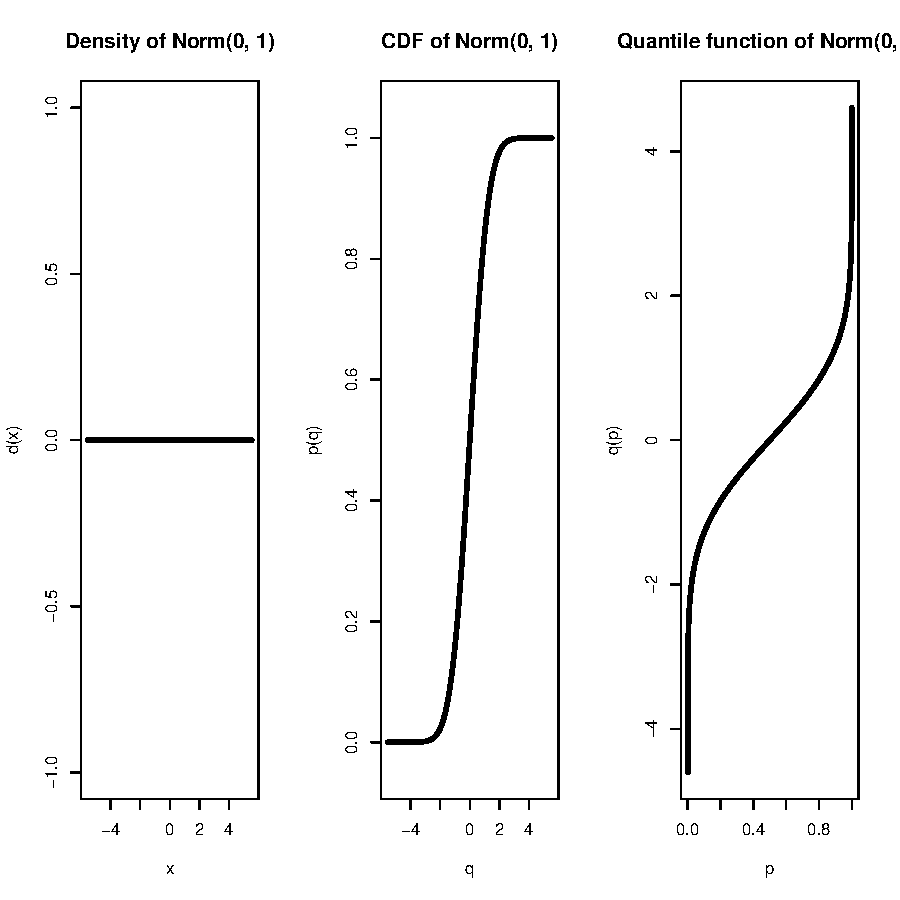
\includegraphics{distr-destructive}
\subsection{A simulation example}\label{simex}
{\bf needs packages \pkg{distrSim}/\pkg{distrTEst}}\\[2ex]
\begin{footnotesize}
  Code also available under\newline \href{http://www.uni-bayreuth.de/departments/math/org/mathe7/DISTR/SimulateandEstimate.R}%
  {\parbox[t]{12cm}{$\mbox{\hspace{2cm}}${\tt http://www.uni-bayreuth.de/departments/math/org/}\\%
  {$\mbox{\hspace{2cm}}$\hphantom{\tt http:/}{\tt /mathe7/DISTR/SimulateandEstimate.R}}}}\\[2ex]
\end{footnotesize}
\begin{Schunk}
\begin{Sinput}
> have.distrTEst <- suppressWarnings(require(distrTEst))
> if (have.distrTEst) {
+     sim <- new("Simulation", seed = setRNG(), distribution = Norm(mean = 0, 
+         sd = 1), filename = "sim_01", runs = 1000, samplesize = 30)
+     contsim <- new("Contsimulation", seed = setRNG(), distribution.id = Norm(mean = 0, 
+         sd = 1), distribution.c = Norm(mean = 0, sd = 9), rate = 0.1, 
+         filename = "contsim_01", runs = 1000, samplesize = 30)
+     simulate(sim)
+     simulate(contsim)
+     print(sim)
+     summary(contsim)
+     plot(contsim)
+ } else {
+     cat("\n functionality not (yet) available; ")
+     cat("you have to install package \"distrTEst\" first.\n")
+ }
\end{Sinput}
\begin{Soutput}
filename of Simulation: sim_01
seed of Simulation: Mersenne-Twister
 seed of Simulation: Inversion
 seed of Simulation: c(312, 992586505, -1091336977, -1873268990, 1830591758, 568584456, -1733810521, -193247257, 407903804, 853277018, -1291849909, 690983857, -1222907145, 1349331796, -1956014272, 2049648770, 1722259598, 18384930, -1660853598, -1504143456, 676636782, -1307850353, 885336488, 493255236, 2101148134, 1065335730, -912707068, -1967312219, -702172411, -108588300, -233389314, 396170801, -270615063, 1488113139, -650897964, -885276147, 2107126223, -1747657349, -398195964, -1216170335, -1670286632, -1409033516, 
number of runs: 1000
dimension of the observations: 1
size of sample: 30
object was generated by version: 1.8
Distribution:
Distribution Object of Class: Norm
mean :  0 
sd :  1 
name of simulation: contsim_01
rate of contamination: 0.100000
real Data:
dimension of the observations: 1
number of runs: 1000
size of sample: 30
\end{Soutput}
\end{Schunk}
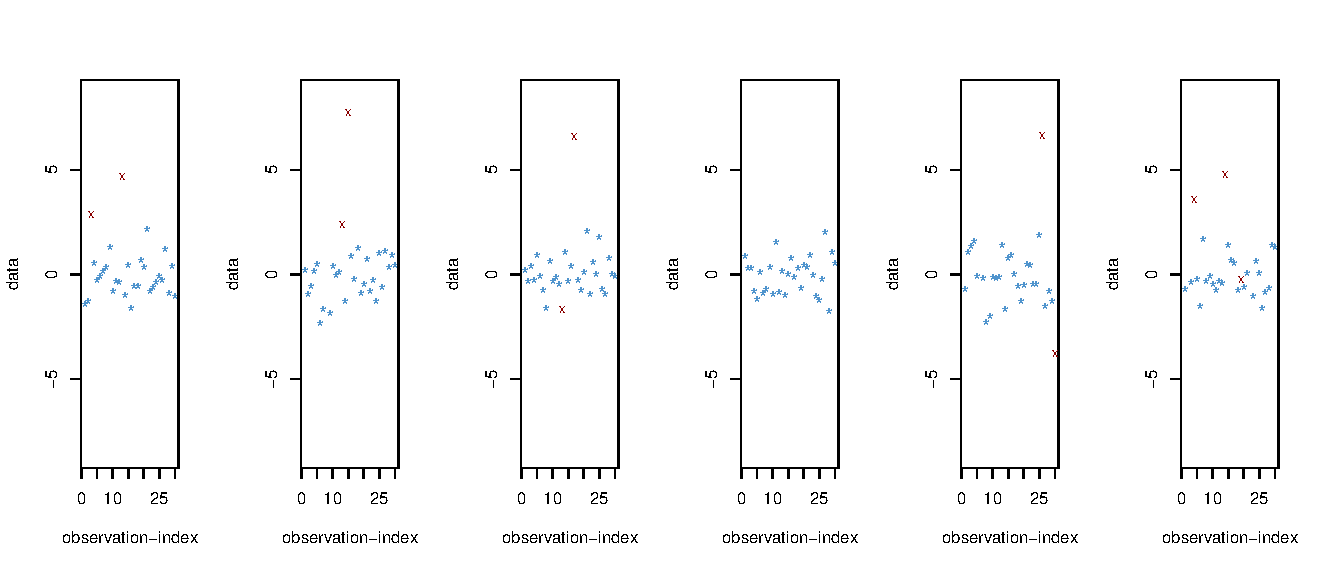
\includegraphics{distr-SimulateandEstimate}
\begin{Schunk}
\begin{Sinput}
> have.distrTEst <- suppressWarnings(require("distrTEst"))
> if (have.distrTEst) {
+     psim <- function(theta, y, m0) {
+         mean(pmin(pmax(-m0, y - theta), m0))
+     }
+     mestimator <- function(x, m = 0.7) {
+         uniroot(psim, low = -20, up = 20, tol = 1e-10, y = x, 
+             m0 = m, maxiter = 20)$root
+     }
+     result.id.mean <- evaluate(sim, mean)
+     result.id.mest <- evaluate(sim, mestimator)
+     result.id.median <- evaluate(sim, median)
+     result.cont.mean <- evaluate(contsim, mean)
+     result.cont.mest <- evaluate(contsim, mestimator)
+     result.cont.median <- evaluate(contsim, median)
+     elist <- EvaluationList(result.cont.mean, result.cont.mest, 
+         result.cont.median)
+     print(elist)
+     summary(elist)
+     plot(elist, cex = 0.7)
+ } else {
+     cat("\n functionality not (yet) available; ")
+     cat("you have to install package \"distrTEst\" first.\n")
+ }
\end{Sinput}
\begin{Soutput}
An EvaluationList Object
name of Evaluation List: a list of "Evaluation" objects
name of Dataobject: object
name of Datafile: contsim_01
----------------------------------
An Evaluation Object
estimator: mean
Result: 'data.frame':	1000 obs. of  2 variables:
 $ mean.id: num  -0.13697  0.06051  0.00985 -0.04599  0.43008 ...
 $ mean.re: num  -0.064  0.991 -0.445  0.237  1.423 ...
----------------------------------
An Evaluation Object
estimator: mestimator
Result: 'data.frame':	1000 obs. of  2 variables:
 $ mstm.id: num  -0.0720  0.0621  0.0818 -0.0753  0.3795 ...
 $ mstm.re: num  -0.0483  0.5620  0.0514  0.1390  0.5566 ...
----------------------------------
An Evaluation Object
estimator: median
Result: 'data.frame':	1000 obs. of  2 variables:
 $ medn.id: num  0.10299 0.00262 0.15605 0.05464 0.30376 ...
 $ medn.re: num  0.103 0.681 0.156 0.260 0.465 ...
name of Evaluation List: a list of "Evaluation" objects
name of Dataobject: object
name of Datafile: contsim_01
----------------------------------
name of Evaluation: object
estimator: mean
Result:
    mean.id             mean.re        
 Min.   :-0.647788   Min.   :-1.95427  
 1st Qu.:-0.116459   1st Qu.:-0.34752  
 Median : 0.004664   Median :-0.01436  
 Mean   : 0.005352   Mean   :-0.01149  
 3rd Qu.: 0.126965   3rd Qu.: 0.29756  
 Max.   : 0.567246   Max.   : 1.80795  
----------------------------------
name of Evaluation: object
estimator: mestimator
Result:
    mstm.id             mstm.re         
 Min.   :-0.680226   Min.   :-0.685379  
 1st Qu.:-0.123801   1st Qu.:-0.148639  
 Median :-0.004340   Median :-0.002694  
 Mean   : 0.004876   Mean   : 0.002649  
 3rd Qu.: 0.136163   3rd Qu.: 0.148642  
 Max.   : 0.663399   Max.   : 0.663399  
----------------------------------
name of Evaluation: object
estimator: median
Result:
    medn.id             medn.re         
 Min.   :-0.711295   Min.   :-0.757078  
 1st Qu.:-0.136414   1st Qu.:-0.150264  
 Median : 0.000839   Median :-0.001653  
 Mean   : 0.008166   Mean   : 0.005374  
 3rd Qu.: 0.150733   3rd Qu.: 0.167842  
 Max.   : 0.706914   Max.   : 0.706914  
\end{Soutput}
\end{Schunk}
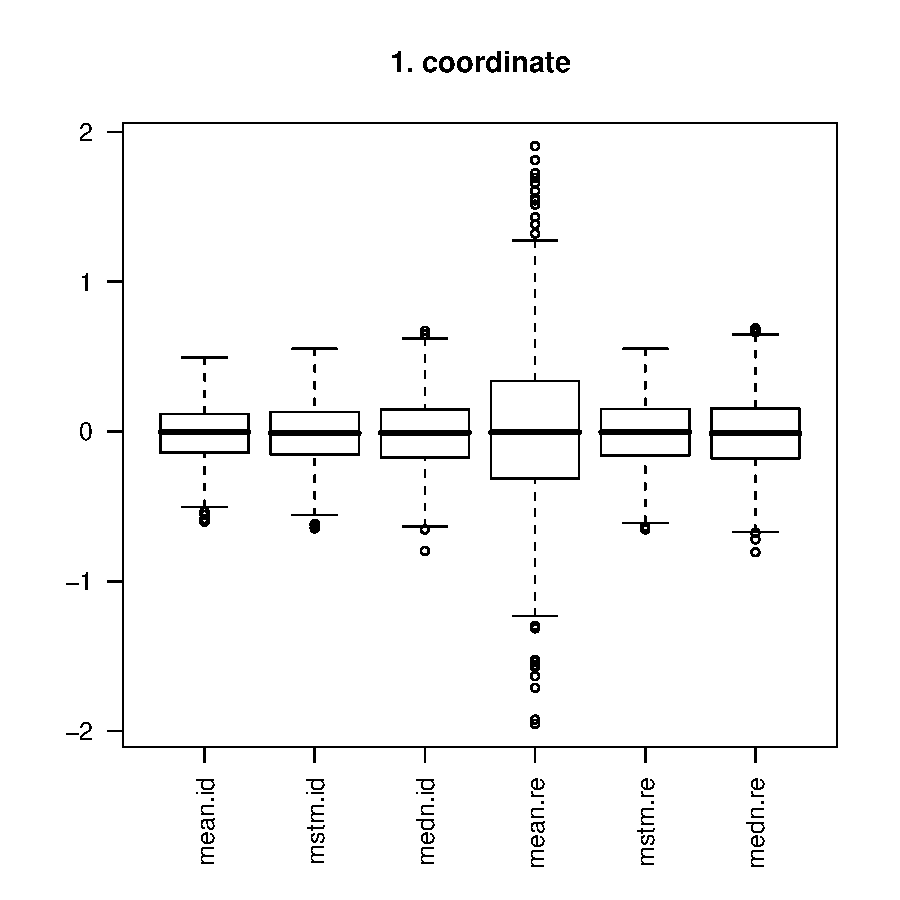
\includegraphics{distr-elist}
\par
\begin{footnotesize}
Output by \code{plot}/\code{show}-method for an object of class \code{Evaluation}
\begin{Schunk}
\begin{Sinput}
> result.cont.mest
\end{Sinput}
\begin{Soutput}
An Evaluation Object
name of Dataobject: object
name of Datafile: contsim_01
estimator: mestimator
Result: 'data.frame':	1000 obs. of  2 variables:
 $ mstm.id: num  -0.0720  0.0621  0.0818 -0.0753  0.3795 ...
 $ mstm.re: num  -0.0483  0.5620  0.0514  0.1390  0.5566 ...
\end{Soutput}
\end{Schunk}
\end{footnotesize}
\begin{footnotesize}
Output by \code{summary}-method for an object of class \code{EvaluationList}
\begin{Schunk}
\begin{Sinput}
> summary(elist)
\end{Sinput}
\begin{Soutput}
name of Evaluation List: a list of "Evaluation" objects
name of Dataobject: object
name of Datafile: contsim_01
----------------------------------
name of Evaluation: object
estimator: mean
Result:
    mean.id             mean.re        
 Min.   :-0.647788   Min.   :-1.95427  
 1st Qu.:-0.116459   1st Qu.:-0.34752  
 Median : 0.004664   Median :-0.01436  
 Mean   : 0.005352   Mean   :-0.01149  
 3rd Qu.: 0.126965   3rd Qu.: 0.29756  
 Max.   : 0.567246   Max.   : 1.80795  
----------------------------------
name of Evaluation: object
estimator: mestimator
Result:
    mstm.id             mstm.re         
 Min.   :-0.680226   Min.   :-0.685379  
 1st Qu.:-0.123801   1st Qu.:-0.148639  
 Median :-0.004340   Median :-0.002694  
 Mean   : 0.004876   Mean   : 0.002649  
 3rd Qu.: 0.136163   3rd Qu.: 0.148642  
 Max.   : 0.663399   Max.   : 0.663399  
----------------------------------
name of Evaluation: object
estimator: median
Result:
    medn.id             medn.re         
 Min.   :-0.711295   Min.   :-0.757078  
 1st Qu.:-0.136414   1st Qu.:-0.150264  
 Median : 0.000839   Median :-0.001653  
 Mean   : 0.008166   Mean   : 0.005374  
 3rd Qu.: 0.150733   3rd Qu.: 0.167842  
 Max.   : 0.706914   Max.   : 0.706914  
\end{Soutput}
\end{Schunk}
\end{footnotesize}
\begin{small}
In this example we present a standard robust simulation study that --- in variations --- arises in almost
every paper on Robust Statistics. We do this with the tools provided by our package\ldots
\end{small}
\subsection{Expectation of a given function under a given distribution}
\begin{footnotesize}
  Code also available under\newline \href{http://www.uni-bayreuth.de/departments/math/org/mathe7/DISTR/Expectation.R}%
  {\parbox[t]{12cm}{$\mbox{\hspace{2cm}}${\tt http://www.uni-bayreuth.de/departments/math/org/}\\%
  {$\mbox{\hspace{2cm}}$\hphantom{\tt http:/}{\tt /mathe7/DISTR/Expectation.R}}}}\\[2ex]
  This code is for illustration only; in the mean-time, the expectation- and variance operators implemented
  in this example have been included to package \pkg{distrEx} where their functionality has further been extended.
\end{footnotesize}
\begin{small}
As in examples~\ref{truncex} and \ref{minmaxex}, we illustrate the use of package {\tt "distr"} by implementing
a general evaluation of expectation and variance under a given distribution.
\end{small}
\begin{Schunk}
\begin{Sinput}
> have.distrEx <- suppressWarnings(require("distrEx"))
> if (have.distrEx) {
+     id <- function(x) x
+     sq <- function(x) x^2
+     B <- Binom(6, 0.5)
+     E(B, id)
+     E(B, sq) - E(B, id)^2
+     N <- Norm(1, 1)
+     E(N, id)
+     E(N, sq) - E(N, id)^2
+ } else {
+     cat("\n functionality not (yet) available; ")
+     cat("you have to install package \"distrEx\" first.\n")
+ }
\end{Sinput}
\begin{Soutput}
[1] 1
\end{Soutput}
\end{Schunk}
\subsection{$n$-fold convolution of absolutely continuous distributions}\label{exe10}
\begin{footnotesize}
  Code also available under\newline \href{http://www.uni-bayreuth.de/departments/math/org/mathe7/DISTR/nFoldConvolution.R}%
  {\parbox[t]{12cm}{$\mbox{\hspace{2cm}}${\tt http://www.uni-bayreuth.de/departments/math/org/}\\%
  {$\mbox{\hspace{2cm}}$\hphantom{\tt http:/}{\tt /mathe7/DISTR/nFoldConvolution.R}}}}\\[2ex]
\end{footnotesize}
\begin{small}
Might be useful for teaching the CLT: a straightforward implementation of the $n$--fold convolution of an
arbitrary implemented absolutely continuous distribution --- to show accuracy of our method we compare it to the
exact formula valid for $n$-fold convolution of normal distributions.
\end{small}
\begin{Schunk}
\begin{Sinput}
> require(distr)
\end{Sinput}
\begin{Soutput}
[1] TRUE
\end{Soutput}
\begin{Sinput}
> if (!isGeneric("convpow")) setGeneric("convpow", function(D1, 
+     N) standardGeneric("convpow"))
\end{Sinput}
\begin{Soutput}
[1] "convpow"
\end{Soutput}
\begin{Sinput}
> setMethod("convpow", signature(D1 = "AbscontDistribution", N = "numeric"), 
+     function(D1, N) {
+         if ((N < 1) || (!identical(floor(N), N))) 
+             stop("N has to be a natural greater than 0")
+         m <- getdistrOption("DefaultNrFFTGridPointsExponent")
+         lower <- ifelse((q(D1)(0) > -Inf), q(D1)(0), q(D1)(getdistrOption("TruncQuantile")))
+         upper <- ifelse((q(D1)(1) < Inf), q(D1)(1), q(D1)(1 - 
+             getdistrOption("TruncQuantile")))
+         M <- 2^m
+         h <- (upper - lower)/M
+         if (h > 0.01) 
+             warning(paste("Grid for approxfun too wide, ", "increase DefaultNrFFTGridPointsExponent", 
+                 sep = ""))
+         x <- seq(from = lower, to = upper, by = h)
+         p1 <- p(D1)(x)
+         p1 <- p1[2:(M + 1)] - p1[1:M]
+         pn <- c(p1, numeric((N - 1) * M))
+         fftpn <- fft(pn)
+         pn <- Re(fft(fftpn^N, inverse = TRUE))/(N * M)
+         pn <- (abs(pn) >= .Machine$double.eps) * pn
+         i.max <- N * M - (N - 2)
+         pn <- c(0, pn[1:i.max])
+         dn <- pn/h
+         pn <- cumsum(pn)
+         x <- c(N * lower, seq(from = N * lower + N/2 * h, to = N * 
+             upper - N/2 * h, by = h), N * upper)
+         dnfun1 <- approxfun(x = x, y = dn, yleft = 0, yright = 0)
+         standardizer <- sum(dn[2:i.max]) + (dn[1] + dn[i.max + 
+             1])/2
+         dnfun2 <- function(x) dnfun1(x)/standardizer
+         pnfun1 <- approxfun(x = x + 0.5 * h, y = pn, yleft = 0, 
+             yright = pn[i.max + 1])
+         pnfun2 <- function(x) pnfun1(x)/pn[i.max + 1]
+         yleft <- ifelse(((q(D1)(0) == -Inf) | (q(D1)(0) == -Inf)), 
+             -Inf, N * lower)
+         yright <- ifelse(((q(D1)(1) == Inf) | (q(D1)(1) == Inf)), 
+             Inf, N * upper)
+         w0 <- options("warn")
+         options(warn = -1)
+         qnfun1 <- approxfun(x = pnfun2(x + 0.5 * h), y = x + 
+             0.5 * h, yleft = yleft, yright = yright)
+         qnfun2 <- function(x) {
+             ind1 <- (x == 0) * (1:length(x))
+             ind2 <- (x == 1) * (1:length(x))
+             y <- qnfun1(x)
+             y <- replace(y, ind1[ind1 != 0], yleft)
+             y <- replace(y, ind2[ind2 != 0], yright)
+             return(y)
+         }
+         options(w0)
+         rnew = function(N) apply(matrix(r(e1)(n * N), ncol = N), 
+             1, sum)
+         return(new("AbscontDistribution", r = rnew, d = dnfun1, 
+             p = pnfun2, q = qnfun2))
+     })
\end{Sinput}
\begin{Soutput}
[1] "convpow"
\end{Soutput}
\begin{Sinput}
> A <- Norm(mean = 0, sd = 1)
> N <- 10
> AN <- convpow(A, N)
> AN1 <- Norm(mean = 0, sd = sqrt(N))
> eps <- getdistrOption("TruncQuantile")
> par(mfrow = c(1, 3))
> low <- q(AN1)(eps)
> upp <- q(AN1)(1 - eps)
> x <- seq(from = low, to = upp, length = 10000)
> plot(x, d(AN1)(x), type = "l", lwd = 5)
> lines(x, d(AN)(x), col = "orange", lwd = 1)
> title("Densities")
> legend(low, d(AN)(0), legend = c("exact", "FFT"), fill = c("black", 
+     "orange"))
> plot(x, p(AN1)(x), type = "l", lwd = 5)
> lines(x, p(AN)(x), col = "orange", lwd = 1)
> title("Cumulative distribution functions")
> legend(low, 1, legend = c("exact", "FFT"), fill = c("black", 
+     "orange"))
> x <- seq(from = eps, to = 1 - eps, length = 1000)
> plot(x, q(AN1)(x), type = "l", lwd = 5)
> lines(x, q(AN)(x), col = "orange", lwd = 1)
> title("Quantile functions")
> legend(0, q(AN1)(1 - eps), legend = c("exact", "FFT"), fill = c("black", 
+     "orange"))
\end{Sinput}
\end{Schunk}
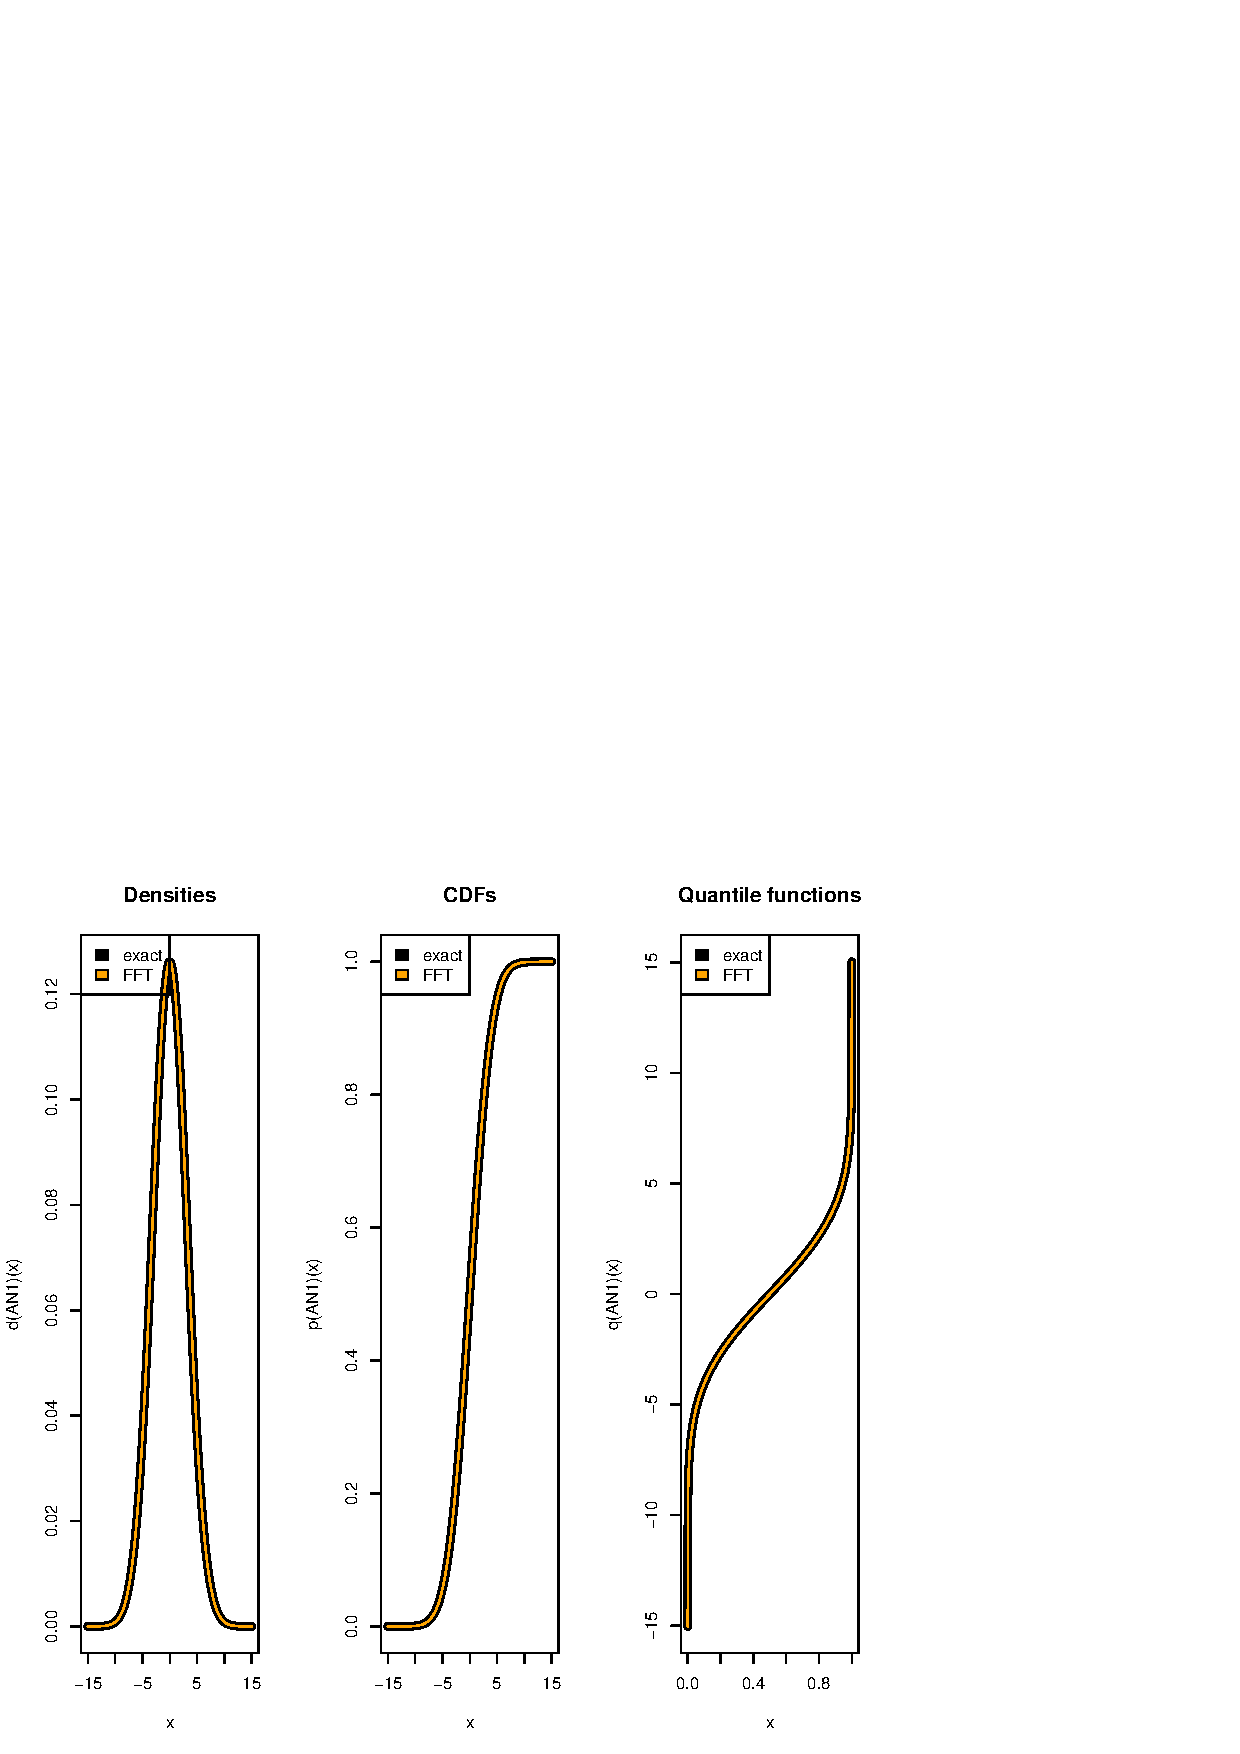
\includegraphics{distr-nFoldConvolution}
%-------------------------------------------------------------------------------
\begin{thebibliography}{8}

\bibitem{Beng:03}
Bengtsson H. 
\newblock The {R.oo} package - object-oriented programming with references using standard {R} code.
\newblock In: Hornik K., Leisch F. and Zeileis A. (Eds.) {\em
  Proceedings of the 3rd International Workshop on Distributed Statistical
  Computing (DSC 2003)\/}. Vienna, Austria.
\newblock Published as http://www.ci.tuwien.ac.at/Conferences/DSC-2003/ 

\bibitem{Cham:98}
Chambers J.M. 
\newblock {\em {Programming with data. A guide to the S language}\/}.
\newblock {Springer}.
\newblock http://cm.bell-labs.com/stat/Sbook/index.html

\bibitem{OOPGent}
Gentleman R.
\newblock {\em Object Orientated Programming. Slides of a Short Course held in Auckland\/}.
\newblock http://www.stat.auckland.ac.nz/S-Workshop/Gentleman/Methods.pdf

\bibitem{MK:05}
Kohl M. 
\newblock {\em Numerical Contributions to the Asymptotic Theory of Robustness\/}. 
\newblock {Dissertation}, Universit\"at Bayreuth. 
\newblock See also http://stamats.de/ThesisMKohl.pdf

\bibitem{K:R:S:04}
Kohl M., Ruckdeschel P. and Stabla T.
\newblock {General Purpose Convolution Algorithm for Distributions in S4-Classes by means of FFT}.
\newblock unpublished manual

\bibitem{NumR:92}
Press W.H., Teukolsky S.A., Vetterling W.T. and Flannery B.P.
\newblock {\em {Numerical recipes in C. The art of scientific computing.}\/}
\newblock {Cambridge Univ. Press}, 2. Aufl.

\bibitem{Ric:88}
Rice J.A. 
\newblock {\em {Mathematical statistics and data analysis}\/}.
\newblock The Wadsworth \& Brooks/Cole Statistics/Probability Series.
  {Wadsworth \& Brooks/Cole Advanced Books \& Software}, Pacific Grove,
  California.

\bibitem{R:K:S:C:04}
Ruckdeschel P., Kohl M., Stabla T., and Camphausen F. 
\newblock {S4 Classes for Distributions.} 
\newblock {\em R-News\/}, {\bf 6}(2): 10--13.
\newblock http://CRAN.R-project.org/doc/Rnews/Rnews\_2006-2.pdf
%\newblock See also {http://www.uni-bayreuth.de/departments/math/org/mathe7/RUCKDESCHEL/pubs/distr.pdf}

\end{thebibliography}
% -------------------------------------------------------------------------------
\end{document}
% -------------------------------------------------------------------------------
